\section{From micro-physics to thermodynamics: Equazione di stato per ioni ed elettroni}

%\begin{multicols}{2}%https://newbedev.com/how-to-explicitly-split-long-toc-in-beamer
%   \tableofcontents[currentsection]{cherryframes}
%\end{multicols}

\begin{wordonframe}{Schema fisico/chimico: relazione $\rho(P,T)$ realistiche}
\begin{itemize}
\item schema  chimico: il primo considera atomi e molecole, la cui popolazione per stati eccitati e diversi gradi di ionizzazione \'e ottenuto minimizzando l'energia libera da cui sono ricavate le altre grandezze termodinamiche; utilizzando questo approccio \'e stata ricavata l'equazione di stato MHD (\cite{hummer1988equation})
\item schema fisico: nuclei ed elettroni come costituenti fondamentali interagenti tramite potenziale Coulombiano e trova le soluzione dell'equazione di Schr\"oedinger per un problema a molti corpi, questo approccio, usato per ricavare l'equazione di stato OPAL (\cite{rogers1986occupation})
\end{itemize}
Come illustrato in figura, per entrambe $\Gamma_1\approx\midfrac{5}{3}$ nell'interno solare e maggiori deviazioni si hanno nelle regioni di ionizzazione parziale degli elementi in particolare di idrogeno ed elio.
\end{wordonframe}

\begin{wordonframe}{Relazione tra $P(\rho, T)$: approx zero gas perfetto di atomi completamente ionizzati}
\begin{columns}[T]%
% \hspace{-19pt}\relax
\begin{column}{0.55\textwidth}%
EOS gas perfetto di ioni ed elettroni 
\begin{align*}
    &P_G=P_I+P_e=\frac{\rho}{\mu}\gasconstant{}T=nKT=\frac{\rho}{\mu m_u}KT\tag{$R=N_AK$}\\
&\frac{d\rho}{\rho}=\frac{dP}{P}-\frac{dT}{T}+\frac{d\mu}{\mu}\\
&(\frac{d\rho}{\rho}=\alpha\frac{dP}{P}-\delta\frac{dT}{T}+\phi\frac{d\mu}{\mu})
\end{align*}
Energia interna per unit\'a di massa: somma delle energie traslazionali delle particelle pesate secondo la distribuzione di equilibrio di Maxwell-Boltzmann per grammo di materia
 \begin{align*}
&u=\frac{1}{\rho}\sum_i\int f^{(0)}(\vec{p}_i)\frac{p^2_i}{2m_i}\,d^3p_i\\
&=\frac{3}{2}\frac{P}{\rho}=\frac{3}{2}\frac{\gasconstant T}{\mu}
\end{align*}
\end{column}
 %   \hspace{-22pt}\relax
\begin{column}{0.45\textwidth}
Peso molecolare medio: massa media in amu per particella libera
\begin{align*}
&\mu=\frac{1}{\bar{n}_HX+\bar{n}_{He}Y+\bar{n}_{Z}Z}\\
&\invers{\mu}=\sum_i X_i \frac{1+f_i}{A_i}\\
&\mu_0=\frac{1}{X+\midfrac{Y}{4}+\midfrac{Z}{\bar{A}}},\ \mu_e\approx\frac{2}{1+X}
\end{align*}
con $\bar{n}_i=\frac{1+f_i}{A_i}$ numero medio di particelle libere per unit\'a di massa atomica dovute alla specie i di peso atomico $A_i$ e $f_i$ numero medio di elettroni liberati da ione della specie i; peso atomico medio per ione $\mu_0$ ed elettrone libero (ionizzato) $\mu_e$.
\end{column}
\end{columns}
$f^{(0)}(\vec{p}_i)$: numero di particelle della specie i per unit\'a di volume con impulso in $[\vec{p}_i,\vec{p}_i+d\vec{p}_i]$
\end{wordonframe}

\begin{wordonframe}{Deviazioni dalla legge dei gas perfetti: radiazione e degenerazione elettronica}
\begin{itemize}
	\item Radiazione. Il contributo alla pressione ed energia interna per unit\'a di volume dei fotoni $P_R=\frac{a}{3}T^4$, $u_R=aT^4$, e $P-P_R=\beta P$.
	\item Degenerazione elettronica - Principio di Pauli: non pi\'u di 2 elettroni in volume di spazio delle fasi $h^3$. $n_e$ la densit\'a numerica di \Pelectron, $\psi(P,T)$ il parametro di degenerazione, tale che per $\psi\to-\infty$ si abbia la distribuzione di Boltzmann e per $\psi\to+\infty$ completa degenerazione
	\begin{align*}
	&n_e=\rho N_A\frac{1+X}{2}=\intzi{}\frac{8\pi p^2\,dp}{h^3(\exp{\frac{u_k}{KT}-\psi}+1)}=\frac{8\pi}{h^3}(2m_ekT)\expy{3/2}a(\psi)\\
	&P_e=\beta P-\rho\gasconstant{}(X+\frac{Y}{4}+\frac{Z}{\exv{A_Z}})=\frac{8\pi}{3h^3}\intzi{}p^3v(p)\frac{dp}{1+\exp{\epsilon/kT-\psi}}\\
	&U_e=\frac{8\pi}{h^3}\int_0^{\infty}\frac{p^2\epsilon(p)\,dp}{\exp{(-\psi+\midfrac{\epsilon}{KT})}+1}
	\end{align*}
\end{itemize}
\end{wordonframe}

\begin{frame}{degenerazione completa: casi limite NR e R}
    Quantum cell of volume in P.S. $d^3pd^3x=h^3$ each with $g_e=2$: in shell $[p,p+dp]$ there are $\frac{4\pi p^2dpdV}{h^3}$ so $f(p)dpdV\leq \frac{2*4\pi p^2\,dpdV}{h^3}$. Complete degeneracy: $f(p)=\left\{\begin{array}{l}
            \frac{4\pi p^2}{h^3}:\ p\leq p_F\\
            0\\
    \end{array}\right.$, so $n_edV=dV\int_0^{p_F}\frac{8\pi p^2}{h^3},dp=\frac{8\pi}{3h^3}p_F^3dV$. Given $n_e$ we get $p_F\propto n_e^{\frac{1}{3}}$
    \begin{columns}[T]
        \begin{column}{0.4\textwidth}
            NR: $E_F=\frac{p_F^2}{2m_e}\propto n_e^{\frac{2}{3}}$        
        \end{column}
        \begin{column}{0.6\textwidth}
            R: If $n_e$ such that $p_F$ relativistic
            \begin{align*}
                &p=\frac{m_ev}{\sqrt{1-(\frac{v}{c})^2}},E_T=\frac{m_ec^2}{\sqrt{1-(\frac{v}{c})^2}}=m_ec^2\sqrt{1+\frac{p^2}{m_e^2c^2}}\\
                &\Rightarrow \frac{1}{c}\TDy{p}{E_T}=\frac{\frac{p}{m_ec}}{\sqrt{1+\frac{p^2}{m_e^2c^2}}}\\
                &E=E_T-m_ec^2\\
            \end{align*}
        \end{column}
    \end{columns}
    For EOS we need pressure (flux of momentum per unit surf per second: surf $d\sigma$, normal $\vec{n}$).Let's determine number of electrons goin through $d\sigma$ into small solid angle $d\Omega_s$ around dir $\vec{s}$ with $[p,p+dp]$: $f(p)\,dp \frac{d\Omega_s}{4\pi}$ electrons per unit volume with right p and dir, having $f(p)\,dpv(p)\cos{\theta}\,d\sigma \frac{d\Omega_s}{4\pi}$ electrons going through the surface per sec into $d\Omega_s$; total flux of momentum in dir $\vec{n}$ is
    \begin{align*}
        &P_e=\int_{2\pi}\frac{d\Omega_s}{4\pi}\int_0^{\infty}f(p)v(p)p\cos^2{\theta}\,dp=\frac{8\pi}{3h^3}\int_0^{p_F}p^3v(p)\,dp\tag{$\frac{4\pi}{3}$ int of $\cos^2{\theta}$ over hemisphere}\\
        &
    \end{align*}
\end{frame}

\begin{frame}{EOS complete degenerate electron gas}
\begin{align*}
    &P_e=\frac{8\pi c}{3h^3}\int_0^{P_F}\frac{p/(m_ec)}{\sqrt{1+p^2/(m_ec)^2}}=\frac{8\pi c^5 m_e^4}{3h^3}\int_0^x \frac{\xi^4\,d\xi}{\sqrt{1+\xi^2}}\tag{$\xi=\frac{p}{m_ec}$, $x=\frac{p_F}{m_ec}$: $n_e=\frac{\rho}{\mu_em_u}=\frac{8\pi m_e^3c^3}{3h^3}x^3$}\\
    &P_e=\frac{\pi m_e^4c^5}{3h^2}f(x),\ \int_0^x \frac{\xi^4\,d\xi}{\sqrt{1+\xi^2}}=\frac{1}{8}[x(2x^2-3)\sqrt{1+x^2}+3\sinh^{-1}{x}]\\
    &U_e=\int_0^{P_F}f(p)E(p)\,dp=\frac{8\pi}{h^3}\int_0^{P_F}E(p)p^2\,dp=\frac{\pi m_e^4c^5}{3h^3}g(x),\ g(x)=8x^3[\sqrt{x^2+1}-1]-f(x)\\
\end{align*}
x measures importance of rel. effect for electrons with high mom., $x=\frac{p_F}{m_ec}=\frac{\frac{v_F}{c}}{\sqrt{1-(\frac{v_f}{c})^2}}$ or $\frac{v_F^2}{c^2}=\frac{x^2}{1+x^2}$: if $x\ll1$ then $\frac{v_F}{c}\ll1$ (NR), if $x\gg1$ then $\frac{v_F}{c}\approx1$
\begin{align*}
    &x\to0: f(x)\to \frac{8}{5}x^5,\ g(x)\to \frac{12}{5}x^5\\
    &x\to\infty:\ f(x)\to 2x^4,\ g(x)\to6x^4\\
    &\Rightarrow P_e=\frac{8\pi m_e^4c^5}{15h^3}x^5=\frac{2}{3}U_e\tag{$x\ll1$}\\
    &P_e=\frac{1}{20}(\frac{3}{\pi})^{\frac{2}{3}}\frac{h^2}{m_e}n_e^{\frac{5}{3}}=\frac{1}{20}(\frac{3}{\pi})^{\frac{2}{3}}\frac{h^2}{m_em_u^{\frac{5}{3}}}(\frac{\rho}{\mu_e})^{\frac{5}{3}}=\num{1.0036e13}(\frac{\rho}{\mu_e})\expy{5/3}\si{\cgs}\tag{EOS comp-deg-NR-\Pelectron}\\
    &\Rightarrow P_e=\frac{2\pi m_e^4c^5}{3h^3}x^4=\frac{1}{3}U_e\tag{$x\gg1$}\\
    &=(\frac{3}{\pi})^{\frac{1}{3}}\frac{hc}{8}n_e^{\frac{4}{3}}=(\frac{3}{\pi})^{\frac{1}{3}}\frac{hc}{8m_u^{\frac{4}{3}}}(\frac{\rho}{\mu_e})^{\frac{4}{2}}=\num{1.2435e15}(\frac{\rho}{\mu_e})\expy{4/3}\si{\cgs}\tag{EOS comp-deg-UR-\Pelectron}
\end{align*}
\end{frame}

\begin{frame}{Partial degeneracy of electron gas}
    \begin{columns}[T]
        \begin{column}{0.65\textwidth}
    For finite T not all \Pelectron will be in cell of lowest poss. moment: most prob. occupation of phase cells of shell $[p,p+dp]$ is determined by $f(p)\,dp\,dV=\frac{8\pi p^2\,dpdV}{h^3}\frac{1}{1+\exp{\frac{E}{KT}-\psi}}$, $\psi$ deg. param.
        \end{column}
        \begin{column}{0.35\textwidth}
            \begin{align*}
                &n_e=\frac{8\pi}{h^3}\int_0^{\infty}\frac{p^2\,dp}{1+\exp{\frac{E}{KT}-\psi}}\\
                &P_e=\frac{8\pi}{3h^3}\int_0^{\infty}p^3v(p)\frac{p^2\,dp}{1+\exp{\frac{E}{KT}-\psi}}\\
                &U_e=\frac{8\pi}{h^3}\int_0^{\infty}\frac{Ep^2\,dp}{1+\exp{\frac{E}{KT}-\psi}}\\
            \end{align*}
        \end{column}
    \end{columns}
    \begin{columns}[T]
        \begin{column}{0.55\textwidth}
            NR: $E=\frac{p^2}{2m}$
            \begin{align*}
                &n_e=\frac{8\pi}{h^3}\int_0^{\infty}\frac{p^2\,dp}{1+\exp{\frac{E}{KT}-\psi}}=\frac{8\pi}{h^3}(2m_eKT)^{\frac{3}{2}}a(\psi)\\
                &a(\psi)=\int_0^{\infty}\frac{\eta^2\,d\eta}{1+\exp{\eta^2-\psi}},\ \eta=\frac{p}{\sqrt{2m_eKT}}\\
                &\Rightarrow \psi=\psi(\frac{n_e}{T^{\frac{3}{2}}})\\
                &\exp{\psi}=\frac{h^3n_e}{2(2\pi m_eKT)^{\frac{3}{2}}}\tag{$\psi\to-\infty$, large T, $f(p)$ becomes Boltzman}\\
                &\psi=\frac{E_0}{KT}\tag{$\psi\to\infty$}\\
                &\frac{1}{1+\exp{\frac{E}{KT}-\psi}}=\frac{1}{1+\exp{\psi(\frac{E}{E_0}-1)}}\approx\left\{\begin{array}{l}
                        1:\ E<E_0\\
                        0:\ E>E_0\\
                    \end{array}\\
            \end{align*}
        \end{column}
        \begin{column}{0.45\textwidth}
            \begin{align*}
                    &n_e=\frac{\rho}{\mu_em_u}\\
                    &=\frac{4\pi}{h^3}(2m_eKT)^{\frac{3}{2}}F_{\frac{1}{2}}(\psi)\tag{moderate $\psi$}\\
                    &P_e=\frac{8\pi}{3h^3}(2m_eKT)^{\frac{3}{2}}KTF_{\frac{3}{2}}(\psi)\\
                    &U_e=\frac{4\pi}{h^3}(2m_eKT)^{\frac{3}{3}}KTF_{\frac{3}{2}}(\psi)=\frac{3}{2}P_e
            \end{align*}
            moderate $\psi$, UR: $p\to \frac{E}{c}$, $v\to c$
            \begin{align*}
                &n_e=8\pi(\frac{KT}{hc})^3F_2(\psi)\\
                &P_e=\frac{8\pi}{3h^3c^3}(KT)^4F_3(\psi)
            \end{align*}
        \end{column}
    \end{columns}
    
\end{frame}
\begin{wordonframe}{Elettrostatic screening of ions: weak screening}
La principale correzione che tiene conto dell'interazioni tra particelle \'e dovuta alle interazioni coulombiane: influence EOS and nuclear rection rates.

Screening of ion i with charge $Z_ie$ ar $\vec{r_i}$ in NR dilute plasma, motion of screened ions is slow compared to screening particles: continuum static equilibrium charge distribution (\Pelectron, light ions of mean charge $Z_p$)
\begin{equation*}
\nabla^2\phi=4\pi n_ee[\exp{(\frac{e\phi}{kT})}-\exp{-\frac{Z_pe\phi}{kT}}]-4\pi\sum_iZ_ie\delta(\vec{r}-\vec{r_i})
\end{equation*}
Regime di schermaggio debole, $e\phi\ll KT$: $\phi=\sum_i\phi_i$ potenziale attorno a ione pesante isolato:
\begin{align*}
%&\nabla^2\phi=-4\pi e\sum_Z Zn_Z-4\pi e\sum_i Z_i\delta(\vec{r}-\vec{r}_i)\\
&\phi_i=\frac{Z_ie}{r_i}\exp{-\frac{r_i}{r_D}}
&\frac{1}{r_D^2}=\frac{4\pi e^2}{kT}\sum Z^2\overline{n}_Z=\frac{4\pi e^2}{kT}N_A\zeta,\ \zeta=\sum_{i}(Z_i^2+Z_i)\frac{\rho X_i}{A_i}
\end{align*}
\end{wordonframe}

\begin{wordonframe}{Elettrostatic screening of ions: energy pressure correction}
Energy required to assemble uniform shere with charge $Ze$: $U_{ee}=\int_0^{R_Z}\frac{q_r}{r}\,dq=\frac{3}{5}\frac{(Ze)^2}{R_Z}$.
Energy required to assemble uniform cloud of charge $Ze$ around Z-nucleus: $U_{eZ}=-Ze\int_0^{R_Z}\frac{dq}{r}=-\frac{3}{2}\frac{(Ze)^2}{R_Z}$
Le correzioni dovute alle interazioni coulombiane sono dovute a numero sfere ioniche per unit\'a di volume $n_Z=\frac{\rho X_Z}{A_Z}N_0$ with average potential energy per electron $\exv{-e\phi}_Z=-\frac{9}{10}\frac{(Ze)^2}{R_Z}$ that contain Z \Pelectron.
\begin{align*}
&\rho u_c=(\frac{U}{V})_e=\frac{1}{2}\phi(\vec{r})\rho_c(\vec{r})\to \frac{1}{2}\sum_ZeZ\overline{n}_Z\phi_Z=-e^3\sqrt{\frac{\pi\rho}{kT}}(N_A\zeta)\expy{\frac{3}{2}},\ P_c=\frac{1}{3}\rho u_c\\
&E_0=\frac{(U/V)_e}{n_e}=\mu_e\sum_Z\exv{-e\phi}_Z\frac{ZX_Z}{A_Z}\approx-1.3(\mu_e^2\rho)\expy{1/3}[X+0.79Y+\sum_{Z>2}\frac{Z\expy{5/3}X_Z}{A_Z}]
\end{align*}
\end{wordonframe}

\begin{frame}{Equazione di Saha e continuum depression. Ioniozzazione da pressione}
L'equazione di Saha descrive la frazione relativa di ionizzazione
\begin{align*}
&\frac{n_{r+1}}{n_r}n_e=\frac{g_{r+1}}{g_r}f_r(T)\\
&f_r(T)=2\frac{(2\pi m_ekT)\expy{3/2}}{h^3}\exp{-\chi_r/(kT)}
\end{align*}
Saha limitation:
\begin{itemize}
\item LTE: is the case when collision dominate over radiative processes
\item Decreases ionization energy with increasing density: what is called pressure ionizzation is produced by coulomb interaction of bound electron with other electron in the plasma $\chi'_Z=\chi_Z-\frac{Ze^2}{R_D}$
\end{itemize}
\end{frame}

\begin{frame}{Crystallization and Neutronization}
\begin{block}{Crystallization}
Per $\rho$ alta e $T$ bassa (WD interior: $\Gamma_c=\frac{(Ze)^2}{r_{ion}kT}\approx180$) gli ioni formano reticolo quando energia termica uguale interazione coulombiana $\frac{3}{2}kT\approx E_c$ - melting $T_m\approx\frac{Z^2e^2}{\Gamma_ck}(\frac{4\pi\rho}{3\mu_0m_H})\expy{1/3}=\num{2.3e3}Z^2\mu_0\expy{-1/3}\rho\expy{1/3}$
\end{block}
\begin{block}{Neutronization}
If \Pelectron have $E_e>E^*=c^2(m_n-m_p)\approx\SI{1.3}{\mega\ev}$ they combine with protons and form neutrons: if we put $E=E_{kin}+m_ec^2=E_F+m_ec^2=c^2(m_n-m_p)\approx\SI{1.3}{\mega\ev}$ if $E_{kin}<E_F$ l'elettrone non trova stati liberi e il neutrone non decade ($x=\frac{p_F}{m_ec}\approx2.2$).
For $\rho>\SI{4e11}{\gram\per\cubic\cm}$ we have inverse $beta$-decay:nuclei capture electron and become neutron rich - neutron drip
\end{block}
\end{frame}

\section{Stat Phys of photon gas}

    \begin{frame}{Spazio delle fasi del sistema, stati microscopici, evoluzione}%
\begin{itemize}
    \item Macroscopic properties are ensemble average
    \item Macroscopic evolution: flow of density of states in PS (fluid is the large collection of identical systems in same macroscopic state)
    \item Microstate probability: $\#\text{ of states}=\rho(p,q)\,dp\,dq$
    \item Isolated System is in equilibrium iff accessible microstates are equiprobable
\item Ergodic system: trajectory in phase space are deterministic ($\dot{p}_i=-\PDy{q_i}{H}$, $\dot{q}_i=\TDy{p_i}{H}$) and starting from a point will get arb. closer to any other points.
\item Evolution of systems starting inside a small cube in phase space is described with $\TDy{t}{\rho}=\PDy{t}{\rho}+\{\rho,H\}=0$ preserve volume ($\TDof{t}(x+\delta x)=\dot{x}+\delta x\PDof{x}\dot{x}$,$\TDof{t}(p+\delta p)=\dot{p}+\delta p\PDof{p}\dot{p}$ quindi $\dot{V}=\delta x\delta p[\PDof{p}\dot{p}+\PDof{x}\dot{x}]=0$). Per sistemi in equilibrio termodinamico le medie non dipendono esplicitamente dal tempo quindi neanche $\rho(p,q)$: $\{\rho,H\}=0$.
\item Microcanonical ensemble: a particular solution is $\rho(p,q)=\const{}$ (all microstates accessible between $E$,$E+\delta E$, V and N are equiprobable)
\item Canonical ensemble: system in thermal bath at T $\rho(p,q)=\exp{-\frac{H(p,q)}{kT}}$, fixed V, N and T.
\item Gran-canonical ensemble: system in thermal/chemical equilibrium with reservoir, ie fixed T,$\mu$; $\rho(p,q)\propto\exp{-\frac{H(p,q)}{kT}}\exp{+\frac{\mu N}{kT}}$.
\item $d\omega=\frac{d^{3N}p\,d^{3N}q}{(2\pi\hbar)^N}$: $S(U)=k\ln{\Omega(U)}$, $\Omega(U)$ is volume PS $H(p,q)\leq U$
\end{itemize}
\end{frame}

\begin{frame}{Gas di fotoni: Ensemble canonico.}
    \begin{itemize}
        \item Microcanonical (NVE):
        $W=\exp{\frac{S}{k}}$ numero di stati microscopici tra $E$,$E+\Delta E$, $U=\exv{H}=E(S,V,N)$.
    \item Canonical: fixed T, partition function $Z(\beta)=\sum_{\substack{k\text{ microstates}:\\\text{V,N fixed}}}\exp{-\beta E_k}=\sum_{\text{Energies }i}g_i\exp{-\beta E_i}$.
        \begin{align*}
            &\exv{U}=-\PDof{\beta}\ln{Z_{CAN}}=\sum_s\frac{\sum_{n_s}n_sh\nu_s\exp{-\beta\sum_sn_sh\nu_s}}{\sum_{n_s}\exp{-\beta\sum_sn_sh\nu_s}}=-\sum_s\PDof{\beta}\ln{\sum_{n_s}\exp{-\beta n_sh\nu_s}}\\
&=\sum_s\frac{h\nu_s}{\exp{\beta h\nu_s}-1}\xrightarrow{\vec{k}=\frac{2\pi}{L}\vec{n}}\frac{8\pi V}{c^3}\int_0^{\infty}\frac{h\nu^3}{\exp{\frac{h\nu}{kT}}-1}\,d\nu\\
&\frac{U}{V}=\frac{4\sigma}{c}T^4=aT^4
\end{align*}
$F=U-TS$: processo isotermo rev., $\Delta Q$ system, $\Delta W=P\Delta V$ work to world; $\Delta U=\Delta Q-P\Delta V$, $\Delta S=\frac{\Delta Q}{T}$ quindi $P=-\frac{\Delta U-T\Delta S}{\Delta V}\to-\frac{\Delta F}{\Delta V}|_{T,N}$, $F=-\frac{4\sigma}{3c}VT^4=-kT\ln{Z}=KT\sum_{\vec{k},\gamma}\ln{[1-\exp{-\beta\omega\hbar}]}$
    \end{itemize}
\end{frame}


\frameinlbftrue
\begin{frame}{Plank Distro: energy density StefanBoltzmann law}
    \begin{itemize}
        \item Density of states, free wave confined into cube of edge L: $\psi=\frac{1}{\sqrt{V}}\exp{i\scap{k}{x}}$, $k_i=\frac{2\pi}{L}n_i$, $E=\hbar\omega=c\hbar\omega$
            \begin{align*}
                &\sum_{\vec{n}}\to\int\,d^3\vec{n}=\frac{V}{(2\pi)^3}\int\,d^3k=\frac{4\pi V}{(2\pi)^3}\int_0^{\infty}k^2\,dk\\
                &g(E)=\frac{VE^2}{\pi^2\hbar^3c^3}: g(E)\,dE=g(\omega)\,d\omega=\frac{V\omega^2}{\pi^2c^3}\,d\omega\tag{2 for polarizations}
            \end{align*}
            \item Partition function for fixed $\omega$: indep partition function multiplies:
            \begin{align*}
                &Z_{\omega}=\sum_N\exp{-\beta N \hbar\omega}=1+\exp{-\beta\hbar\omega}+\exp{-2\beta\hbar\omega}+\ldots=\frac{1}{1-\exp{-\beta\hbar\omega}}\tag{fixed $\omega$, summing over energies $E=N\hbar\omega$ - N photons}\\
                &\ln{Z}=\int_0^{\infty}g(\omega)\ln{Z_{\omega}}\,d\omega=-\frac{V}{\pi^2c^3}\int_0^{\infty}d\omega\omega^2\ln{(1-\exp{-\beta\hbar\omega})}\tag{Indep partition function mult(log adds)}
            \end{align*}
\item Energy density and flux
            \begin{align*}
                &E=-\PDof{\beta}\ln{Z}=\frac{V\hbar}{\pi^2c^3}\int\,d\omega\frac{\omega^3}{\exp{\beta\hbar\omega}-1}\\
                &\epsilon=\frac{E}{V}=\frac{\pi^2K^4}{15\hbar^3c^3}\tag{Energy Density}\\
                &\frac{\epsilon c}{4}=\sigma T^4\tag{Energy Flux}\\
                &(\frac{1}{4\pi}\int_0^{2\pi}d\phi\int_0^{\frac{\pi}{2}}d\theta\sin{\theta}(c\cos{\theta})=\frac{c}{4})
            \end{align*}
        \item Plank function: $B(\omega,T)=\epsilon(\omega)*\frac{c}{4\pi}=\frac{\hbar\omega^3}{4\pi^3c^2}\frac{1}{\exp{\beta\hbar\omega}-1}$.
    \end{itemize}
\end{frame}
\frameinlbffalse

\section{Opacity}\linkdest{opacitysources}

\subsection{Time-dependent perturbation: EM transition}

\begin{frame}{Time-dep perturbation: EM wave first order perturbation}
\begin{align*}
    &i\hbar\TDy{t}{\psi(t)}=H\psi(t)\\
    &H\psi_n=E_n\psi_n\tag{energy eigenstates}\\
    &\psi(t)=\sum_nc_n\exp{(-\frac{i}{\hbar}E_nt)}\psi_n: c_n=\braket{\psi_n|\psi(t_0)}\exp{(\frac{i}{\hbar}E_nt_0)}\\
    &H=H_0+V(t):\tag{perturb. EM pulse}\\
    &\psi(t)=\sum_nc_n(t)\Exp{(-\frac{i}{\hbar}E_n^{(0)}t)}\psi_n^{(0)}\\
    &c_s(t)\approx1\gg c_k(t): i\hbar\TDy{t}{c_k}=V_{ks}\exp{i\omega_{ks}t}\tag{Pert. short,weak: no mixin in initial state s}\\
    &c_k(+\infty)=-\frac{i}{\hbar}\int_{-\infty}^{+\infty}V_{ks}\exp{i\omega_{ks}t}\,dt\tag{V transient-$|c_k|^2$ prob transition to k}\\
    &H=\frac{[\vec{p}+\frac{e}{c}\vec{A}]^2}{2m}+V_c-e\phi=H_0 +\frac{e\scap{A}{p}}{mc}+\frac{e^2A^2}{2mc^2},\ \phi=0, \nabla\cdot\vec{A}=0, \nabla^2\vec{A}-\frac{1}{c^2}\TtwoDy{t}{\vec{A}}=0\tag{atom-e pert. by emwav-NoSorg}
\end{align*}
Final term gives much smaller effect than second: pertutbing potential for atoms is $V=\frac{e}{mc}\scap{A}{p}$, term in $A^2$ is important for scattering of EM-waves from free \Pelectron (to be considered if $\scap{A}{p}$ gives no first-order transition).
\end{frame}

\begin{frame}{Transition probability: emission/absorption}
    \begin{align*}
        &\vec{A}(\vec{r},t)=\int_{-\infty}^{+\infty}\vec{A}(\omega)\Exp{[-i\omega(t-\frac{\hat{n}\cdot\vec{r}}{c})]}\,d\omega\tag{Decomp. arb pulse into harmonic pw}\\
        &\vec{A}^*(\omega)=\vec{A}(-\omega), \nabla\cdot\vec{A}=0\Rightarrow\hat{n}\cdot\vec{A}(\omega)=0\tag{$\vec{A}$ real, transverse wave}\\
        &V=\frac{e}{mc}\int_{-\infty}^{+\infty}\Exp{-i\omega(t-\frac{\hat{n}\cdot\vec{r}}{c})}\vec{A}(\omega)\cdot\vec{p}\,d\omega: V_{ks}=\frac{e}{mc}\int_{-\infty}^{+\infty}\braket{k|\Exp{(i \frac{\omega}{c}\hat{n}\cdot\vec{r})}\vec{p}|s}\exp{-i\omega t}\vec{A}(\omega)\,d\omega\\
        &c_k(+\infty)=-\frac{ie}{\hbar mc}\int_{-\infty}^{+\infty}\int_{-\infty}^{+\infty}\braket{k|\Exp{i\frac{\omega}{c}\hat{n}\cdot\vec{r}}\vec{p}|s}\cdot\vec{A}(\omega)\exp{i(\omega_{ks}-\omega)t}\,dtd\omega\\
        &=-\frac{2\pi ie}{\hbar mc}\braket{k|\Exp{i \frac{\omega_{ks}}{c}\hat{n}\cdot\vec{r}}\vec{p}|s}\cdot\vec{A}(\omega_{ks}): \hbar\omega_{ks}=E_k-E_s\tag{Absorption at $\omega_{ks}$}\\
        &\tag{Stimulated emission at $\omega_{ks}$: excit $s\to k$}\\
        &\omega_{sk}=-\omega_{ks}, \int\psi_k^*V\psi_s=\int(V\psi_k)^*\psi_s: c_{k\to s}=c_{s\to k}^*\tag{Stimul. emiss. trans $k\to s$,V is Herm.}\\
        &\frac{B_{ks}}{B_{sk}}=\frac{2J_s+1}{2J_k+1}=\frac{g_s}{g_k}\tag{detailed bal(spin, state degeneracy) ratio transitio prob}\\
        &|c_k(+\infty)|^2=\frac{4\pi^2e^2}{\hbar^2m^2c^2}|A(\omega_{ks})|^2|\braket{k|\Exp{i \frac{\omega_{ks}}{c}\hat{n}\cdot\vec{r}}\vec{p}\cdot\hat{e}|s}|^2\tag{transition probability - Polariz $\hat{e}$: $\vec{A}(\omega)=A(\omega)\hat{p}$}
    \end{align*}
\end{frame}

\begin{frame}{Absorption crosssection}
    Mass absorption coeff deps on absorption crosssection which is ratio of number of photons in freq $d\omega$ absorbed per atom to total number in freq $d\omega$ per unit area incident onto atoms; but since radiation is treated classic. we consider average energy absorbed per atom
    \begin{align*}
        &\vec{S}=\frac{c}{4\pi}\vecp{E}{H}, \vec{E}=-\frac{1}{c}\TDy{t}{\vec{A}}, \vec{H}=\nabla\wedge\vec{A}\tag{Poynting's vec: energy flux in pulse}\\
        &\vec{S}=-\frac{1}{4\pi}\int_{-\infty}^{+\infty}-i\omega A(\omega)\hat{e}\Exp{[-i\omega(t-\frac{\hat{n}\cdot\vec{r}}{c})]}\,d\omega\wedge\frac{1}{c}\int_{-\infty}^{+\infty}i\omega'A(\omega')(\hat{n}\wedge\hat{e})\Exp{[-i\omega'(t-\frac{\hat{n}\cdot\vec{r}}{c})]d\omega'}\\
        &=-\frac{\hat{n}}{4\pi c}\iint\,d\omega d\omega' \omega\omega'A(\omega)A(\omega')\Exp{[-i(\omega+\omega')(t-\frac{\hat{n}\cdot\vec{r}}{c})]}\tag{transverse wave $\hat{e}\cdot\vec{n}=0$: $\hat{e}\wedge(\hat{n}\wedge\hat{e})=\hat{n}$}\\
        &E=\int_{-infty}^{+\infty}\vec{S}(t)\cdot\hat{n}\,dt=\frac{1}{c}\int_0^{+\infty}\omega^2|A(\omega)|^2\,d\omega=\int E(\omega)\,d\omega\tag{ener. carried by pulse per unit area}\\
        &\hbar\omega_{ks}|c_k(+\infty)|^2=\frac{4\pi^2e^2E(\omega_{ks})}{\hbar m^2c\omega_{ks}}|\braket{k|\Exp{(i \frac{\omega_{ks}}{c}\hat{n}\cdot\vec{r})\vec{p}\cdot\hat{e}}|s}|^2
    \end{align*}
    Absorption crosssection $\sigma(\omega)=\frac{\text{energy abs }/\text{initial state s at freq $\omega$}}{\text{Inc ener}/\text{unit area at freq $\omega$}}$
\end{frame}

\subsection{BB opacity}

\begin{frame}{Bound-Bound Abs.: finite lifetime \Pelectron state/oscillator strenght perspect.}
    \begin{itemize}
            \item Finite electron state lifetime:
    \begin{columns}[T]
        \begin{column}{0.5\textwidth}
            \begin{align*}
                &\int E(\omega)\sigma(\omega)\,d\omega\tag{pulse energy absorbed}\\
                &\sigma(\omega)=\frac{4\pi^2\alpha}{m^2\omega_{ks}}|\braket{k|\Exp{(i \frac{\omega_{ks}}{c}\hat{n}\cdot\vec{r})}\vec{p}\cdot\hat{e}|s}|^2\delta(\omega-\omega_{ks})\\
                &\tau\Delta E=\tau\Gamma=\hbar\tag{Initial/final \Pelectron states are not inf sharp}\\
                &E_{\frac{1}{2}}=E_k^{(0)}\pm \frac{\hbar}{2\tau}: \Gamma=\frac{\hbar}{\tau}\tag{Full-Width Half Max}\\
                &\sigma(E)=\frac{4\pi^2\alpha}{m^2\omega_{ks}}|\braket{k|\Exp{(i \frac{\omega_{ks}}{c}\hat{n}\cdot\vec{r})}\vec{p}\cdot\hat{e}|s}|^2*\\
                &*\frac{\frac{\Gamma}{2\pi\hbar}}{(\omega-\omega_{ks})^2+(\frac{\Gamma}{2\hbar})^2}\tag{line-abs cross-sec}
            \end{align*}
        \end{column}
        \begin{column}{0.5\textwidth}
            \begin{align*}
                &\int_{\Delta\omega}\sigma(\omega)\,d\omega=\frac{4\pi^2\alpha}{m^2\omega_{ks}}|\braket{k|\Exp{(i \frac{\omega_{ks}}{c}\hat{n}\cdot\vec{r})}\vec{p}\cdot\hat{e}|s}|^2\\
                &\hbar\Delta\omega\approx\hbar, E(\omega)\approx E(\omega_{ks})\\
                &\psi_k(t)\approx\Exp{(-\frac{t}{2\tau})}\psi_k^{(0)}\Exp{(-\frac{i}{\hbar}E_k^{(0)}t)}:\\
                &\int|\psi_k|^2\,dV=\Exp{(-\frac{t}{\tau})}\\
                &E_{op}=-\frac{\hbar}{i}\PDof{t}: \psi(t)=\int_{-\infty}^{+\infty}\phi(E)\Exp{(-\frac{i}{\hbar}Et)}\,dE\\
                &|\phi(E)|^2\tag{probability state has energy E}\\
                &\Rightarrow\phi(E)\propto\int_0^{+\infty}\Exp{[\frac{i}{\hbar}(E-E_k^{(0)})t-\frac{t}{2\tau}]}\\
                &P(E)\,dE=\frac{\hbar}{2\pi\tau}\frac{dE}{(E-E_k^{(0)})^2+(\frac{\hbar}{2\tau})^2}\tag{norm prob}
            \end{align*}
        \end{column}
    \end{columns}
\item Oscillator strengths of transition: for linear harmonic osc parallel to pol $\hat{e}$ $\int_{\Delta\omega}\sigma(\omega)\,d\omega=\frac{2\pi^2e^2}{mc}=\frac{2\pi^2\hbar\alpha}{m}$, lines are ref to this standard mult osc crosssec by o.s. f: $\sigma(\omega)=\frac{2\pi^2e^2}{mc}f_{ks}\frac{\frac{\Gamma}{2\pi\hbar}}{(\omega-\omega_{ks})^2+(\frac{\Gamma}{2\hbar})^2}$ so $f_{ks}=\frac{2}{\hbar m\omega_{ks}}|\braket{k|\Exp{(i \frac{\omega_{ks}}{c}\hat{n}\cdot\vec{r})}\vec{p}\cdot\hat{e}|s}|^2$; interior opacity is rel insens. to uncert. in line widths and shapes.
    implification for eval of matrix-element: wavelenght of incident light is usually long comp. to absorber size, $\lambda=\frac{2\pi c}{\omega_{ks}}\gg\bar{r}$, $\Exp{(i \frac{\omega_{ks}}{c}\hat{n}\cdot\vec{r})}\approx1+i \frac{\omega_{ks}}{c}\hat{n}\cdot\vec{r}+\ldots$ and matrix-el $\braket{k|\vec{p}\cdot\hat{e}|s}+\braket{k|i \frac{\omega_{ks}}{c}(\hat{n}\cdot\vec{r})\vec{p}\cdot\hat{e}|s}$, rapidity conv. $\hbar\omega_{ks}\approx \frac{Z^2e^2}{a_0}$, BE, whereas $\bar{r}\approx \frac{a_0}{Z}$: $\frac{\omega_{ks}\bar{r}}{c}=\frac{Z^2e^2}{\hbar ca_0}\frac{a_0}{Z}=Z\frac{e^2}{\hbar c}=\alpha Z=\frac{Z}{137}$; first term el-dipole (allow), second term if first zero are el-quadrupole/magn-dipole (''forbidd''): only allow. trans are important for stellar opacity (forbidd. important for low density)
        \end{itemize}
\end{frame}

\begin{frame}{Electric dipole transition: $\braket{k|\vec{p}|s}$}
    \begin{columns}[T]
        \begin{column}{0.5\textwidth}
            \begin{align*}
                &[H_0,\vec{r}]=-\frac{i\hbar}{m}\vec{p}\\
                &\braket{k|\vec{p}|s}=\frac{im}{\hbar}\braket{k|H_0\vec{r}-\vec{r}H_0|s}\\
                &=\frac{im}{\hbar}(E_k^{(0)}-E_s^{(0)})\braket{k|\vec{r}|s}=im\omega_{ks}\braket{k|\vec{r}|s}\\
                &\exv{|\braket{k|\vec{r}\cdot\hat{e}|s}|^2}=\frac{1}{3}|\braket{k|\vec{r}|s}|^2\tag{iso $\hat{r}$, $\hat{p}$}
            \end{align*}
        \end{column}
        \begin{column}{0.5\textwidth}
            \begin{align*}
                &\int_{\Delta\omega}\sigma(\omega)\,d\omega=4\pi^2\alpha\omega_{ks}|\braket{k|\vec{r}\cdot\hat{e}|s}|^2\\
                &f_{ks}=\frac{2m\omega_{ks}}{\hbar}|\braket{k|\vec{r}\cdot\hat{e}}|^2
            \end{align*}
        \end{column}
    \end{columns}
    For BB abs k,s are wave functions $\psi_k=R_{klm}Y_{lm}(\theta,\phi)$, for hydrogen-like $V=-\frac{Ze^2}{r}$ and $R_{klm}$ are Laguerre pol. Selection rules for el-dipole transition: $l-l'=\pm1$, $m-m'=0,\pm1$.
    \begin{columns}[T]
        \begin{column}{0.5\textwidth}
            \begin{align*}
                &\frac{B_{ll'}}{B_{l'l}}=\frac{2l'+1}{2l+1}\tag{abs rate per state l/induced-em. rate per state l'}
            \end{align*}
        \end{column}
        \begin{column}{0.5\textwidth}
            \begin{align*}
                &f_{ks}=\frac{2m\omega_{ks}}{3\hbar}|\braket{k|\vec{r}|s}|^2=\frac{2m\omega_{ks}}{3\hbar}(R_{10}^{21})^2\tag{Ly\alpha: $1s\to2p$}\\
                &\hbar\omega_{ks}=1-\frac{1}{2^2}\si{\ryd}=\frac{3}{4}\frac{e^2}{2a_0}, a_0=\frac{\hbar^2}{me^2}
            \end{align*}
        \end{column}
    \end{columns}
\end{frame}

\subsection{BF opacity}

\begin{frame}[allowframebreaks]{BF-absorption: Born Approx}
    \begin{columns}[T]
        \begin{column}{0.65\textwidth}
            \begin{align*}
                &\hbar\omega_{ks}=\chi+\frac{p^2}{2m}\\
                &[\sigma]=\frac{\si{\per\second}}{\si{\per\square\cm\per\second}}\tag{Prob. of \Pphoton abs per u.t./flux \Pphoton}\\
                &dI=-\sigma \frac{N_0\rho}{A}I\,dx, \kappa=\frac{N_0}{A}\sigma\\
                &\sigma\approx\left\{\begin{array}{l}C_KZ^4\lambda^3+b_K\ \lambda<\lambda_K\\C_{L_1}Z^4\lambda^3+b_{L_1}\ \lambda_K<\lambda<\lambda_{L_1}\\
            \end{array}\right.\tag{between shell edges abs increses as $\lambda^3$}\\
            &\frac{hc}{\lambda_K}=\chi_K, C_K=\SI{2.25e-2}{\per\cm}, C_{L_1}=\SI{0.33e-2}{\per\cm}\\
            &
            \end{align*}
            Saha eq.: at moderate density no bound level except if $\chi\geq kT$; since in Rosseland op. most important freq. corr. to few times $KT$ absorption dominate near th. - for photon energy ($E=h\nu=\frac{hc}{\lambda}$) slightly in eccess to threshold emitted electron has low velocity so is influenced by Coulomb potential of ion: for accurate calculations $\psi_k$ has to be coulomb functions (free wave functions describing a particle moving in a Coulomb field). For $\frac{hc}{\lambda}\gg\chi$, but non-rel, boundstate wavefunction is H-like:
            \begin{align*}
                &|C_k(+\infty)|^2\tag{continuum trans prob}\\
                &d\sigma(\omega)=\frac{4\pi^2\alpha}{m^2\omega}|\braket{k|\exp{i \frac{\omega}{c}\hat{n}\cdot\vec{r}}\vec{p}\cdot\hat{e}|s}|^2 \frac{\Delta n}{\Delta \omega}\tag{photoejection into $d\omega$}\\
                &\frac{\Delta n}{\Delta \omega}\tag{number of cont. eig.states in $d\Omega$ in energy band about $E_k=\hbar\omega-\chi=\hbar\omega+E_s$}
            \end{align*}
        \end{column}
        \begin{column}{0.35\textwidth}
            \begin{figure}[!ht]
                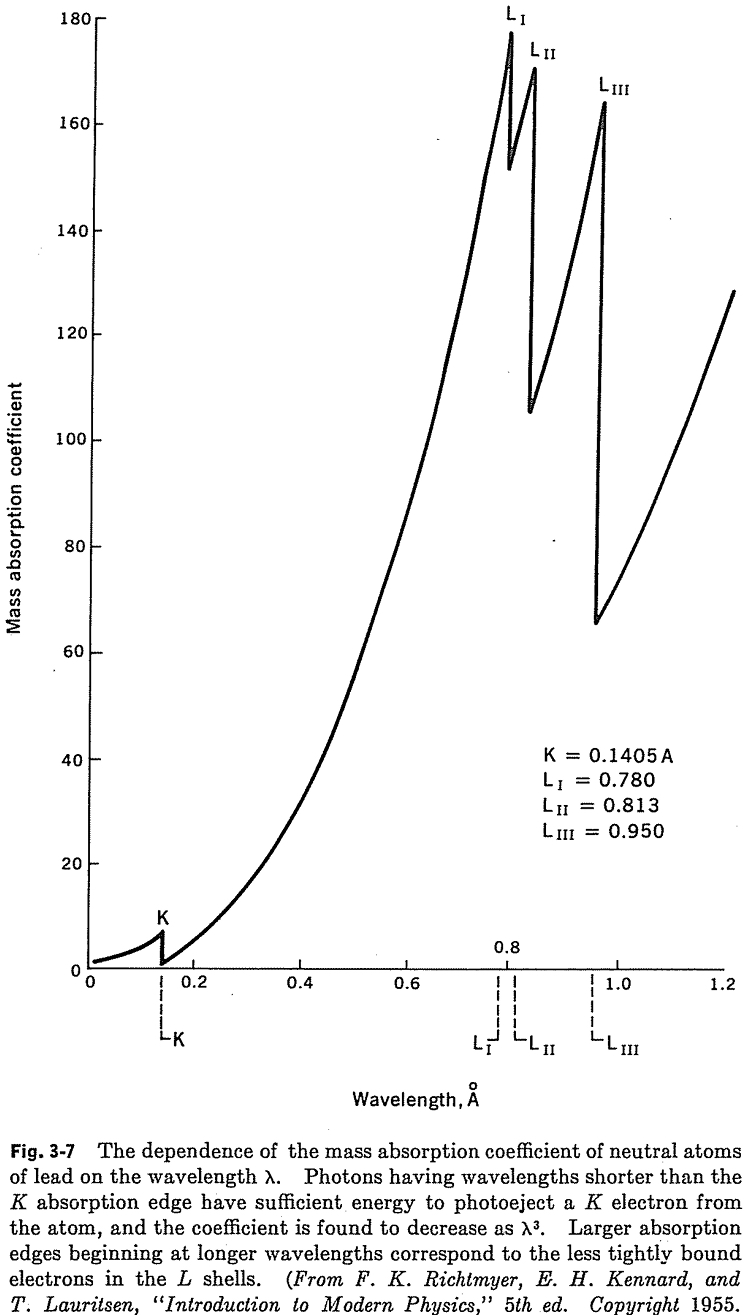
\includegraphics[trim={0.0cm 0cm 0.0cm 0},clip, keepaspectratio,width=0.95\textwidth]{BF-abs}\label{fig:BF-abs}
			\end{figure}
        \end{column}
    \end{columns}
    \begin{align*}
        &\psi_k=L^{-\frac{3}{2}}\Exp{i\scap{k}{r}}, E_k=\frac{\hbar^2k^2}{2m}: \Delta n= \frac{L^3\Delta p_x\Delta p_y\Delta p_z}{h^3}=\frac{L^34\pi p^2\,dp}{h^3}, \frac{\Delta n}{\Delta E}=\frac{m^{\frac{3}{2}}\sqrt{E}L^3}{\sqrt{2}\pi^2\hbar^2}
    \end{align*}
    
    \begin{align*}
        &\frac{\Delta n}{\Delta\omega}=\frac{d\Omega}{4\pi}\frac{m^{\frac{3}{2}}\sqrt{E}L^3}{\sqrt{2}\pi^2\hbar^2}\\
        &\psi_s=R_{1s}Y_{00}=\frac{1}{\sqrt{\pi}}(\frac{Z}{a})^{\frac{3}{2}}\exp {-\frac{Zr}{a}}\tag{photoejection from K-shell}\\
        &\TDy{\Omega}{\sigma(\omega)}=\frac{32\alpha\hbar k(\hat{e}\cdot\vec{k})^2}{m\omega}(\frac{Z}{a})^5(\frac{Z^2}{a^2}+q^2)^{-4}, q=\vec{k}-\frac{\omega}{c}\hat{n}\tag{$\hbar q$ momentum transfer - agree with obs for $\hbar\omega\gg\chi$}
    \end{align*}
    \begin{columns}[T]
        \begin{column}{0.7\textwidth}
                $\theta$: photon direction/ejected electron dir,$\psi$:polarization/plane photon and electron momenta
            \begin{align*}
                &(\frac{Z}{a})^2+q^2=(\frac{Z}{a})^2+k^2+(\frac{\omega}{c})^2-2k\frac{\omega}{c}\cos{\theta}=2 \frac{m\omega}{\hbar}(1-\frac{\hbar k}{mc}\cos{\theta}+\frac{\hbar\omega}{2mc^2})\\
                &\frac{\hbar^2k^2}{2m}=\hbar\omega-\chi=\hbar\omega-\frac{Z^2e^2}{2a}\tag{energy conservation}\\
                &\TDy{\Omega}{\sigma(\omega)}=2\alpha k(\hat{e}\cdot\vec{k})^2(\frac{\hbar}{m\omega})^5(\frac{Z}{a})^5(1-\beta\cos{\theta})^{-4}\tag{\Pelectron v is NR, ignore photon energy vs \Pelectron rest-mass en.}\\
                &=2\alpha k^3(\frac{\hbar}{m\omega})^5(\frac{Z}{a})^5 \frac{\sin^2{\theta}\cos^2{\phi}}{(1-\beta\cos{\theta})^4}: \sigma(\omega)\approx \frac{8\pi\alpha}{3}(\frac{Z}{a})^5(\frac{\hbar}{m\omega})^5k^3\\
                &\sigma(\hbar\omega\gg\chi)\approx \frac{2}{3}\frac{\alpha^{\frac{9}{2}}}{\pi^{\frac{5}{2}}a^{\frac{3}{2}}}Z^5\lambda^{\frac{7}{2}}\tag{High freq approx: $k^2\approx \frac{2m\omega}{\hbar}$}\\
                &\lambda^{\frac{7}{2}}\approx\lambda^3\lambda_k^{\frac{1}{2}},\frac{hc}{\lambda_k}=\frac{Z^2e^2}{2a}\Rightarrow Z^5\lambda^{\frac{7}{2}}\propto Z^4\lambda^3\tag{Near edge: wrong approx/right behaviour}
            \end{align*}
        \end{column}
        \begin{column}{0.3\textwidth}
            \begin{figure}[!ht]
                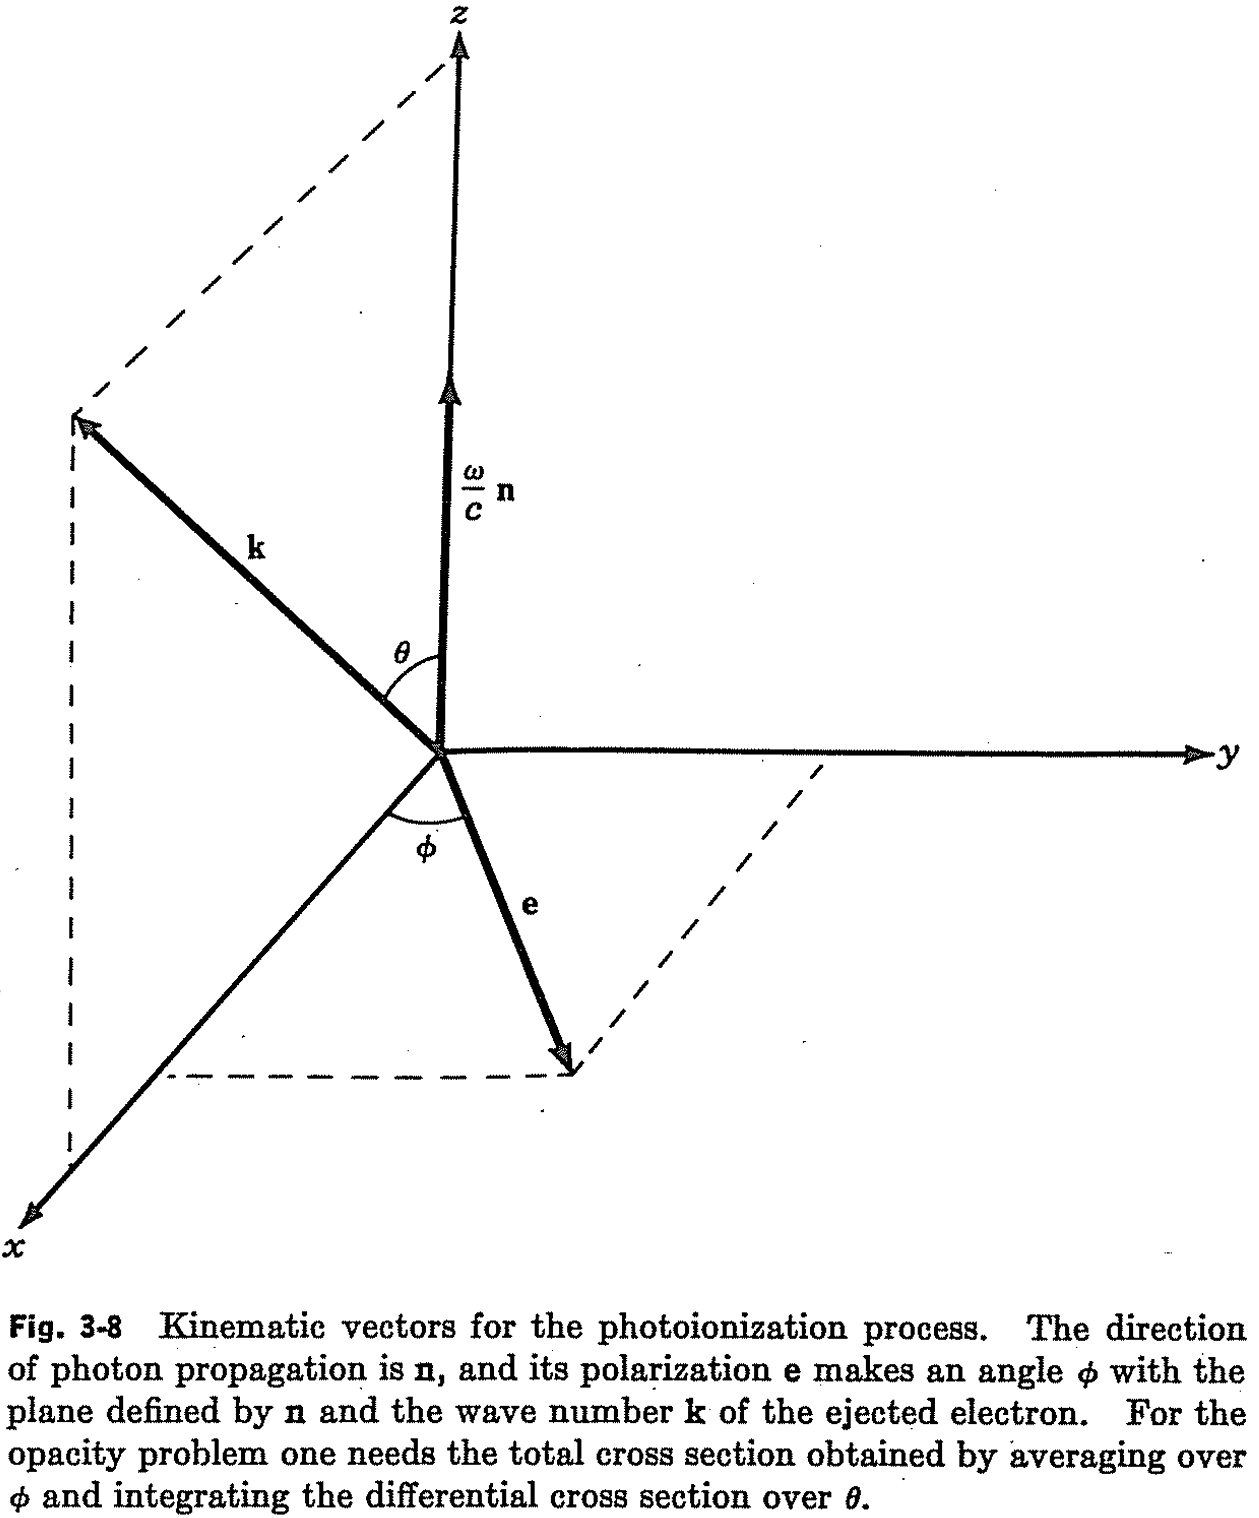
\includegraphics[trim={0.0cm 0cm 0.0cm 0},clip, keepaspectratio,width=0.95\textwidth]{photoejection-kin}\label{fig:photoejection-kin}
			\end{figure}
        \end{column}
    \end{columns}
    
\end{frame}

\begin{frame}{BF absorption: most important frequencies near edge $\hbar\omega\approx\chi$}
    Replacing free-electron wave function by plane wave (Born Approx) is inadequate near threshold where electron wavefunction is strongly perturbed by Coulomb interaction: these are the most important frequencies for stellar opacity problem we have to use exact Coulomb waves for $\psi_k$:
    \begin{align*}
        &\sigma_{BF}=\frac{64\pi^4me^{10}}{3\sqrt{3}ch^6}\frac{Z^4}{n^5}\frac{g(\nu,n,l,Z)}{\nu^3}=\num{2.82e29}\frac{Z^4}{n^5\nu^3}g(\nu,n,l,Z)\si{\square\cm}
    \end{align*}
\end{frame}

\subsection{FF opacity}

\begin{frame}{FF Absorption: Inverse bremsstrahlung}
    \begin{columns}[T]
        \begin{column}{0.65\textwidth}
    \begin{align*}
        &\frac{p_k^2}{2m}=\frac{p_s^2}{2m}+\hbar\omega, H_{tot}=H_{free}+V_c+H_{int}\tag{Heavy Z absorbs negl. kin ener.}
    \end{align*}
    \begin{itemize}
        \item If we take unpert. $H_0=H_f+V_c$, zeroth order wave function $\psi_k^{(0)}$ are coulomb wf - \Pelectron scattering by ion. Perturbation at first order in interaction with em field.
    \item Born Approx: $H_0=H_{free}$, 0th order wf are plane waves, perturbed H is $V_c+V_{int}$. Transition probability propto $|V_{ks}|^2$ if is null $V_{ks}\to\sum_m \frac{V_{km}V_{ms}}{E_s-E_m}$ - virtual transition $s\to m \to k$ (energy don't have to be conserved as m has short lifetime). Two possibility: 1) Electron absorbs photon ($H_{int}$) and its momentum becomes $\vec{k}_m=\vec{k}_s+\frac{\omega}{c}\hat{n}$ then $V_c$ causes scattering transition $\vec{k}_m\to\vec{k}_k$. 2) $V_c$ causes transition $\vec{k}_s\to\vec{k}_m$, such that $H_{int}$ has a momentum conserving matrix element for absorption of photon: $\vec{k}_k=\vec{k}_m+\frac{\omega}{c}\hat{n}$. The sum is on both intermediate states.
        \end{itemize}
        \end{column}
        \begin{column}{0.35\textwidth}
            \begin{figure}[!ht]
                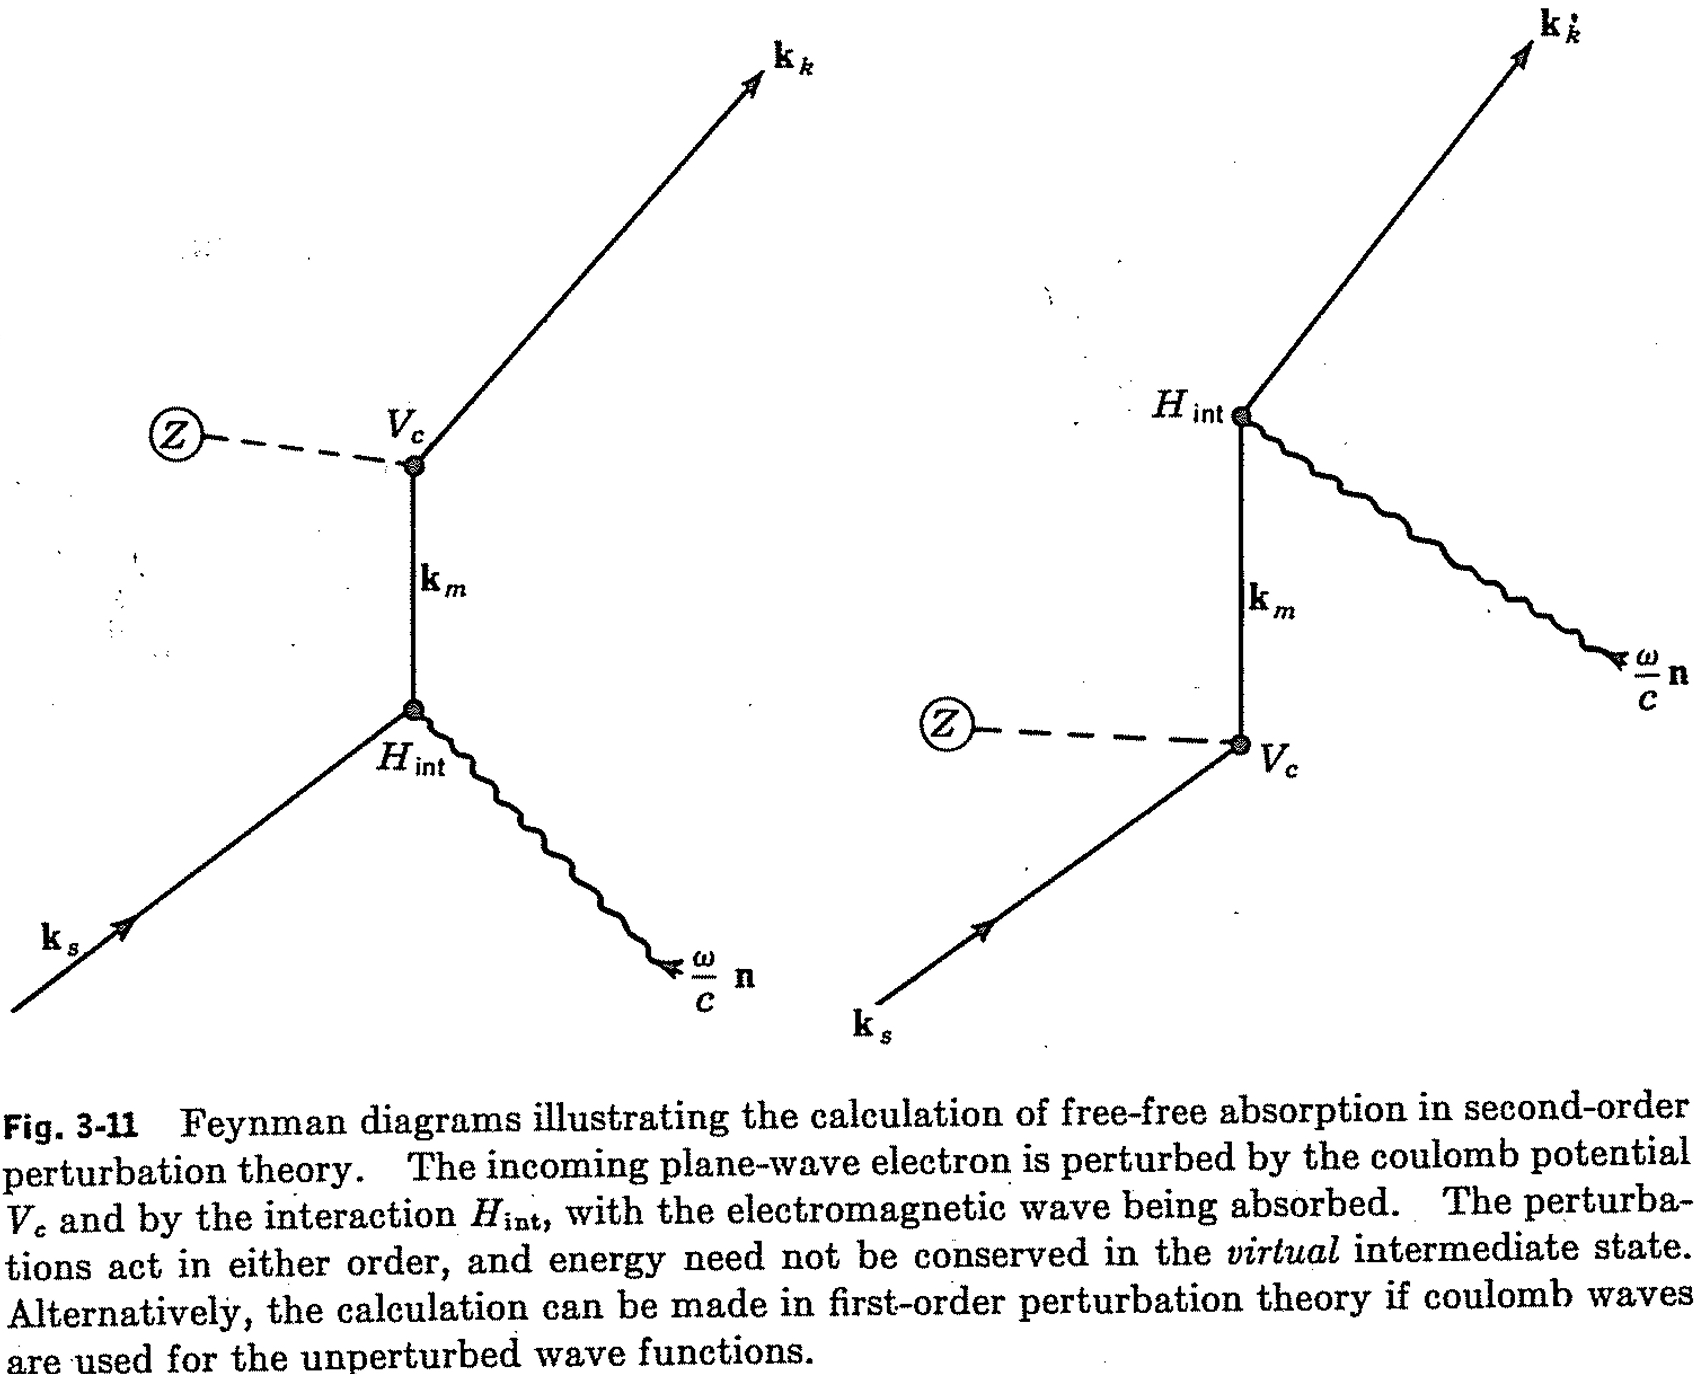
\includegraphics[trim={0.0cm 0cm 0.0cm 0},clip, keepaspectratio,width=0.95\textwidth]{FF-feynman}\label{fig:FF-feynman}
			\end{figure}
        \end{column}
    \end{columns}
    \begin{align*}
        &r=\frac{2\pi}{\hbar}|\sum_m \frac{V_{km}V_{ms}}{E_s-E_m}|^2\rho(E_k)\tag{$\rho$ density of final states - GoldenRules: transition prob per unit time}\\
        &d\sigma_{ff}(Z,\nu,v)=\frac{4\pi Z^2e^6g_{ff}(v,\nu)}{3\sqrt{3}hcm^2v\nu^3}n_e(v)\,dv\tag{$n_e(v)$ \Pelectron density with $[v,v+dv]$ }\\
        &n_e(v)dv=4\pi n_e(\frac{m}{2\pi kT})^{\frac{3}{2}}\Exp{-\frac{mv^2}{2kT}}v^2\,dv, \bar{\sigma}_{ff}(Z,\nu)=\int_0^{\infty}d\sigma(Z,\nu,v):\\
        &\bar{\sigma}_{ff}(Z,\nu,T)=\num{3.69e8}\frac{Z^2n_e\bar{g}_{ff}}{T^{\frac{1}{2}}\nu^3}\si{\cm}\Rightarrow\kappa_{ff}(\nu)=\sum \frac{X_zN_0}{A_z}\bar{\sigma}_{ff}(Z,\nu)
    \end{align*}
\end{frame}

\begin{frame}{Rosseland Mean for FF opacity - Kramer's op.: $\propto\rho T^{-3.5}$}
    FF opacity dominate total opacity in important regions of $\rho$-T plane
    \begin{columns}[T]
        \begin{column}{0.65\textwidth}
            \begin{align*}
                &u=\frac{h\nu}{kT}: \frac{1}{\kappa}=\frac{2\pi k^4}{ac^3h^3}\int_0^{\infty}\frac{u^4\exp{2u}}{\kappa(u)[\exp{u}-1]^3}\,du\tag{all true abs}\\
                &\kappa_{ff}(\nu)\approx K\nu^{-3}=K(\frac{h}{kT})^3u^{-3}, \exv{g_{ff}}\approx\bar{g}_{ff}(u_{max}(=7))\tag{ignoring deps g on $\nu$}\\
                &\Rightarrow \frac{1}{\kappa}=\frac{1}{K\exv{\nu^{-3}}}, \exv{\nu^{-3}}\approx[197(\frac{kT}{h})^3]^{-1}:(h\nu)_{eff}\approx5.82kT\\
                &\exv{\sigma_{ff}}=\num{2.07e-25}\frac{Z^2n_e}{T^{3.5}}\bar{g}_{ff}(u=7)\si{\square\cm}=\num{1.25e-1}\frac{Z^2\bar{g}_{ff}}{\mu_e}\frac{\rho}{T^{3.5}}\si{\square\cm}\\
                &\approx\num{6.25e-2}(1+X)Z^2\bar{g}_{ff}\rho T^{-3.5}\si{\square\cm}\\
                &\Rightarrow\exv{\kappa_{ff}}=\num{7.53e22}\frac{\rho}{\mu_eT^{3.5}}\sum_Z \frac{Z^2\bar{g}_{ff}(Z,u=7)X_Z}{A_Z}\si{\square\cm\per\gram}
            \end{align*}
        \end{column}
        \begin{column}{0.35\textwidth}
            \begin{figure}[!ht]
                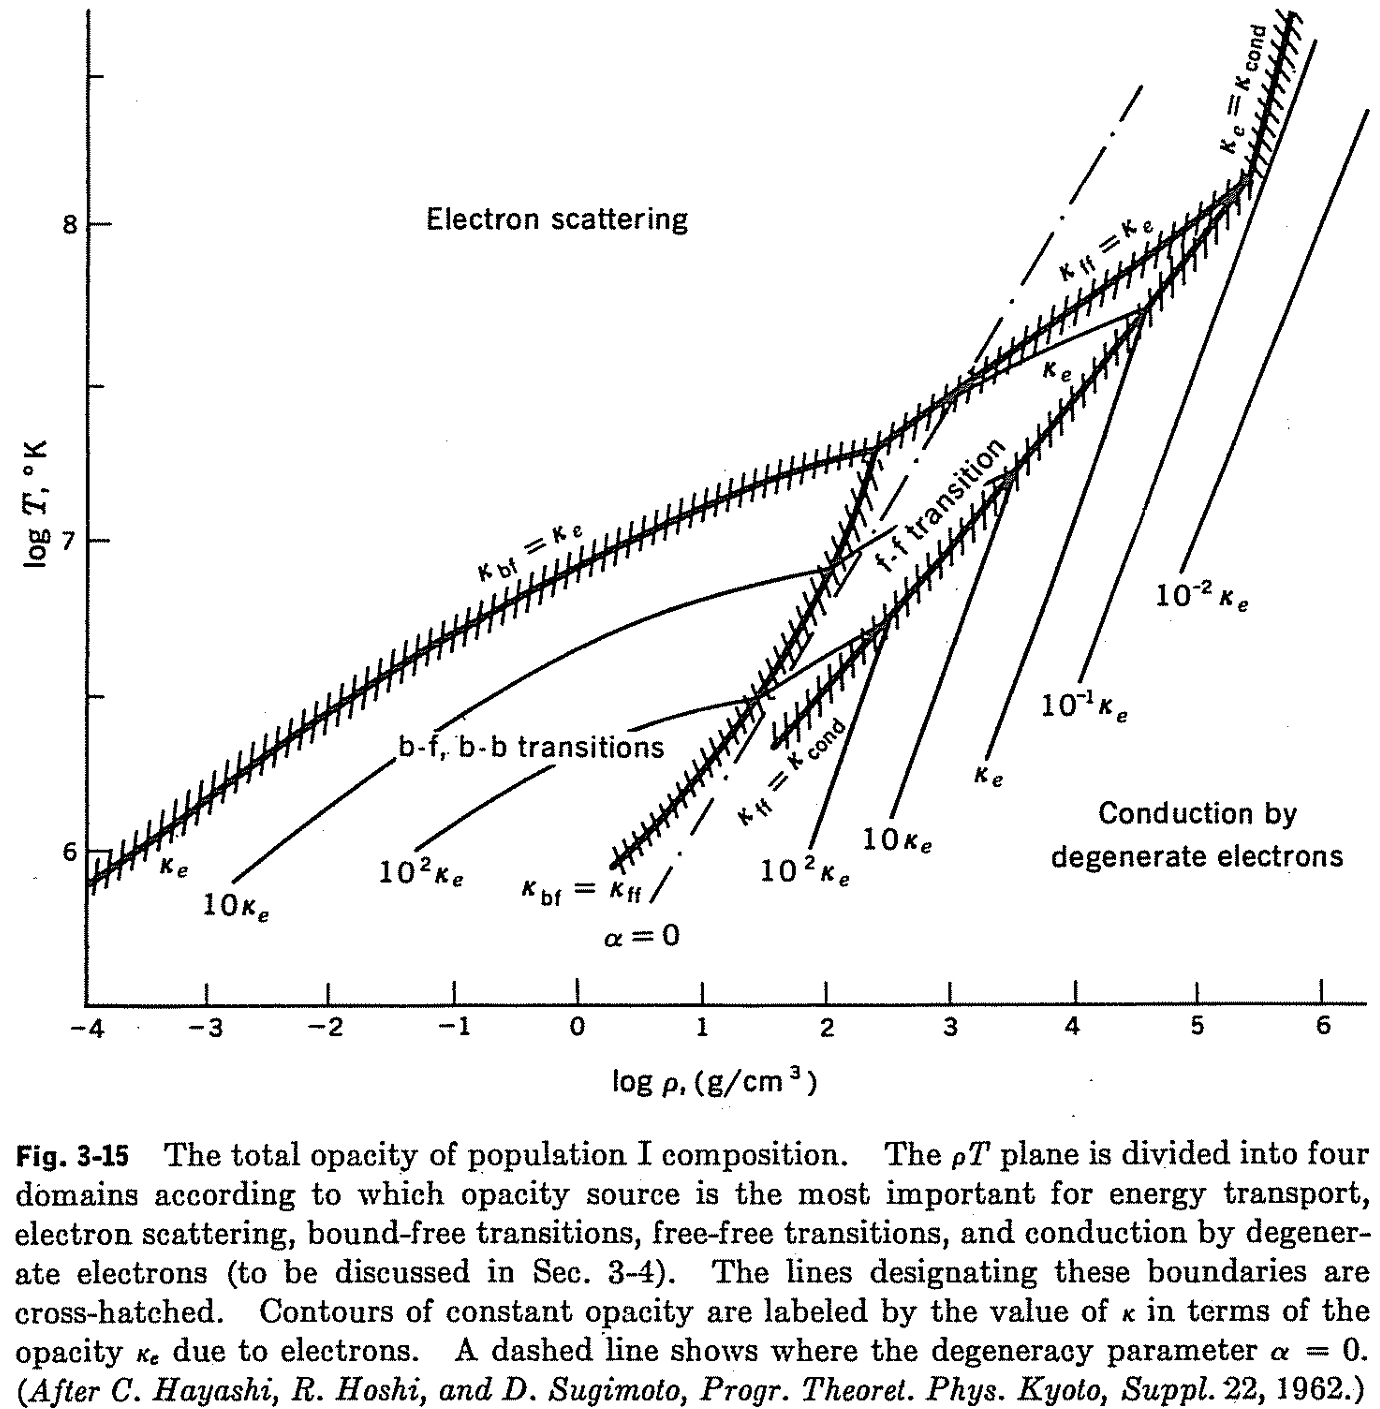
\includegraphics[trim={0.0cm 0cm 0.0cm 0},clip, keepaspectratio,width=0.95\textwidth]{rhoTplane-kappa}\label{fig:rhoTplane-kappa}
			\end{figure}
        \end{column}
    \end{columns}
    
\end{frame}

\subsection{Electron opacity}

\begin{frame}{Scattering of photons by free electrons}
    Scattering opacity by free lectrons so small that is dominated by BF opacity until ionization is complete and by FF opacity until T is suff. great: in high T range electron scattering is main opacity source. In quantum electrodyn. vector potential $\vec{A}$ is expanded linearly  in terms of creation/destruction operators for single photons - the term $\scap{p}{A}$ in BF, FF, BB gives rise to single photon absorption - but matrix element for scattering must involve destruction of initial photon/creation of scattered: must be quadratic in vector potential $\vec{A}$.
            \begin{align*}
                &H_{int}=\frac{e}{mc}\scap{p}{A}+\frac{e^2}{2mc^2}\scap{A}{A}=H_{int}^{(1)}+H_{int}^{(2)}: \braket{k|H_{int}|s}=\sum_m \frac{\braket{k|H^{(1)|m}\braket{m|H^{(1)}_{int}|s}}}{E_s-E_m}+\braket{k|H^{(2)}_{int}|s}\propto e^2
            \end{align*}
            \begin{columns}[T]
        \begin{column}{0.65\textwidth}
            second order part of $H^{(1)}_{int}$ and hitherto neglected $H_{int}^{(2)}$ - for photon's $E\ll m_ec^2$ answer con be obtained from classical EM. When free electron is invested by EM radiation accelerates so radiates in direction other than incident (scattering), for photon energy $\ll m_ec^2$ scattering radiation has same freq as incident. Power radiated into solid angle $d\Omega$ at angle $\psi$ to direction of accel $\vec{a}$ for NR particles: $dP=\frac{e^2}{4\pi c^3}a^2\sin^2{\psi}\,d\Omega$, scattered waves are pol in plane of $\vec{a}$ and in viewer dir. ($\sin^2{\psi}=1-\sin^2{\theta}\cos^2{\phi}$)
            \begin{align*}
                &\vec{E}(z,t)=\hat{\epsilon}E_0\cos{(kz-\omega t)}\Rightarrow\vec{a}=-\hat{\epsilon}\frac{e}{m}E_0\cos{(kz-\omega t)}\\
                &\bar{a^2}=\frac{1}{2}\frac{e^2}{m^2}E_0^2:\TDy{\Omega}{P}=\frac{e^2}{4\pi c^3}\frac{1}{2}\frac{e^2}{m^2}E_0^2\sin^2{\psi}=\frac{c}{8\pi}E_0^2(\frac{e^2}{mc^2})^2\sin^2{\psi}\\
                &\TDy{\Omega}{\sigma}=\frac{\text{power radiated/unit solid angle}}{\text{incident power/unit area}}, S=\frac{\text{power}}{\text{area}}=\frac{c}{4\pi}\bar{E^2}=\frac{c}{8\pi}E_0^2:\\
                &\TDy{\Omega}{\sigma}=(\frac{e^2}{mc^2})^2\sin^2{\psi}(\propto (H_{int}^{(2)}))^2\\
                &r_0=\frac{e^2}{mc^2}=\SI{2.818e-13}{\cm}\tag{$r_0$ radius of shell charge e of energy $m_ec^2$}
            \end{align*}
        \end{column}
        \begin{column}{0.35\textwidth}
            \begin{figure}[!ht]
                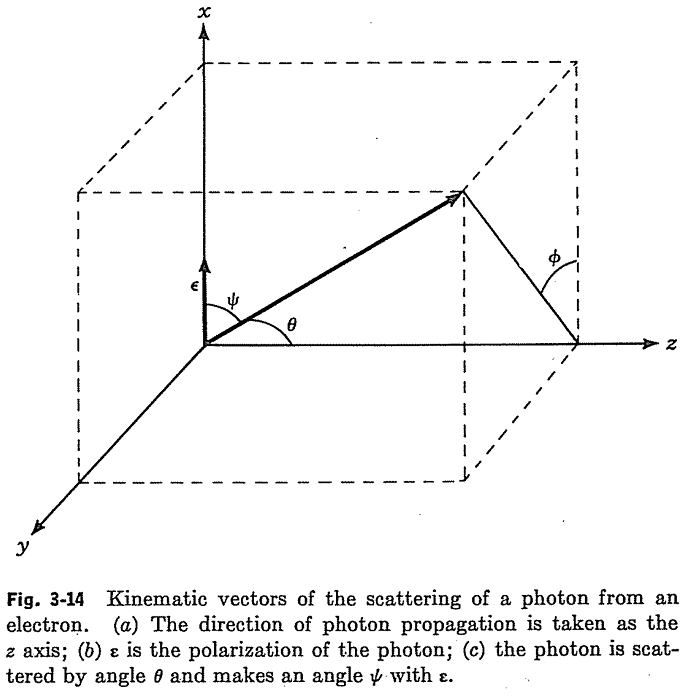
\includegraphics[trim={0.0cm 0cm 0.0cm 0},clip, keepaspectratio,width=0.75\textwidth]{kappa-electronscattering-kin}\label{fig:kappa-electronscattering-kin}
                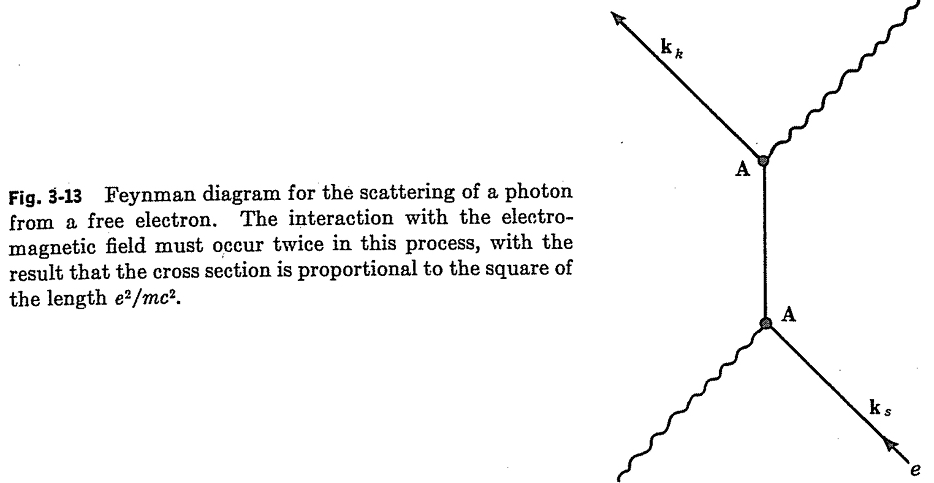
\includegraphics[trim={0.0cm 0cm 0.0cm 0},clip, keepaspectratio,width=0.9\textwidth]{kappa-electronscattering-diag}\label{fig:kappa-electronscattering-diag}
			\end{figure}
        \end{column}
    \end{columns}
    
\end{frame}

\begin{frame}{Thomson and Klein-Nishina crosssection}
    \begin{columns}[T]
        \begin{column}{0.6\textwidth}
            \begin{align*}
                &\overline{\sin^2{\psi}}=1-\sin^2{\theta}\overline{cos^2{\phi}}=1-\frac{1}{2}\sin^2{\theta}\tag{unpol.}\\
                &\TDy{\Omega}{\sigma}=(\frac{e^2}{mc^2})^2 \frac{1}{2}(1+\cos^2{\theta})\tag{Thomson}\\
                &d\sigma=\frac{8\pi}{3}(\frac{e^2}{mc^2})^2p(\cos{\theta})\frac{d\Omega}{4\pi}\tag{Norm. scat. phase function}\\
                &=\sigma_T[p(\cos{\theta})\frac{d\Omega}{4\pi}],\sigma_T=\frac{8\pi}{3}(\frac{e^2}{mc^2})^2=\SI{0.665e-24}{\square\cm}\\
                &\kappa_{es}=\frac{0.4}{\mu_e}\approx0.2(1+X_H)\tag{complete ioniz.}\\
                &
            \end{align*}
        \end{column}
        \begin{column}{0.4\textwidth}
            Thomson: not valid for rel. energy or $E_{\gamma}\geq mc^2$ ($T>\SI{e9}{\kelvin}$) - $\TDy{\Omega}{\sigma}\propto \frac{1}{m^2}$ so electron scatterin far more important than scattering from nuclei.
            Other type of scattering occurs in cooler part of stars - Rayleigh scattering, by from ions (harmonically bounded electrons) and molecules where ionization is incomplete. In He-H gas ionized electron scattering opacity dominate FF only if $T>\num{4.5e6}\rho^{0.286}$. Scattering phase function propto $1+\cos^2{\theta}$ cancellation made in diffusion theory of rad-transf is satisfied.
        \end{column}
    \end{columns}
    Klein-Nishina formula: when photon energy becomes sign. fraction of $mc^2$, $\epsilon=\frac{h\nu}{mc^2}$
    \begin{align*}
        &d\sigma=\frac{d\Omega}{4\pi}\frac{\sigma_T \frac{3}{4}(1+\cos^2{\theta})}{(1+2\epsilon\sin^2{\frac{\theta}{2}})}[1+\frac{4\epsilon^2\sin^4{\frac{\theta}{2}}}{(1+\cos^2{\theta})(1+2\epsilon\sin^2{\frac{\theta}{2}})}]\\
        &\sigma=\frac{3}{4}\sigma_T\{\frac{1+\epsilon}{\epsilon^2}[\frac{2+2\epsilon}{1+2\epsilon}-\frac{\ln{(1+2\epsilon)}}{\epsilon}]+\frac{\ln{(1+2\epsilon)}}{2\epsilon}-\frac{1+3\epsilon}{(1+2\epsilon)^2}\}
    \end{align*}
    At high temperature $\sigma<\sigma_T$, scattering phase function contains odd power of $\cos{\theta}$ (scattering of photons into/out no longer cancels), energy of scattered photon is reduced in prop to $\frac{\Delta\nu}{\nu}\approx \frac{h\nu}{mc^2}$.
    High energy photons may create \Pelectron\APelectron pair in nucleus's field: $\gamma+Z\to Z+\APelectron+\Pelectron$ if $h\nu>2mc^2$, $\sigma_{pair}\approx Z^2\num{e-3}\sigma_T$ (not important opacity source, but created electron increase scatterers and its annihilation produce neutrinos).
\end{frame}

\section{Radiative transfer equation}

\begin{frame}{Derivation of transfer equation}
    \begin{columns}[T]
        \begin{column}{0.3\textwidth}
\begin{figure}[!ht]
	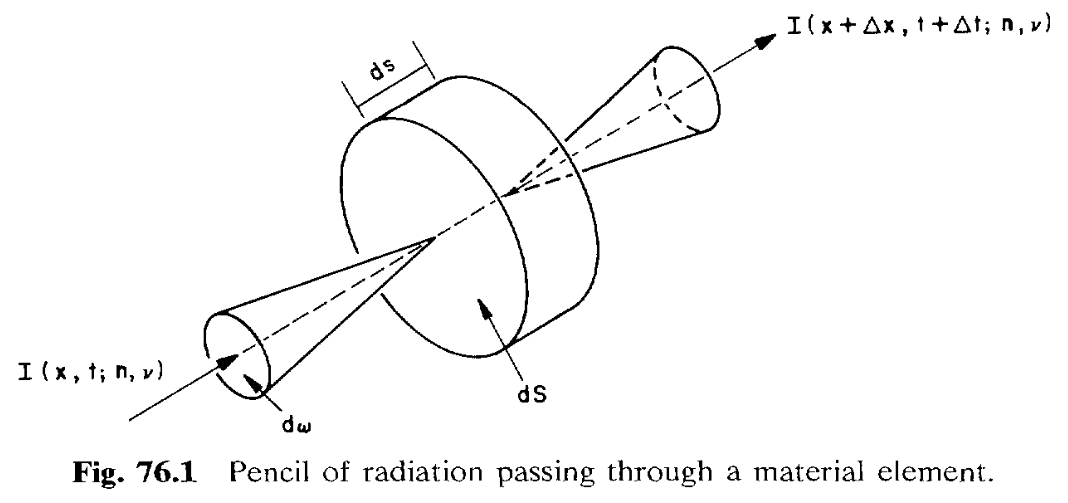
\includegraphics[trim={0cm 0cm 1cm 0cm},clip, keepaspectratio,width=0.99\textwidth]{radthroughcyl}
\end{figure}
        \end{column}
        \begin{column}{0.7\textwidth}
\begin{align*}
    &\Delta t=\frac{ds}{c}:\ I(\vec{x}+\Delta\vec{x},t+\Delta t;\vec{n},\nu)\\
    &=I(\vec{x},t;\vec{n},\nu)+[\frac{1}{c}\PDy{t}{I}]\,ds
\end{align*}
        \end{column}
    \end{columns}
  \begin{align*}
   &I(\vec{x}+\Delta\vec{x},t+\Delta t;\vec{n},\nu)-I(\vec{x},t;\vec{n},\nu)=[\eta(\vec{x},t;\vec{n},\nu)-\chi(\vec{x},t;\vec{n},\nu)I(\vec{x},t;\vec{n},\nu)]ds\,dS\,d\Omega\,d\nu\,dt&\\
   &[\frac{1}{c}\PDof{t}+\nabla_{\vec{s}}]I(\vec{x},t;\vec{n},\nu)=\eta(\vec{x},t;\vec{n},\nu)-\chi(\vec{x},t;\vec{n},\nu)I(\vec{x},t;\vec{n},\nu)&\tag{Trans. eq.}\\
   &[\frac{1}{c}\PDof{t}+\mu\PDof{z}]I(z,t;\mu,\nu)=\eta(z,t;\mu,\nu)-\chi(\ldots)I(\ldots)&\tag{1D planar}
  \end{align*}

  \begin{columns}[T]
      \begin{column}{0.15\textwidth}
          \begin{figure}[!ht]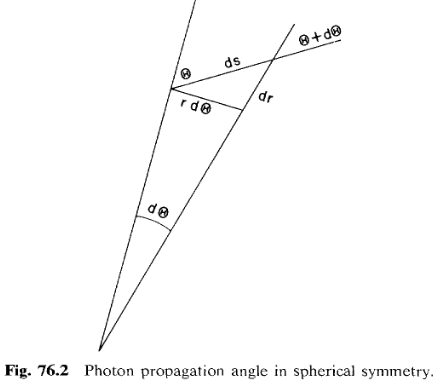
\includegraphics[trim={2cm 0cm 1cm 5mm},clip, keepaspectratio,width=0.99\textwidth]{radtransfspheric}\label{fig:}\end{figure}
      \end{column}
      \begin{column}{0.85\textwidth}
          \begin{align*}
          &dr=\cos{\Theta}\,ds=\mu\,ds,\ r\,d\Theta=-\sin{\Theta}\,ds=-\sqrt{1-\mu^2}\,ds&\tag{spherical sym}\\
          &\PDof{s}=\PDy{s}{r}\PDof{r}+\PDy{s}{\Theta}=\mu\PDof{r}+\frac{(1-\mu^2)}{r}\PDof{\mu}&\\
          &[\frac{1}{c}\PDof{t}+\mu\PDof{r}+\frac{(1-\mu^2)}{r}\PDof{\mu}]I(r,t;\mu,\nu)=\eta(r,t;\mu,\nu)-\chi(r,t;\mu,\nu)I(r,t;\mu,\nu)&
          \end{align*}
      \end{column}
  \end{columns}
  Classical, macroscopic, phenomenological: not included polarization, dispersion, coherence, interference and quantum effects.
\end{frame}

\begin{frame}{Einstein relations}
    \begin{columns}[T]
        \begin{column}{0.5\textwidth}
            Radiative transition $i\to j$: $h\nu_{ij}=\epsilon_j-\epsilon_i$, stat. weight $g_i, g_j$, \keyword{absorption probability $B_{ij}$}, \keyword{spontaneus emission probability $A_{ji}$}: isotropic
                        \[\dot{E}_{\nu}=\frac{A_{ji}h\nu_{ji}}{4\pi}n_i\phi_{\nu}\]
                \begin{align*}
                &(\frac{n_i}{n_j})^*B_{ij}I_{\nu}^*=A_{ji}+B_{ji}I_{\nu}^*\label{CR and TE}\\
                                &(\frac{n_j}{n_i})^*=\frac{g_j}{g_i}\exp{-h\nu/KT}\\
                            &\Rightarrow B_{\nu}=\frac{A_{ji}}{B_{ji}}\invers{[\frac{g_iB_{ij}}{g_jB_{ji}}\exp{h\nu_{ij}kT}-1]}\\
                        &g_iB_{ij}=g_jB_{ji}\tag{Atomic prop $\to$ E. coeff}\\
                    &A_{ji}=\frac{2h\nu_{ij}^3}{c^2}B_{ji}\tag{also for non TE}
            \end{align*}
        \end{column}
        \begin{column}{0.5\textwidth}
            Number of photons absorbed per unit volume per unit time:
            \[r_{ij}=n_i\phi_{\nu}B_{ij}I_{\nu}(\frac{d\Omega}{4\pi})d\nu\]
            \keyword{Induced emission probability $B_{ji}$}: rate of stimulated energy emission per unit volume (as $I_{\nu}$)
            \[\dot{E}_{\nu}=\frac{B_{ji}h\nu_{ij}}{4\pi}n_i\phi_{\nu}I_{\nu}\]
            \keyword{Line emission/absorption ceff} (co-moving frame):
            \begin{align*}
    &\eta_l(\nu)=n_j\frac{A_{ji}h\nu_{ij}}{4\pi}\phi_{\nu}\\
    &\chi_l(\nu)=\frac{n_iB_{ij}h\nu_{ij}}{4\pi}[1-\frac{g_in_j}{g_jn_i}]\phi_{\nu}
            \end{align*}
        \end{column}
    \end{columns}
    \begin{columns}[T]
        \begin{column}{0.4\textwidth}
             Source function for a line: ratio emissivity to opacity:
        \end{column}
        \begin{column}{0.6\textwidth}
            \[S_l=\frac{n_jA_{ji}}{n_iB_{ij}-n_jB_{ji}}=\frac{2h\nu_{ij}^3}{c^2}\invers{[\frac{g_jn_i}{g_in_j}-1]}\to B_{\nu}\]
        \end{column}
    \end{columns}
\end{frame}

\begin{frame}{Einstein-Milne relations}
    \begin{columns}[T]
        \begin{column}{0.55\textwidth}
            Fluid frame; $n_e(v)$ maxwellian - prob. ionization by rad $(\nu,\nu+d\nu)$: Energy absorption coeff. $\alpha_{\nu}=h\nu p_{\nu}$,
            photoionization rate: $n_0h\nu I_{\nu}\,d\nu$, $n_0$ atoms number density, $n_1$ density of ions - $F(v)$/$G(v)$ spontaneous/induced recombination prob for \Pelectron with $(v,v+dv)$, recombination rate: $n_1n_e(v)[F+GI]vdv$
        \end{column}
        \begin{column}{0.45\textwidth}
            Thermodynamic equilibrium: photoionizations equal recombinations
            \begin{align*}
                &n_0^*p_{\nu}B_{\nu}=n_1^*n_e(v)[F(v)+G(v)B_{\nu}]\\
                &\Rightarrow B_{\nu}=\frac{F(v)}{G(v)}\invers{(\frac{n_0^*p_{\nu}m_e}{n_1^*n_e(v)hG(v)}-1)}\\
                &\left\{\begin{array}{l}F(v)=\frac{2h\nu^3}{c^2}G(v)\\\frac{p_{\nu}}{G(v)}\frac{h}{m}[n_2(v)(\frac{n_1}{n_0})^*]\exp{h\nu/kT}\\
                \end{array}\right.\tag{1}
            \end{align*}
        \end{column}
    \end{columns}
    \begin{align}
        &n_e(v)\,dv=n_e[\frac{m_e}{2\pi kT}]^{3/2}\exp{-\frac{1}{2}\frac{mv^2}{kT}}4\pi v^2\,dv\tag{TE: $n_e$ maxwell.}\\
        &(\frac{n_1}{n_0})^*=(\frac{g_0}{2g_1})[\frac{h^2}{2\pi m_ekT}]^{3/2}\exp{\epsilon_{ion}/kT}=n_e\phi_0\tag{Saha eq.}\\
        &\Rightarrow p_{\nu}=\frac{8\pi m^2v^2g_1}{h^2g_0}G(v)=\frac{4\pi c^2m^2v^2g_1}{h^3g_0\nu^3}F(v)\tag{2}
    \end{align}
 (1)-(2) continuum analog of Einstein relations   
\end{frame}

\begin{frame}{Continuum emission/absorption coeff.}
    \begin{align*}
        &\kappa_{\nu}=h\nu[n_0p_{\nu}-\frac{h}{m}n_1n_e(v)G(v)]=[n_0-n_0^*\exp{-\frac{h\nu}{kT}}]\alpha_{\nu}\\
        &\kappa_{\nu}^*=n_0^*\underbrace{[1-\exp{-\frac{h\nu}{kT}}]}_{\text{correction stimulated emission}}\alpha_{\nu}\tag{LTE}
    \end{align*}
    Recombination (spontaneous/induced) results from ion-electrons collision: if they have Maxwellian distribution, recombination at LTE rate whereas for lines rate depends on upper level population - Spontaneous continuum emission coeff.:
\begin{align*}
    &\eta_{\nu}^t=h\nu n_1n_e(v)F(v)\frac{h}{m}=\frac{hn_1n_e(v)F(v)}{m_ep_{\nu}}\alpha_{\nu}\\
    &\to\frac{2h\nu^3}{c^2}n_0^*\alpha\exp{-\frac{h\nu}{kT}}=n_0^*(1-\exp{-\frac{h\nu}{kT}})\alpha_{\nu}B_{\nu}(T)=\kappa_{\nu}^*B_{\nu}(T)
\end{align*}
\end{frame}

\begin{frame}{Absorption, emission and scattering}
    \begin{itemize}
        \item \keyword{Total absorption coef $\chi(\vec{x},t;\hat{n},\nu)$}: material volume of cross section $dS$ and length $dl$ removes energy from beam in interval dt:
            \[\delta=\chi(\ldots)I(\ldots)dld\Omega d\nu dt\]
            Sum over all states that can absorb at $\nu$ of the product of occupation number of those states (\si{\per\cubic\cm}) times their atomic crosssection (\si{\square\cm}) at that freq.: $\lambda_{\nu}=\invers{\chi_{\nu}}$ is mean free path of photons
        \item \keyword{Doppler Shift}: Photons moving along $\hat{n}$ with freq. $\nu$ in Lab. frame, has in fluid frame of materials moving at $\vec{v}$ freq. $\nu_0=\nu[1-\frac{\vec{v}\cdot\hat{n}}{c}]$ ($\frac{\Delta\nu_D}{\nu_0}c=13(\frac{T}{\SI{e4}{\kelvin}})^{1/2}\si{\kilo\meter\per\second}$).
        \item \keyword{Emission coeff. (Emissivity)}: $\eta(\vec{x},t;\hat{n},\nu)$ such that an element $dS\,dl$ add energy to beam
            \[\delta E=\eta(\ldots)dldSd\Omega\,dVdt\ [\si{\erg\per\cubic\cm\per\second\per\hertz\per\ster}]\]
        \item \keyword{Scattering}: Photon excites atoms then atoms decay into fundamentals - Photons collides with free electrons (Thopson scattering), atom or molecule in which they excite a resonance (Rayleigh/Raman scattering) 
    \end{itemize}
\end{frame}

\begin{frame}{Kirchoff-Plank relation}
    In TE: $(\eta_{\nu}^t)^*=(\kappa_{\nu}I_{\nu})^*$, $*$ indica TE dove $I_{\nu}=B_{\nu}$ quindi $(\eta_{\nu}^t)^*=(\kappa_{\nu}B_{\nu})^*$ - when gradients of physical quantities are small over photon destruction lenght: LTE
\end{frame}

\begin{frame}{Thermodynamics of adiabat enclosed rad: Kirchoff-Plank rel.}
    \begin{block}{Einstein coeff.}
Radiative transition $i\to j$: $h\nu_{ij}=\epsilon_j-\epsilon_i$, stat. weight $g_i, g_j$, \keyword{absorption probability $B_{ij}$}, \keyword{spontaneus emission probability $A_{ji}$}: isotropic
            \[\dot{E}_{\nu}=\frac{A_{ji}h\nu_{ji}}{4\pi}n_i\phi_{\nu}\]
            \begin{align*}
                &(\frac{n_i}{n_j})^*B_{ij}I_{\nu}^*=A_{ji}+B_{ji}I_{\nu}^*\label{CR and TE}\\
                &(\frac{n_j}{n_i})^*=\frac{g_j}{g_i}\exp{-h\nu/KT}\\
                &\Rightarrow B_{\nu}=\frac{A_{ji}}{B_{ji}}\invers{[\frac{g_iB_{ij}}{g_jB_{ji}}\exp{h\nu_{ij}kT}-1]}\\
                &g_iB_{ij}=g_jB_{ji}\tag{Atomic prop $\to$ E. coeff}\\
                &A_{ji}=\frac{2h\nu_{ij}^3}{c^2}B_{ji}\tag{also for non TE}
            \end{align*}
   \end{block}
   \begin{block}{E. of transfer in star interior}
       \begin{align}
        &\TDy{s}{I_{\nu}}\frac{1}{\rho}=j_{\nu}-\kappa_{\nu}I_{\nu}\Leftrightarrow\TDy{s}{I_{\nu_{nm}}}=N_n(A_{nm}+B_{nm}I_{\nu_{nm}})h\nu_{nm}-N_mB_{mn}h\nu_{nm}I_{\nu_{nm}}\label{ERT}
    \end{align}
    \begin{columns}[T]
        \begin{column}{0.3\textwidth}
            $I_{\nu}$ in isotropic homogeneous medium adiabat. enclosed deps only on T:
        \end{column}
        \begin{column}{0.7\textwidth}
        \begin{align*}
        \frac{1}{\rho}\TDy{s}{I_{\nu}}=0\Rightarrow j_{\nu}=\kappa_{\nu}I_{\nu}\Rightarrow I_{\nu_{nm}}=\frac{N_nA_{nm}}{N_mB_{mn}-N_nB_{nm}}\label{Kirckoff-Plank}
\end{align*}
        \end{column}
    \end{columns} 
   \end{block}
\end{frame}
\begin{frame}{Scattering of radiation in spectral line}
    \begin{itemize}
    \item Broadened atomic level can be decomposed into sublevels and transition between these sublevels can be treated statistically: \keyword{redistribution function}: probability in atom's frame that incoming photon of freq $\nu'$ is scattered as outgoing $\nu$.
    \item Semiclassical picture
    \item Natural population of levels: probability emitting photon $(\hat{n},\nu)$ in transition to lower level averaged over ensemble of identical atoms is independent of previous history of ensemble (not naturally populated by radiative processes in which there is correlation with prop. prev. absorbed/emitted photon: stimulated emission)
\item Distro of individual sublevel of naturally popul. n at $E_n$: $L(\chi,\gamma)=\frac{\gamma}{\pi(\chi^2+\gamma^2)}$, $\chi=\frac{E-E_n}{h}$, $2\gamma_n=\sum_{m<n}A_{nm}+\sum_{m\neq n}B_{nm}\bar{J}_{nm}+R_{n\kappa}+\sum_{n\neq m}C_{nm}+C_{n\kappa}+Q_n$, A,B bb Einstein coeff., R photoion rate, C coll rate (bb,bf), $Q_n$ effective rate of elastic coll.in level n, $\bar{J}_{nm}=\int_0^{\infty}\oint \frac{d\Omega}{4\pi}\phi_{nm}(\nu,\hat{n})\,d\nu$ freq-averaged mean intensity for $n\to m$ (suppose spont em coeff much bigger than induced em coeff)
\item Atom's frame absorption profile for transition between broadened level $i\to e$: $\phi_{ie}(\nu')=\intsinf{}L(\chi_i,\gamma_i)L(\chi_e',\gamma_e)\,d\chi_i$; $L(\chi_i,\gamma_i)$ natural occupation probability of sublevels in $(\chi_i,\chi_i+\,d\chi_i)$, $L(\chi_e'=\nu'-\nu_{ie}+\chi_i,\gamma_e)$ is occupation prob of level e when photon $\nu'$ is absorbed, total prob of transition is product summed over all i states, Cauchy's residue theorem $\phi_{ij}(\nu')=L(\nu'-\nu_{ij},\gamma_{ij})=\frac{\gamma_{ij}}{\pi[(\nu'-\nu_{ij})^2+\gamma_{ij}^2]}$, $\gamma_{ij}=\gamma_i+\gamma_j$
\end{itemize}
\end{frame}

\begin{frame}{Semiclassical picture of photon scattering}
    
\end{frame}

\begin{frame}{True absorption and scattering coeff.}
    True absorption plus scattering $\chi=\kappa+\sigma$, thermal emission plus scattering emission $\eta=\eta^T+\eta^S$ - if $\sigma_l$ (line scattering cross section) is isotropic total energy removed from beam is
    \begin{align*}
        &\sigma(\ldots)\intzi\,d\nu_0'\phi(\vec{x},t;\nu_0')\oint\,d\Omega_0'I_0(\vec{x},t;\hat{n}_0',\nu_0')\\
        &=4\pi\sigma_l(\vec{x},t)\intzi\phi(\vec{x},t;\nu_0')J_0(\vec{x},t;\nu_0')d\nu_0'
    \end{align*}
    Prob. absorption of photon with $(\hat{n}',\nu')$ absorbed and re-emitted on $(\hat{n},\nu)$ is $R(\hat{n}',\nu',\hat{n},\nu)$.
    If photons are random in angle and along line profile (\keyword{complete redistribution}: good approx. in many cases, within Doppler core of a line, if excited atoms suffer many collisions before re-emission) the fluid frame/lab. frame emission(emissivity) by scattering is
    \begin{align*}
        &\eta_0^S(\vec{x},t;\nu_0)=\sigma(\ldots)\phi(\vec{x},t;\nu_0)\intzi\,d\nu_0'\phi(\vec{x},t;\nu_0')J_0(\vec{x},t;\hat{n}_0',\nu_0')\\
        &\eta^S(\vec{x},t;\hat{n},\nu_0)=\sigma(\ldots)\phi(\vec{x},t;\nu_0)\intzi\,d\nu_0'\oint\,d\Omega\phi(\vec{x},t;\nu_0')I_0(\vec{x},t;\hat{n}_0',\nu_0')
    \end{align*}
    When scattering is isotropic and coherent the emissivity is $\eta_0^S=\sigma_0(\vec{x},t)J_0(\vec{x},t;\nu_0)$: Thompson scattering of continuum photons by free electrons
\end{frame}

  \begin{frame}{Total Opacity and Total Emission coeff. and LTE}
      \begin{align*}
              &\chi_{\nu}=\kappa_{\nu}+\sigma_{\nu}=\underbrace{\sum_i\sum_{j>i}[n_i-\frac{g_i}{g_j}n_j]\alpha_{ij}(\nu)}_{\text{BB - line}}+\underbrace{\sum_i(n_i-n_i^*\exp{-\frac{h\nu}{kT}})\alpha_{ik}(\nu)}_{\text{BF}}\\
                      &+\underbrace{\sum_{\kappa}n_en_{\kappa}\alpha_{\kappa\kappa}(\nu,T)(1-\exp{-\frac{h\nu}{kT}})}_{\text{FF}}+\underbrace{n_e\sigma_e}_{\text{Thompson scatt. by free e}}\tag{Tot.Opa.}\\
          &\eta_{\nu}^{th}=\frac{2h\nu^3}{c^2}[\sum_i\sum_{j>i}n_j \frac{g_i}{g_j}\alpha_{ij}(\nu)+\sum_in_i^*\alpha_{i\kappa}(\nu)\exp{-\frac{h\nu}{kT}}+\sum_{\kappa}n_en_{\kappa}\alpha_{\kappa\kappa}(\nu,T)\exp{-\frac{h\nu}{kT}}]\\
                  &\xrightarrow{LTE}\frac{2h\nu^3}{c^2}\exp{-\frac{h\nu}{kT}}[\sum_in_i^* (\sum_{j>i}\alpha_{ij}(\nu)+\alpha_{i\kappa}(\nu))+\sum_{\kappa}n_en_{\kappa}\alpha_{\kappa\kappa}(\nu,T)\exp{-\frac{h\nu}{kT}}]\\
                          &\Rightarrow\chi_{\nu}^*=\kappa_{\nu}^*+n_e\sigma_e,\ (\eta_{\nu}^{th})^*=\kappa_{\nu}^*B_{\nu}
          \end{align*}
          \end{frame}

\section{Solution of RE in far interior}


\begin{frame}{Total Opacity and Total Emission coeff. and LTE}
    \begin{align*}
        &\chi_{\nu}=\kappa_{\nu}+\sigma_{\nu}=\underbrace{\sum_i\sum_{j>i}[n_i-\frac{g_i}{g_j}n_j]\alpha_{ij}(\nu)}_{\text{BB - line}}+\underbrace{\sum_i(n_i-n_i^*\exp{-\frac{h\nu}{kT}})\alpha_{ik}(\nu)}_{\text{BF}}\\
        &+\underbrace{\sum_{\kappa}n_en_{\kappa}\alpha_{\kappa\kappa}(\nu,T)(1-\exp{-\frac{h\nu}{kT}})}_{\text{FF}}+\underbrace{n_e\sigma_e}_{\text{Thompson scatt. by free e}}\tag{Tot.Opa.}\\
        &\eta_{\nu}^{th}=\frac{2h\nu^3}{c^2}[\sum_i\sum_{j>i}n_j \frac{g_i}{g_j}\alpha_{ij}(\nu)+\sum_in_i^*\alpha_{i\kappa}(\nu)\exp{-\frac{h\nu}{kT}}+\sum_{\kappa}n_en_{\kappa}\alpha_{\kappa\kappa}(\nu,T)\exp{-\frac{h\nu}{kT}}]\\
        &\xrightarrow{LTE}\frac{2h\nu^3}{c^2}\exp{-\frac{h\nu}{kT}}[\sum_in_i^* (\sum_{j>i}\alpha_{ij}(\nu)+\alpha_{i\kappa}(\nu))+\sum_{\kappa}n_en_{\kappa}\alpha_{\kappa\kappa}(\nu,T)\exp{-\frac{h\nu}{kT}}]\\
        &\Rightarrow\chi_{\nu}^*=\kappa_{\nu}^*+n_e\sigma_e,\ (\eta_{\nu}^{th})^*=\kappa_{\nu}^*B_{\nu}
    \end{align*}
\end{frame}


\section{Fusione nucleare}\linkdest{reactionrates}

\begin{frame}{Rate of nuclear reaction}
    \begin{columns}[T]
        \begin{column}{0.5\textwidth}
            \begin{align*}
                &\sigma=\frac{\#\text{ interaction per T}}{\# \text{ incident per A per T}*\#\text{ target within beam}}\\
                &=\frac{N_R/T}{N_{beam}/(AT)N_T}\Rightarrow \frac{N_R}{T}=\frac{N_{beam}}{TA}N_T\sigma\\
                &j_{beam}=\frac{N_{beam}}{TA},\ \SI{1}{\barn}=\SI{e-24}{\square\cm},\ \SI{1}{\square\femto\meter}=\SI{e-2}{\barn}\\
                &r_{01}=\frac{N_0N_1\exv{\sigma v}}{1+\delta_{01}},\ m_{01}=\frac{m_0m_1}{m_0+m_1}\\
                &P(v)\,dv=(\frac{m_{01}}{2\pi KT})^{\frac{3}{2}}\exp{-\frac{m_{01}v^2}{2KT}}4\pi v^2\,dv\\
                &=P(E)\,dE=\frac{2}{\sqrt{\pi}}\frac{\sqrt{E}}{(KT)^{\frac{3}{2}}}\exp{-\frac{E}{KT}}\,dE
            \end{align*}
            If velocity of 0,1 are sep. Maxwell. also $v_{01}$ is Maxwell.;$K\approx\SI{8.6e-5}{\ev\per\kelvin}$
        \end{column}
        \begin{column}{0.5\textwidth}
            \begin{align*}
                &\frac{N_R}{VT}=(\sigma N_T)(\frac{N_b}{VAT})\\
                &=\sigma \frac{N_T}{V}\frac{N_b}{AT}=\sigma \frac{N_T}{V}v \frac{N_b}{V}\\
                &r_{01}=N_0N_1\sigma v\xrightarrow{P(v)}N_0N_1\exv{\sigma v}_{01}\\
                &N_0N_1\tag{Pairs number density: non id.}\\
                &\frac{N_0(N_0-1)}{2}\to \frac{N_0^2}{2}\tag{Number density pairs: id}\\
                &v_T=\sqrt{\frac{2KT}{m_{01}}}\tag{Peak $P(v)$}\\
                &E_T=\frac{KT}{2}\tag{Peak $P(E)$}
            \end{align*}
            $N_0$, $N_1$ number density
        \end{column}
    \end{columns}
    \begin{block}{Reaction rate at high temperature: we have to consider excited states}
        \begin{align*}
        &P_{i\mu}=\frac{N_{i\mu}}{N_i}=\frac{g_{i\mu}\exp{-\frac{E_{i\mu}}{KT}}}{\sum_{\mu}g_{i\mu}\exp{-\frac{E_{i\mu}}{KT}}}=\frac{g_{i\mu}\exp{-\frac{E_{i\mu}}{KT}}}{G_i}\tag{$E_{i\mu}$ excitation energy}\\
        &N_A\exv{\sigma v}^*_{01\to23}=\sum_{\mu}P_{0\mu}\sum_{\nu}N_A\exv{\sigma v}^{\mu\to\nu}_{01\to23}\tag{$\mu$ states target 0, $\nu$ in 3}\\
        &=R_{tt}N_A\exv{\sigma v}_{01\to23}\tag{$R_{tt}$ stellar enhancement factor}
    \end{align*}
    \end{block}
\end{frame}

\begin{frame}{Photodisintegration ($\gamma+3\to0+1$)}
    Most astrophys. photodisin $\gamma+3\to0+1$ are derived from corresp. particle induced reaction rate applying reciproc. theorem but some are measured directly:
    \begin{align*}
        &j_b=\frac{N_b}{AT}=\frac{cN_b}{V}\Rightarrow r_{\gamma3}=\frac{N_R}{VT}=N_3N_{\gamma}c\sigma(E_{\gamma}),\ N_3=\frac{N_T}{V},\ N_{\gamma}=\frac{N_b}{V}\tag{$\gamma3\to01$}\\
        &r_{\gamma3}=N_3\int_0^{\infty}cN_{\gamma}(E_{\gamma})\sigma(E_{\gamma})\,dE_{\gamma}\tag{If $Q_{\gamma3\to01}<0$ integration lower limit is $E_t=Q_{01\to\gamma3}$}\\
        &N_{\gamma}(E_{\gamma})\,dE_{\gamma}=\frac{u(E_{\gamma})}{E_{\gamma}}\,dE_{\gamma}=\frac{8\pi}{(hc)^3}\frac{E_{\gamma}^2}{\exp{\frac{E_{\gamma}}{KT}}-1}\,dE_{\gamma},\ u(E_{\gamma})\,dE_{\gamma}=\frac{8\pi}{(hc)^3}\frac{E_{\gamma}}{\exp{\frac{E_{\gamma}}{KT}-1}},\ u(\nu)\,d\nu=\frac{8\pi}{(hc)^3}\frac{1}{\exp{\frac{E_{\gamma}}{KT}}-1}\,d\nu\\
        &\lambda_{\gamma}(3)=\frac{r_{\gamma3}}{N_3}=\int_0^{\infty}cN_{\gamma}(E_{\gamma})\sigma(E_{\gamma})\,dE_{\gamma}\Rightarrow\lambda_{\gamma}(3)=\frac{8\pi}{h^3c^2}\int_0^{\infty}\frac{E_{\gamma}^2\sigma(E_{\gamma})}{\exp{\frac{E_{\gamma}}{KT}}-1}\tag{decay const}\\
        &\frac{\sigma_{\gamma3\to01}}{\sigma_{01\to\gamma3}}=\frac{(2j_0+1)(2j_1+1)}{2(2j_2+1)}\frac{2m_{01}c^2E_{01}}{E_{\gamma}^2}\frac{1}{(1+\delta_{01})}\tag{forward/reverse}\\
        &\Rightarrow \frac{8\pi m_{01}}{h^3}\frac{(2j_0+1)(2j_1+1)}{(2j_3+1)}\int_0^{\infty}\overbrace{\frac{E_{\gamma}-Q_{01\to\gamma3}}{\exp{\frac{E_{\gamma}}{KT}-1}}}^{E_{01} \text{Kinetic energy in COM}}\sigma_{01\to\gamma3}\,dE_{\gamma}\\
    &\lambda_{\gamma}(3)\approx\int_0^{\infty}(E_{\gamma}-Q_{01\to\gamma3})\exp{-\frac{E_{\gamma}}{KT}}\frac{\exp{-2\pi\eta}}{E_{01}}S(E_{01})\,dE_{\gamma}\tag{charged particle em., $E_{\gamma}\gg KT$, $S\approx\const{}$}\\
    &\approx S(E_0)\exp{-\frac{Q_{01\to\gamma3}}{KT}}\int_0^{\infty}\exp{-2\pi\eta}\exp{-\frac{E_{01}}{KT}}\,dE_{01},\ E_{\gamma}^{eff}=E_0+Q_{01\to\gamma3}\tag{$E_0$ Gamow peak forward reaction}\\
    &\lambda_{\gamma}(3)\propto\int_0^{\infty}(E_{\gamma}-Q_{01\to\gamma3})\exp{-\frac{E_{\gamma}}{KT}}E_{01}^{l-1/2}\,dE_{\gamma}\tag{$(\gamma,n)$: small $E_n$: $\sigma_{n\gamma}\propto\sigma_l\propto E^{l-1/2}$, $E_{\gamma}^{eff}\approx E_{thr}$}\\
    &\approx\int_0^{\infty}\exp{-\frac{E_{\gamma}}{KT}}(E_{\gamma}-Q_{01\to\gamma3})^{l+1/2}\,dE_{\gamma},\ E^{eff}_{\gamma}=(l+\frac{1}{2})KT+Q_{n\gamma}\tag{n-capt.: $E_n^{eff}=(l+\frac{1}{2})KT$ so $E_{\gamma}^{eff}=(l+\frac{1}{2})KT+Q_{n\gamma}$}
    \end{align*}
\end{frame}

\begin{frame}{Resonance reaction rate}
    Narrow Res.: One level Breit-Wigner formula
            \begin{itemize}
                \item Isolated: Level density in compound nucleus is small so resonance do not overlap
                \item Narrow: Partial width cont. over total res. width ($\Gamma<\text{few kev}$)
            \end{itemize}
            \begin{align*}
                &\sigma_{BW}(E)=\frac{\lambda^2}{4\pi}\frac{(2J+1)(1+\delta_{01})}{(2j_0+1)(2j_1+1)}\frac{\Gamma_a\Gamma_b}{(E_r-E)^2+\Gamma^2/4}
            \end{align*}
            $j_i$ Spin of target/projectile, $J,E_R$ spin and energy of resonance, $\Gamma_i,\Gamma$ Partial width of entrance/exit channel, total res width.
            \begin{align*}
                &N_A\exv{\sigma v}=\sqrt{\frac{8}{\pi m_{01}}}\frac{N_A}{(KT)^{\frac{3}{2}}}\int_0^{\infty}E\sigma_{BW}(E)\exp{-\frac{E}{KT}}\,dE=N_A \frac{\sqrt{2\pi}\hbar^2}{(m_{01}KT)^{\frac{3}{2}}}\omega\int_0^{\infty}\frac{\Gamma_a\Gamma_b\exp{-\frac{E}{KT}}}{(E-E_R)^2+\Gamma^2/4}\,dE\\
                &\omega=\frac{(2J+1)(1+\delta_{01})}{(2j_0+1)(2j_0+1)}
            \end{align*}
            Narrow res.: MB factor $\exp{-\frac{E}{KT}}$ and $\Gamma_i$ approx const.:
            \begin{equation*}
            N_A\exv{\sigma v}=N_A(\frac{2\pi}{m_{01}KT})^{\frac{3}{2}}\hbar^2\exp{-\frac{E_r}{KT}}\omega\gamma 
            \end{equation*}
            $\omega\gamma=\omega \frac{\Gamma_a\Gamma_b}{\Gamma}$, proportional to area under resonance cross-section (ie product of max. cross-section $\sigma_{BW}(E_r)=\frac{\lambda_r^2}{\pi}\omega \frac{\Gamma_a\Gamma_b}{\Gamma}$ and total res. width): $\Gamma*\sigma_{BW}(E_r)=\frac{\lambda_r^2}{\pi}\omega\gamma$. Several narrow res. add incoherently.
            Temperature deps.: $N_A\exv{\sigma v}_T=N_A\exv{\sigma v}_{T_0}(\frac{T}{T_0})^{\num{11.605}\frac{E_r}{T_9}-\frac{3}{2}}$, $E_r$ in \si{\mega\ev}: T sensitive increases as \xdiminuisce{T} and \xaumenta{E_r}.
            Broad Res.: Explicit energy dependence of cross-section
            \begin{align*}
                &N_A\exv{\sigma v}=\sqrt{2\pi}\frac{N_A\omega\hbar^2}{(m_{01}KT)^{\frac{3}{2}}}\int_0^{\infty}\exp{-\frac{E}{KT}}\frac{\Gamma_a(E)\Gamma_b(E+Q-E_f)}{(E_r-E)^2+\Gamma(E)^2/4}
            \end{align*}
            $\Gamma_b$ has to be calculated at energy $E_{23}=E_{01}+Q_{01\to23}-E_f$.
\end{frame}

\begin{frame}{Reaction Rate Equilibrium}
    \begin{align*}
        &r=r_{01\to23}-r_{23\to01}=\frac{N_0N_1\exv{\sigma v}_{01to23}}{(1+\delta_{01})}-\frac{N_2N_2\exv{\sigma v}_{23\to01}}{(1+\delta_{23})}\tag{Equilibrium $r=0$}\\
        &\frac{N_2N_3}{N_0N_1}=\frac{(1+\delta_{23})\exv{\sigma v}_{01\to23}}{(1+\delta_{01})\exv{\sigma v}_{23\to01}}=\frac{(2j_2+1)(2j_3+1)}{(2j_0+1)(2j_1+1)}\frac{G_2^{norm}G_3^{norm}}{G_0^{norm}G_1^{norm}}(\frac{m_{23}}{m_{01}})^{\frac{3}{2}}\exp{\frac{Q_{01\to23}}{KT}}\\
        &G_i^{norm}=\frac{G_i}{g_i}=\frac{\sum_{\mu}g_{i\mu}\exp{-\frac{E_{i\mu}}{KT}}}{g_i}\tag{Normalized partition function, $g_i$ stat. weight ground state of nucleus i}\\
        &r=0=r_{01\to\gamma3}-r_{\gamma3\to01}=\frac{N_0N_1\exv{\sigma v}_{01\to\gamma3}}{(1+\delta_{01})}-\lambda_{\gamma}(3)N_3\tag{$01\to\gamma3$}\\
        &\frac{N_3}{N_0N_1}=\frac{1}{(1+\delta_{01})}\frac{\exv{\sigma v}_{01\to\gamma3}}{\lambda_{\gamma}(3)}=\frac{1}{1+\delta_{01}}\frac{1}{N_1}\frac{\lambda_1(0)}{\lambda_{\gamma}(3)}\\
        &=(\frac{h^2}{2\pi})^{\frac{3}{2}}\frac{1}{(m_{01}KT)^{\frac{3}{2}}}\frac{(2j_3+1)}{(2j_0+1)(2j_1+1)}\frac{G_3^{norm}}{G_0^{norm}G_1^{norm}}\exp{\frac{Q_{01\to\gamma3}}{KT}}\tag{Saha statistical equation}\\
            &01\to23\tag{$0$,$3$: Heavy, $1$, $2$: $\alpha$, \Pproton, \Pneutron}\\
            &\left.\TDy{t}{N_0}\right|_{01\to23}=-r_{01\to23},\ \left.\TDy{t}{N_3}\right|_{23\to01}=-r_{23\to01}\\
                    &f_{03}=|\TDy{t}{N_0}|_{01\to23}-\TDy{t}{N_3}|_{23\to01}|=|r_{01\to23}-r_{23\to01}|=|N_0N_1\exv{\sigma v}_{01\to23}-N_2N_3\exv{\sigma v}_{23\to01}|\tag{Net abundance flow between 0,3}\\
                    &(\TDy{t}{N_0})_{01\to23}\approx(\TDy{t}{N_3})_{23\to01}\gg f_{03}\approx0\ \phi_{03}=\frac{|r_{01\to23}-r_{23\to01}|}{\max{r_{01\to23},r_{23\to01}}}\approx0\tag{equilibrium condition}
                            \end{align*}
        A differenza di stato stazionario, la condizione di equilibrio non implica $N_0,N_3$ costanti: refers to near equality of forward/reverse abundance flow between pair nuclei; when a group of severals pairs comes into equilibrium the resulting solution of reaction network is of quasi-equilibrium (Arnett96).
\end{frame}

\begin{frame}{Sezione d'urto fusion nucleare}
    \begin{itemize}
        \item Sezione d'urto: $\sigma(E)=\pi\lambdabar^2*P_0(E)*S(E)$, $E$ l'energia cinetica nel centro di massa dei nuclei. Prodotto sezione d'urto geometrica (nel riferimento del CM: $\sigma\approx\sum_{l=0}^{\frac{R}{\lambdabar}}(2l+1)\pi\lambdabar^2=\pi(R+\lambdabar)^2$ - per energie tipiche interni stellari approx onda S), della probabilit\'a di attraversamento della barriera coulombiana $P_0$ e del fattore astrofisico $S(E)$. \todo{$R\ll\lambdabar$??}
            La lunghezza d'onda di de Broglie relativa delle particelle descrive l'indeterminazione sulla posizione nell'urto di due particelle con momento relativo p $\lambdabar=\frac{\hbar}{p}=\frac{\hbar}{\sqrt{2mE}}$: $\pi\lambdabar^2\propto \frac{1}{p^2}\propto \frac{1}{E}$; geometrical cross-section for \si{\kilo\ev} nucleons $\pi\lambdabar^2=657\invers{E}\si{\barn}$ where E is in \si{\kilo\ev} and reduced mass in amu.
\item Probability crossing coulomb barrier: $\widehat{T}=\widehat{T}_1\ldots\widehat{T}_n\approx\exp{[-\frac{2}{\hbar}\sqrt{2m(V_i-E)}(R_{i+1}-R_i)]}\xrightarrow{n large}\exp{[-\frac{2}{\hbar}\int_{R_0}^{R_c}\sqrt{2m[V(r)-E]}\,dr]}$. The leading term of expansion of $\widehat{T}$ for $\frac{E}{V_C}\ll1$: $\widehat{T}\approx\exp{(-\frac{2\pi}{\hbar}\sqrt{\frac{m}{2E}Z_0Z_1e^2})}=\Exp{-2\pi\eta}=P_0(E)$. Sommerfeld parameter $\eta$, numerically $2\pi\eta=\num{0.989534}Z_0Z_1\sqrt{\frac{1}{E}\frac{M_0M_1}{M_0+M_1}}$, $M_i$ in units of u.
\item Astrophysical factor $S(E)$: $S(E)=\sigma(E)E\exp{\frac{2\pi Z_1Z_0e^2}{\hbar v}}$.
    Slow variation with E (non resonant case): expansion around $E=0$ $S(E)=S(0)+S'(0)E+\frac{2}{2}S''(0)E^2$ is suff.
    \begin{equation*}
        N_A\exv{\sigma v}=(\frac{4}{3})^{\frac{3}{2}}\frac{\hbar}{\pi}\frac{N_A}{m_{01}Z_0Z_1e^2}S_{eff}\tau^2\exp{-\tau}
    \end{equation*}
    $\tau=\frac{3E_0}{KT}$, $S_{eff}$ accounts for energy dependence of astrophysical factor and asymmetry of Gamow Peak
\item Gamow peak - Gauss Approx. $\PDof{E}[\frac{2\pi}{\hbar}\sqrt{\frac{m_{01}}{2E}Z_0Z_1e^2-\frac{E}{KT}}]_{E_0}=0=\PDof{E}(\frac{E}{KT}+bE^{-\frac{1}{2}})_{E_0}=\frac{1}{KT}-\frac{1}{2}bE_0^{-\frac{3}{2}}$:
    \begin{align*}
        &\exp{(-\frac{E}{KT}-bE^{-\frac{1}{2}})}\approx C\exp{-(\frac{E-E_0}{\Delta/2})^2},\ \Delta=\frac{4}{\sqrt{3}}\sqrt{E_0KT}=\num{0.75}(Z_0^2Z_1^2AT_6^5)^{\frac{1}{6}}\si{\kilo\ev}\tag{match 2nd der}\\
        &E_0=(\frac{bKT}{2})^{\frac{2}{3}}=[(\frac{\pi}{\hbar})^2(Z_0Z_1e^2)^2(\frac{m_{01}}{2})(KT)^2]^{\frac{1}{3}}=\num{0.1220}(Z_0^2Z_1^2\frac{M_0M_1}{M_0+M_1}T_9^2)
    \end{align*}
\end{itemize}

\end{frame}

\begin{frame}{Coulomb screening and continuum depression}
    In ionized plasma electron are attracted to nuclei while nuclei repel each others:each nucleus is surrounded by charged cloud, so Coulomb barrier in nuclear reaction becomes thinner increasing tunneling probability and reaction rate.
    L'energia potenziale dovuta all'interazione di due nuclei $Z_1$ e $Z_2$ a distanza r contiene un contributo delle altre cariche presenti nel plasma
    \begin{equation*}
    U=\frac{Z_1Z_2e^2}{r}+U_s(r_{12})
    \end{equation*}
    l'energia potenziale non schermata e contributo della nuvola elettronica: $U_s$ aumenta la probabilit\'a di attraversamento della barriera coulombiana.
    Fattore moltiplicativo: $f=\exp{-\midfrac{U_0}{KT}}$ dove $U_0=U_s(0)$ poich\'e $r\ll r_D$ e considerando solo la correzione al fattore di penetrazione ($E_G\gg U_0$).

Per determinare $U_0$ considero l'energia potenziale di $Z_1$ e $Z_2$ a distanza $r$
\begin{equation*}
U=Z_2e\int_{\infty}^r\PDy{r_1}{\phi_1}\,dr_1=\frac{Z_1Z_2e^2\exp{-\midfrac{r}{r_D}}}{r},\ U_s=U-\frac{Z_1Z_2e^2}{r}\approx\frac{Z_1Z_2e^2}{r_D}
\end{equation*}
Weak Screening regime: Condition of weak Coulomb energy compared to thermal.
\begin{align*}
    &R_D=\sqrt{\frac{KT}{4\pi e^2\rho N_A\zeta^2}}=\num{2.812e-7}\rho^{-\frac{1}{2}}T_9^{\frac{1}{2}}\invers{\zeta}\si{\cm}\\
    &\zeta=\sqrt{\sum_i \frac{(Z_i^2+Z_i\theta_e)X_i}{A_i}}\\
    &T\gg \num{e5}\rho^{\frac{1}{3}}\zeta^2\tag{weak screening}
\end{align*}
Continuum depression: $\chi_Z=\chi_Z-\frac{Ze^2}{R_D}$ (pressure ionization)
\end{frame}

\begin{frame}{Approfondimento fattore astrofisico}
    \todo{chiarire $S_{eff}$: $S(0)$ vs $S(E_0)$}
$S(E)$ descrive l'interazione a livello nucleare: debolmente dipendente dall'energia in assenza di risonanze.
La probabilit\'a di attraversamento della barriera coulombiana: $P_0(E)=\exp{-2\pi\eta},\ \eta=\sqrt{\frac{m}{2}}\frac{Z_1Z_2e^2}{\hbar E\expy{\frac{1}{2}}}$
Per i nuclei di carica $Z_1$, $Z_2$ e m massa ridotta: $\sigma(E)=\frac{S(E)}{E}\exp{-2\pi\eta}$
Il rate per coppia di particelle
\begin{equation*}
\exv{\sigma v}=\num{1.3005e-15}[\frac{Z_1Z_2}{AT_6^2}]\expy{\frac{1}{3}}fS_{eff}\exp{-\tau}\si{\cubic\cm\per\second},\ \tau=\frac{3E_G}{kT}\approx\num{42.487}(Z_1^2Z_2^2AT_6\expy{-1})\expy{\frac{1}{3}}
\end{equation*}
$S_{eff}$ \'e il risultato dell'espansione dell'integrando per $\invers{\tau}\ll1$ ed estrapolato a $E_G$ a partire dal valore $S(0)$ determinato dalla fisica nucleare.
%\begin{equation*}
%\exv{\sigma v}\propto b\expy{1/3}T\expy{-2/3}\exp{-\frac{b\expy{2/3}}{t\expy{1/3}}}
%\end{equation*}
\end{frame}

\begin{frame}{Non-resonant reaction rate: Neutron induced reaction}
    \begin{itemize}
        \item Most likely at max MB: $E_T=KT$, $v_T=\sqrt{\frac{2KT}{m_{01}}}$.
        \item $\frac{1}{v}$-dependence of low energy $\sigma$: we have two approaches - $\sigma_r=\pi(R+\lambdabar)^2$ based on model of total absorption then include reflection of incident neutron wave at nuclear surface (transmission probability) resulting in $\sigma=\pi(R+\lambdabar)^2 \frac{4kK}{(k+K)^2}$ where $K=\sqrt{2m(E+V_0)/\hbar^2}$ for barrier depth $-V_0$ and $k=\sqrt{\frac{2mE}{\hbar^2}}$, for low energy neutrons $E\ll V_0$, $k\ll K$ and $\lambdabar=\invers{k}\gg R$ quindi $\sigma=\frac{4\pi}{kK}\propto \frac{1}{v}$ since $k=\frac{p}{\hbar}=\frac{mv}{\hbar}$, the other approach use one level resonance formula: decay by $\gamma$ emission and take $\Gamma$ indipendent on neutron energy, the neutron width $\Gamma_n$ (entrance channel) is dependent on density of states $\TDy{E}{n}\propto v$ available to captured neutron and far from resonance $E\ll E_R$: $\sigma=\frac{\pi}{k^2}\frac{\Gamma_n\Gamma}{E_R^2+\Gamma^2/4}\propto \frac{1}{v}$ (not only $(n,\gamma)$ but also $(n,p)$, $(n,\alpha)$).
        \item For $\sigma\propto \frac{1}{v}$:
            \begin{equation*}
                N_A\exv{\sigma v}=N_A\int_0^{\infty}vP(v)\sigma(v)\,dv=N_AS=\const{}
            \end{equation*}
        \item But Non-resonant neutron cross-section deviate from $\frac{1}{v}$:
            \begin{enumerate}
                \item S-wave neutron may have not small energy
                \item New reaction channel may becomes energetically accessible
                \item Higher partial waves may contribute to neutron cross-section.
            \end{enumerate}
    \end{itemize}
\end{frame}

\begin{frame}{Produzione energia reazioni nucleari}
La funzione $\epsilon(\rho,T,X_i)$ \'e determinata dalla somma di tutti i contributi
\begin{equation*}
\epsilon_{ij}=Q_{ij}\frac{n_in_j}{\rho(1+\delta_{ij})}\lambda_{ij}=\frac{1}{1+\delta_{ij}}Q_{ij}\frac{\rho N_A^2X_jX_k}{A_iA_j}\exv{\sigma v}_{ij}
\end{equation*}
dove $Q_{ij}$ \'e l'energia liberata per reazione tra nucleo di specie i e j e $\exv{\sigma v}_{ij}$ \'e il rate di reazione per coppia di particelle, mediata su MB- distro $f(E)dE\propto\frac{E\expy{\frac{1}{2}}}{(kT)\expy{\frac{3}{2}}}\exp{-\frac{E}{kT}}\,dE$: $S(E)\exp{-\frac{E}{kT}-\frac{b}{\sqrt{E}}}$ ha forma approssimativamente gaussiana il cui massimo $E_G$, energia pi\'u probabile di reazione, e FWHM sono: $E_G=\SI{5.665}{\kilo\ev} A\expy{\frac{1}{3}}T_7\expy{\frac{2}{3}}$ $\Delta E=4.249\si{\kilo\ev}W\expy{\frac{1}{6}}T_7\expy{\frac{5}{6}}$ posto $W=Z_i^2Z_j^2A=Z_i^2Z_j^2\frac{A_iA_j}{A_i+A_j}$.
Most of reactions occur at Gamow peak, in MB tail (except for $T>\SI{10}{\giga\kelvin}$, $E_0\ll V_c$); reaction with larger Coulomb barrier do not contribute significantly to energy production: \xaumenta{E_0}, \xaumenta{Z_i}, \xdiminuisce{\text{area picco}}.

    Neutrinos crosssection $\sigma_{\nu}\approx(\frac{E_{\nu}}{m_ec^2})^2\SI{e-44}{\square\cm}$: in matter of density $\rho=n\mu m_u$ mean-free path $l_{\nu}=\frac{1}{n\sigma_{\nu}}=\frac{\mu m_u}{\rho\sigma_{\nu}}\approx \frac{\SI{2e20}{\cm}}{\rho(\si{\gram\per\cubic\cm})}$, $l_{\nu}=\left\{\begin{array}{l}
            \SI{100}{\parsec} (\rho=1)\\
            3000\rsun{} (\rho=\num{e6})\\
            \SI{20}{\kilo\meter} (\rho=\num{e14})
    \end{array}\right.$.

    Electron $\nu$s produced via nuclear reactions: $\epsilon_n$ reduced by $Q_{\nu}$:
                \begin{align*}
                    &^1H+^1H\to^2H+\APelectron+\nu: Q_{\nu}=\SI{0.263}{\mega\ev}\tag{pp1,2,3}\\
                    &^7Be+\Pelectron\to ^7Li+\nu: Q_{\nu}=\SI{0.8}{\mega\ev}\tag{pp2}\\
                    &^8B\to ^8Be+\APelectron+\nu: Q_{\nu}=\SI{7.2}{\mega\ev}\tag{pp3}\\
                    &^{13}N\to ^{13}C+\APelectron+\nu: Q_{\nu}=\SI{0.71}{\mega\ev}\tag{CNO}\\
                    &^{15}O\to ^{15}N+\APelectron+\nu: Q_{\nu}=\SI{1}{\mega\ev}\tag{CNO}
                \end{align*}
\end{frame}

\begin{frame}{Neutrinos Losses}
    \begin{columns}[T]
        \begin{column}{0.48\textwidth}
    \begin{itemize}
            \item Electron capture: $\Pelectron+(Z,A)\to(Z-1,A)+\nu$
            \item URCA processes: \Pelectron-capture, followed by $\beta$-decay:
                \begin{align*}
                    &(Z,A)+\Pelectron\to(Z-1,A)+\nu\\
                    &(Z-1,A)\to(Z,A)+\Pelectron+\APnu
                \end{align*}
                    \item Pair annihilation: $\Pelectron\APelectron\to\Pnu\APnu$ - At $T>\SI{1}{\giga\kelvin}$ photon produce \Pelectron\APelectron pair (not null equilibrium abundance of \APelectron): 1 over \num{e19} insted of annihilation into photons we have a pair \Pnu\APnu. Asymptotic expression $\epsilon_{\nu}^{pair}=\left\{
                        \begin{array}{l}
                                \frac{\num{4.9e8}}{\rho}T_9^3\exp{-11.86T_9}\ T_9<1\\
                                \frac{\num{4.45e15}}{\rho}T_9^9\ T_9>3
                        \end{array}
                    \right.$
                    \item Photo-$\nu$s: $\gamma\Pelectron\to\Pelectron\Pnu\APnu$ (Compton scattering in which photon replaced by $\nu$-pair), interpolation formula (in cgs):
                        \begin{align*}
                        &\epsilon_{\nu}^{(phot)}\approx\epsilon_1+\epsilon_2\invers{(\mu_e+\bar{\rho})}\\
                        &\epsilon_1=\num{1.103e13}\invers{\rho}T_9^9\exp{-\frac{5.93}{T_9}}\\
                        &\epsilon_2=\num{0.976e8}T_9^8\invers{1+4.2T_9}\\
                        &\bar{\rho}=\num{6.446e-6}\rho\invers{T_9}\invers{(1+4.2T_9)}
                        \end{align*}
        \end{itemize}
        \end{column}
        \begin{column}{0.52\textwidth}
    \begin{itemize}
                    \item Plasma-$\nu$s: $\gamma_{pl}\to\Pnu\APnu$, plasma-freq $\omega_0$ given by
                        \[\omega_0^2 \frac{m_e}{4\pi e^2n_e}\left\{
                            \begin{array}{l}
                                1:\ \text{NDEG}\\
                                \{1+(\frac{\hbar}{m_ec})^2(3\pi^2n_e)^{\frac{2}{3}}\}^{-\frac{1}{2}}:\ \text{DEG}
                        \end{array}
                \right.\]
                Dispersion $\omega^2=K^2c^2+\omega_0^2$: propagating wave for $\omega>\omega_0$ - plasmon with rest mass $\hbar\omega_0$; for energy rate $\epsilon_{\nu}^{(plasm)}=\epsilon_{\nu}^{(l)}\epsilon_{\nu}^{(t)}$ (cgs):
                \begin{align*}
                    &\gamma=\frac{\hbar\omega_0}{kT},\ \lambda=\frac{kT}{m_ec^2}\\
                    &\epsilon_{\nu}^{plasm}=\num{3.356e19}\invers{\rho}\lambda^6(1+0.0158\gamma^2)T_9^3\tag{$\gamma\ll1$}\\
                    &=\num{5.252e20}\invers{\rho}\lambda^{7.5}T_9^{1.5}\exp{-\gamma}\tag{$\gamma\gg1$}
                \end{align*}
                        Exponential decrease for large $\gamma$, ie increasing $\omega_0\propto\rho^{\frac{1}{2}}$ at const $T$, due to fact that few plasmons can be excited if $KT<\hbar\omega_0$.
                    \item Bremsstrahlung-$\nu$s: Inelastic scattering (decell) of \Pelectron in Coul. field of nucleus emit \Pgamma (ff-emission), \Pgamma can be replaced by \Pnu\APnu: for very lorge $\rho$, $\epsilon_{\nu}^{(brems)}=\num{0.76}\frac{Z^2}{A}T_8^6$ (cgs); can dominates at low T and high $\rho$ as don't decreses with incresing deg (lack of free cells in PS compensated by incresed $\sigma$ for $\nu$-emission).
                    \item Synchrotron-$\nu$: Strng magnetic Field - photon emitted by \Pelectron moving in the field is replaced by \Pnu\APnu
        \end{itemize}
        \end{column}
    \end{columns}
\end{frame}

\begin{frame}{Periodic table}
    
\begin{figure}[!ht]
    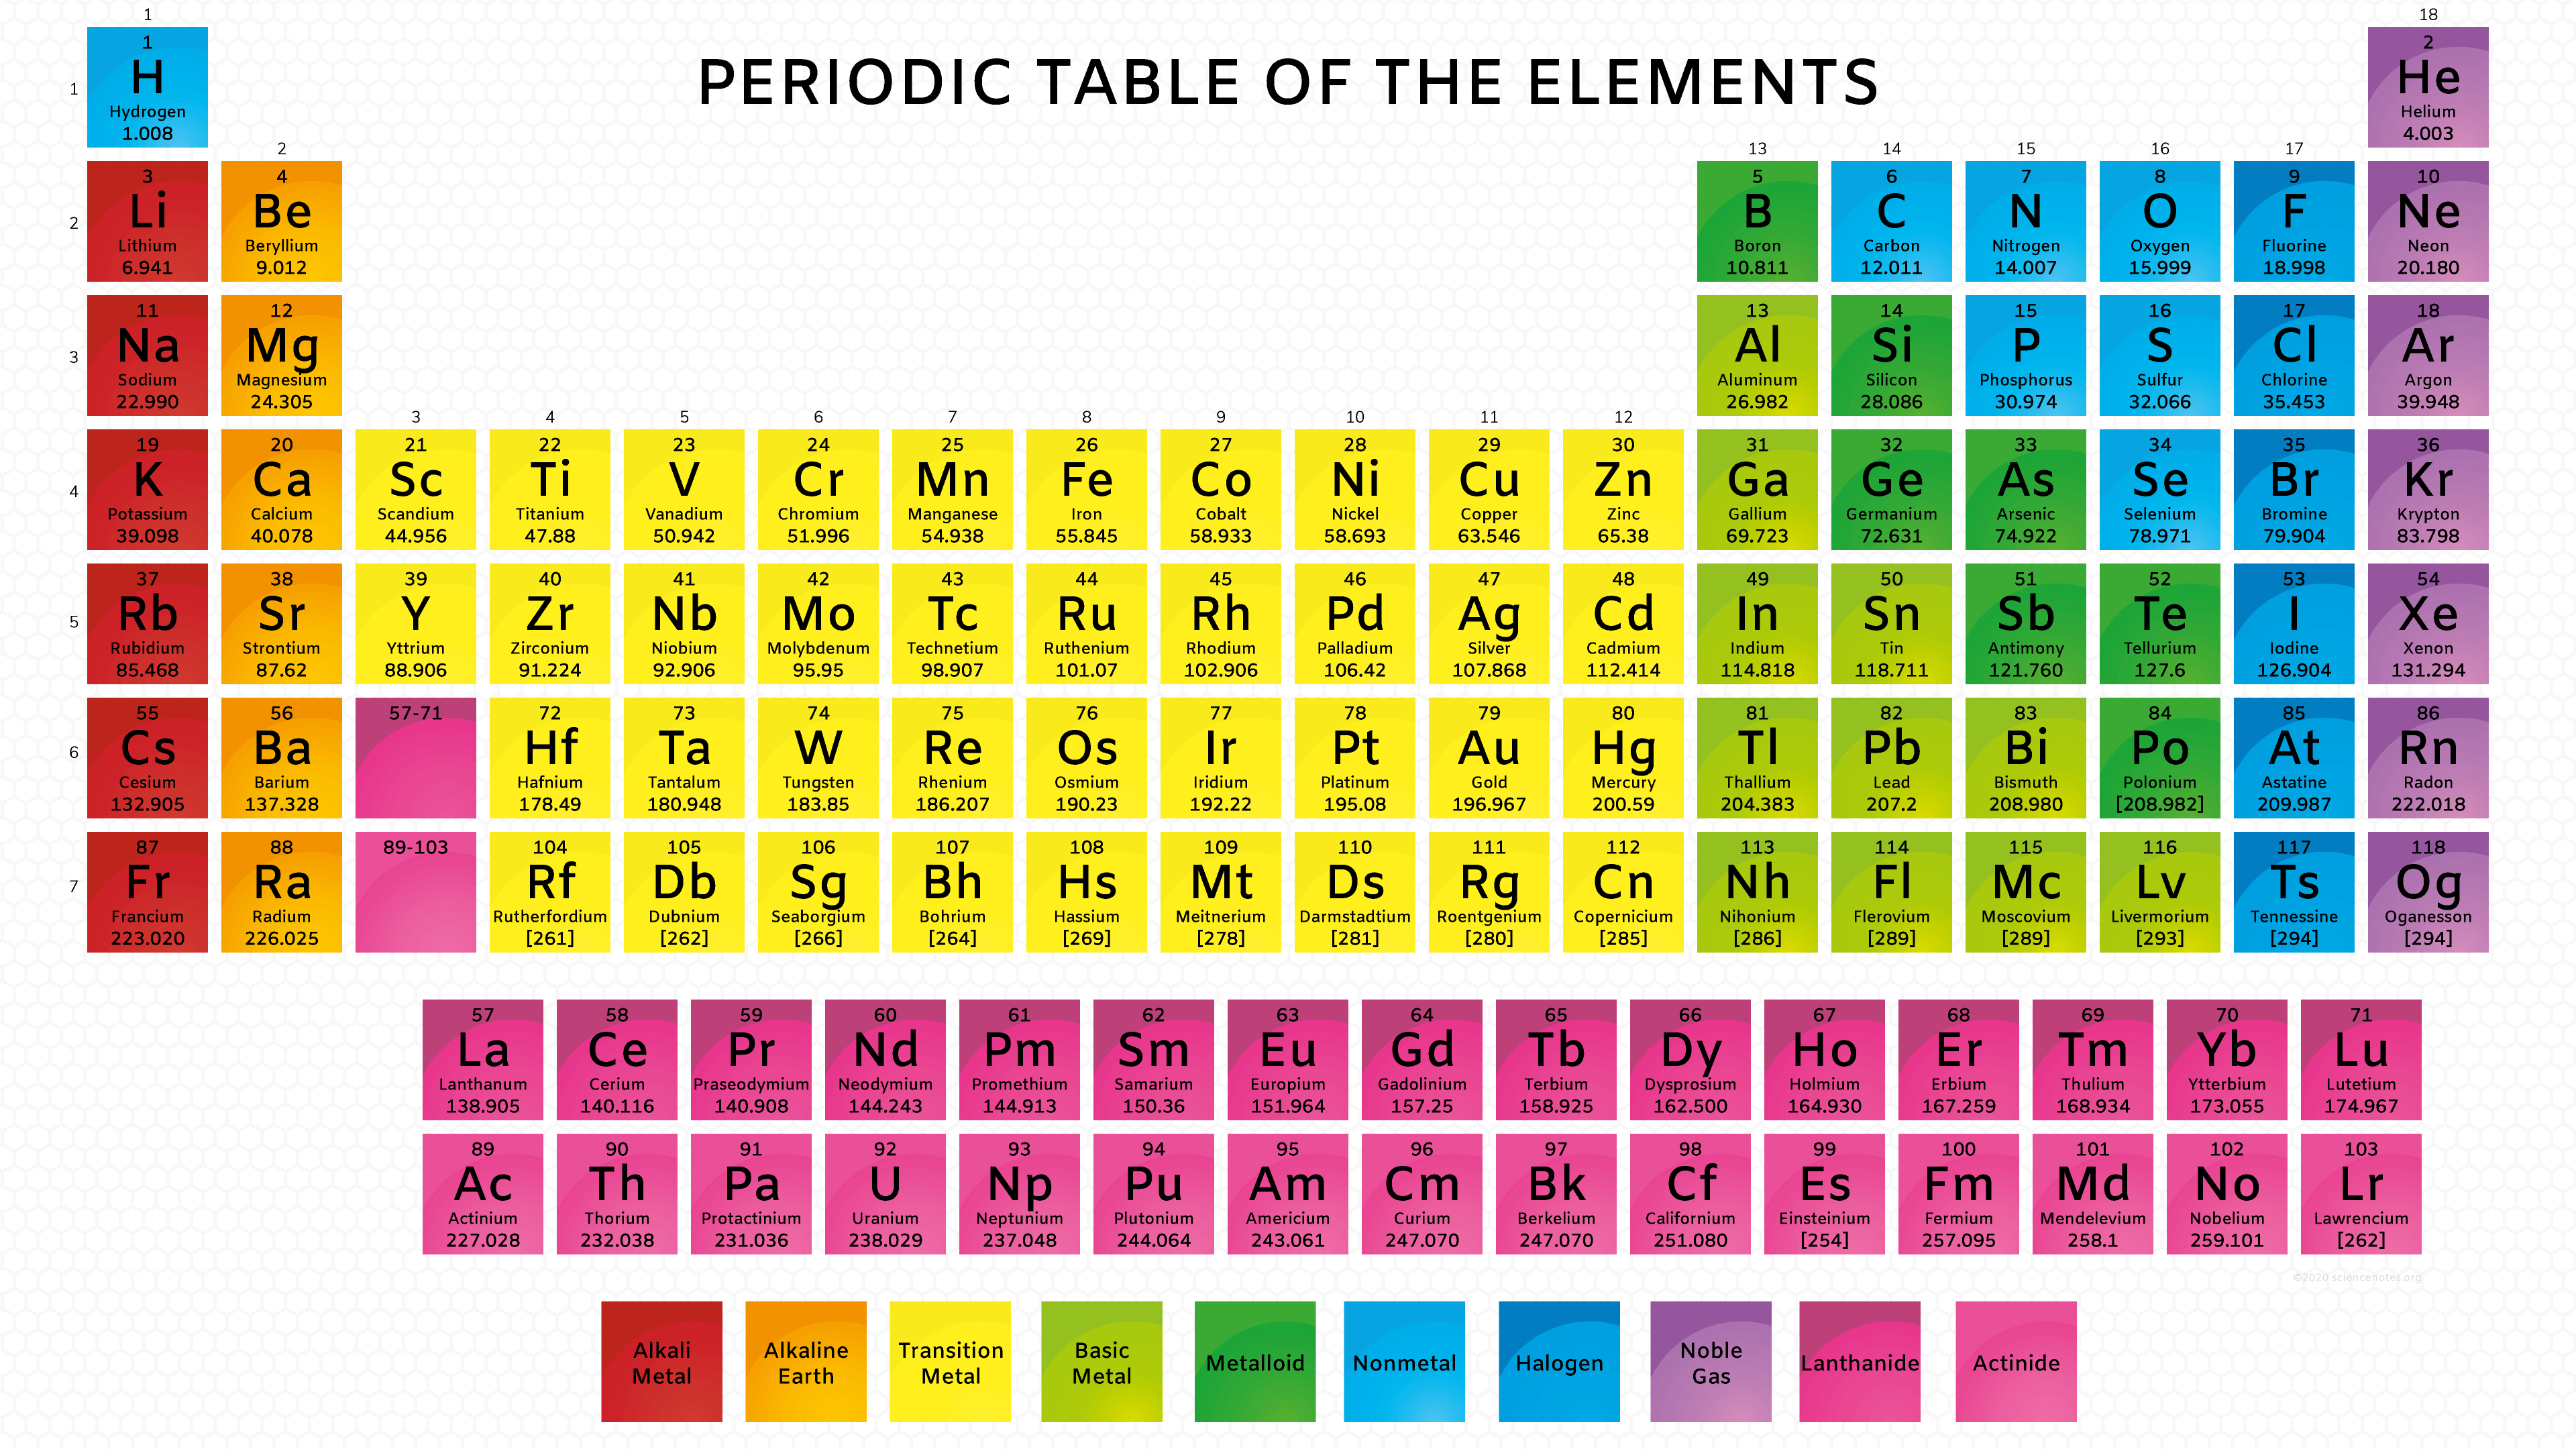
\includegraphics[trim={0cm 0cm 0cm 0cm},clip, keepaspectratio,width=0.99\textwidth]{PeriodicTableAtomicMassColor}\label{fig:PeriodicTableAtomicMassColor}
\end{figure}
\end{frame}

\begin{frame}{Energy prodcution PP chains ($\SI{1}{\mega\ev}=\SI{1.602e-6}{\erg}$)}
    \begin{columns}[T]
        \begin{column}{0.45\textwidth}
\begin{figure}[!ht]
    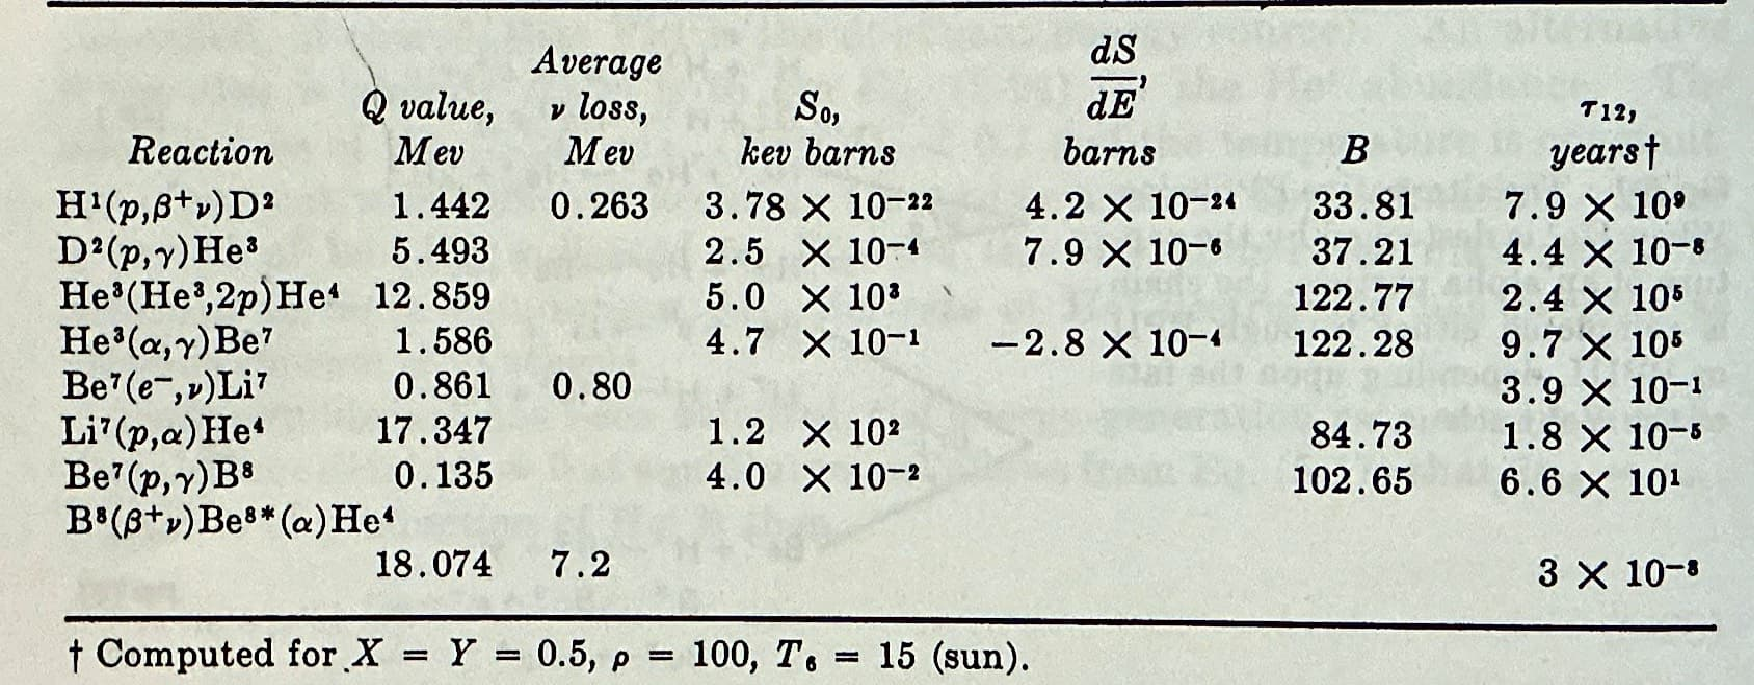
\includegraphics[trim={0cm 0cm 0cm 0cm},clip, keepaspectratio,width=0.99\textwidth]{pp-Q-table}\label{fig:pp-Q-table}
\end{figure}
    \begin{itemize}
        \item PPII, PPIII - $He^3(He^4,\gamma)Be^7$ then electron capture $Be^7+\Pelectron\to Li^7+\nu$ (or proton captur: $Be^7+H^1\to B^8+\gamma$): rate of prodiuction of $\alpha$ may be up to twice that of PPI ($\frac{r_{pp}}{2}$) as only one PP reaction. Approx:
            \begin{itemize}
                \item Deuterium equilibrium(seconds-hours): $\TDy{t}{D}\approx0$ quindi $\lambda_{pp}\frac{H^2}{2}\approx\lambda_{pd}HD$
        \item $Li^7$, $Be^7$ equilibrium: $\TDy{t}{Li^7+Be^7}=\lambda_{34}He^3He^4-\lambda_{17}HBe^7-\lambda_{17}'HLi^7\approx0$, when equilibrium reached (years) Li/Be will follow buildup of $He^3$ - simplified equation for rate of production of $He^4$ and H: 
            \begin{align*}
                &\TDy{t}{He^4}=\lambda_{33}\frac{(He^3)^2}{2}+\lambda_{34}He^3He^4\\
                &\TDy{t}{H}=-3\lambda_{pp}\frac{H^2}{2}+2\lambda_{33}\frac{(He^3)^2}{2}-\lambda_{34}He^3He^4
            \end{align*}
            Competition for $He^3$ determines which PP dominates
            \end{itemize}
    \end{itemize}
        \end{column}
        \begin{column}{0.55\textwidth}
        PPI - Split in two parts: pp is followed rapidly by $D(p,\gamma)He^3$ (net effect $3H\to He^3+\nu$) at rate $r_{pp}$, energy liberated $Q=\SI{6.936}{\mega\ev}-\SI{0.263}{\mega\ev}$ so $\rho\epsilon(3H\to He^3)=\num{1.069e-5}r_{pp}\si{\erg\per\cubic\cm\per\second}$ - then for $He^3(He^3,2p)He^4$ has $Q=\SI{12.858}{\mega\ev}$ and summing $\rho\epsilon_{PPI}=\num{1.069e-5}r_{pp}+\num{2.060e-5}r_{33}\si{\erg\per\cubic\cm\per\second}$. Equilibrium $\TDy{t}{He^3}\approx0$: $2r_{33}=r_{pp}$, $\TDy{t}{He^4}=r_{33}=\frac{r_{pp}}{2}$ and energy production $\rho\epsilon_{PPI}=\num{2.099e-5}r_{pp}\si{\erg\per\cubic\cm\per\second}$.
        \begin{itemize}
            \item Third approx when $He^3$ reaches equilibrium:
                \begin{align*}
                    &\TDy{t}{He^3}\approx0\Rightarrow\lambda_{pp}-\lambda_{33}(He^3_e)^2-\lambda_{34}He_e^3He^4\approx0\\
                    &\TDy{t}{He^4}=\frac{1}{4}\lambda_{pp}H^2+\frac{1}{2}\lambda_{34}He_e^3He^4\\
                    &\TDy{t}{H}=-\lambda_{pp}^2-2\lambda_{34}He_e^3He^4\\
                    &\TDy{t}{He^4}=-\frac{1}{4}\TDy{t}{H}\tag{All reactions in equil.}\\
                    &\left(\frac{PP1}{PPII+PPIII}\right)_e=\frac{1}{2}\frac{\lambda_{33}}{\lambda_{34}}\frac{He_e^3}{He^4}\\
                    &PPI: \frac{2*0.263}{26.73}\approx2.0\%\ PPII: \frac{0.263+0.80}{26.73}\approx4.0\%\\
                    &PPIII: \frac{0.263+7.2}{26.73}\approx27.9\%\tag{$\nu$ losses}
                \end{align*}
        \end{itemize}
        \end{column}
    \end{columns}
\end{frame}

\begin{frame}{Approfondimenti PP}
    \begin{columns}[T]
        \begin{column}{0.4\textwidth}
            \begin{figure}[!ht]
    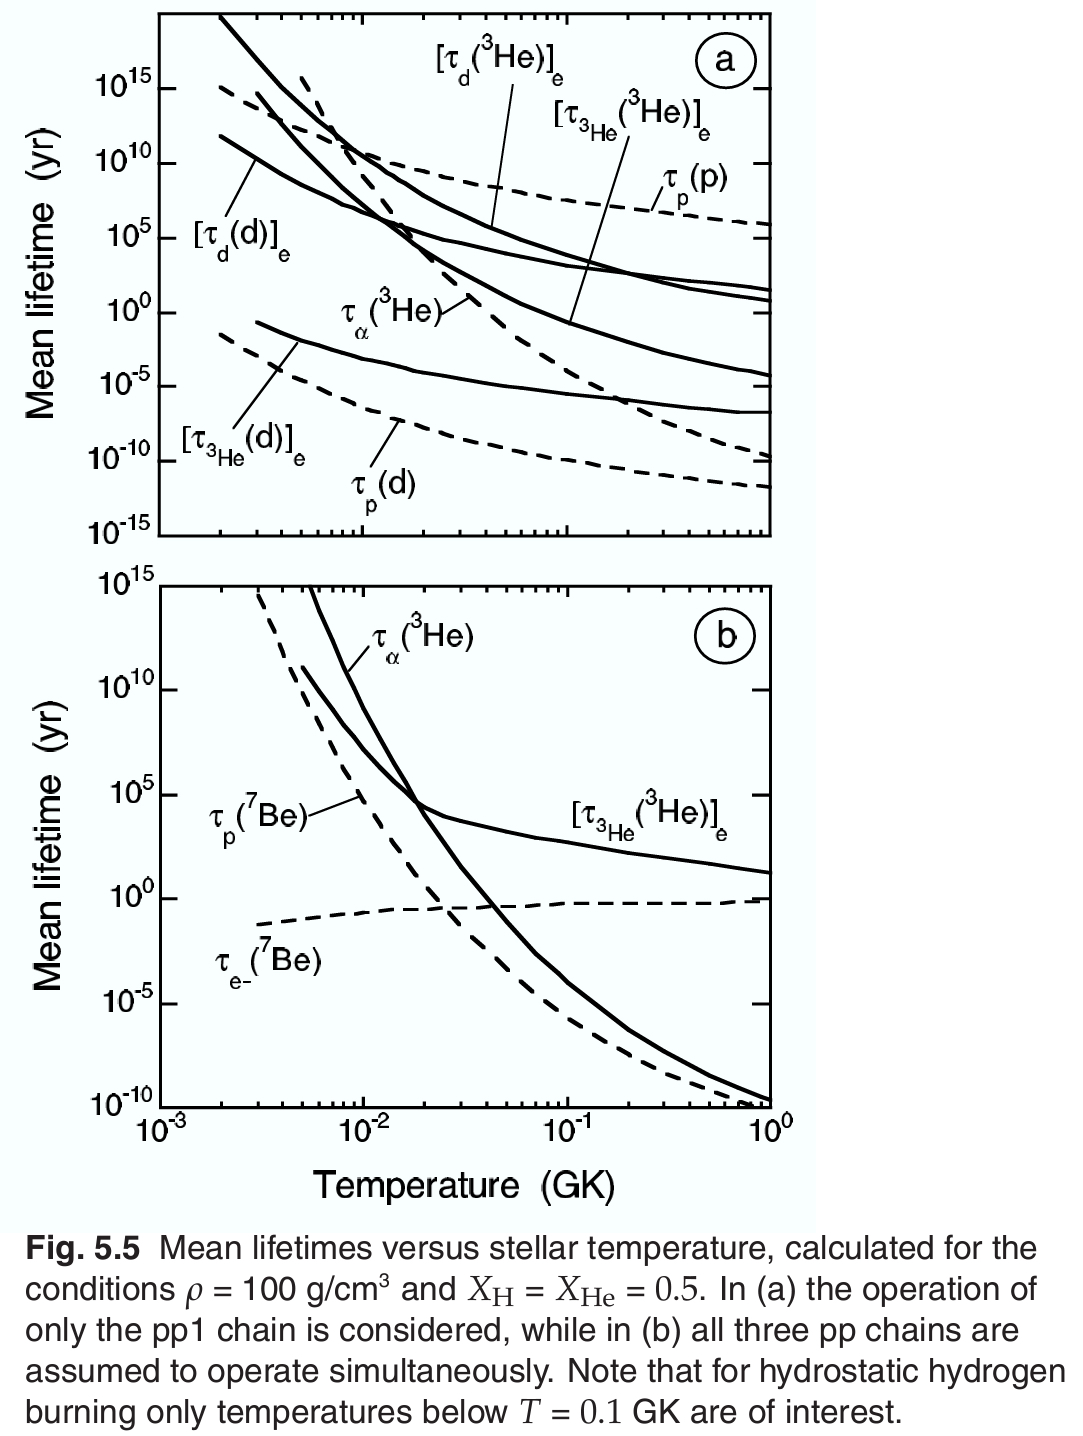
\includegraphics[trim={0cm 0cm 0cm 0cm},clip, keepaspectratio,height=0.9\textheight]{PP-lifetime}\label{fig:PP-lifetime}
\end{figure}
        \end{column}
        \begin{column}{0.6\textwidth}
            \begin{align*}
                &Q=(4(ME)_{H}-(ME)_{He^4})c^2=\SI{26.731}{\mega\ev}\\
                &\rho\epsilon=\TDy{t}{He^4}(4M_H-M_{He^4})[0.980F_{PPI}+0.960F_{PPII}+0.721F_{PPIII}]\\
                &\rho\epsilon_{PPI}=\SI{6.671}{\mega\ev}r_{pp}+\SI{12.861}{\mega\ev}r_{He^3He^3}\\
                &\epsilon_{pp}^e=\num{6.551}N_A\exv{\sigma v}_{pp}(\frac{X_H}{M_H}^2\rho N_A\si{\mega\ev\per\gram\per\second}\\
                    &\epsilon_{PPI}^e=\epsilon_{PPI}^e(T_0)(\frac{T}{T_0})^{3.9}
            \end{align*}
            \begin{figure}[!ht]
    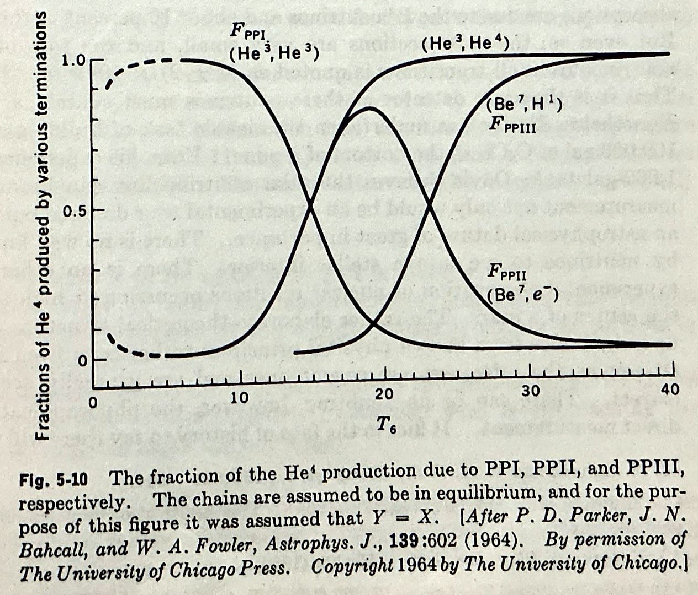
\includegraphics[trim={0cm 0cm 0cm 0cm},clip, keepaspectratio,width=0.75\textwidth]{PP-energy-fraction}\label{fig:PP-energy-fraction}
\end{figure}
        \end{column}
    \end{columns}
\end{frame}

\begin{frame}{Ciclo CN-NO}
    \begin{columns}[T]
        \begin{column}{0.4\textwidth}
\begin{figure}[!ht]
    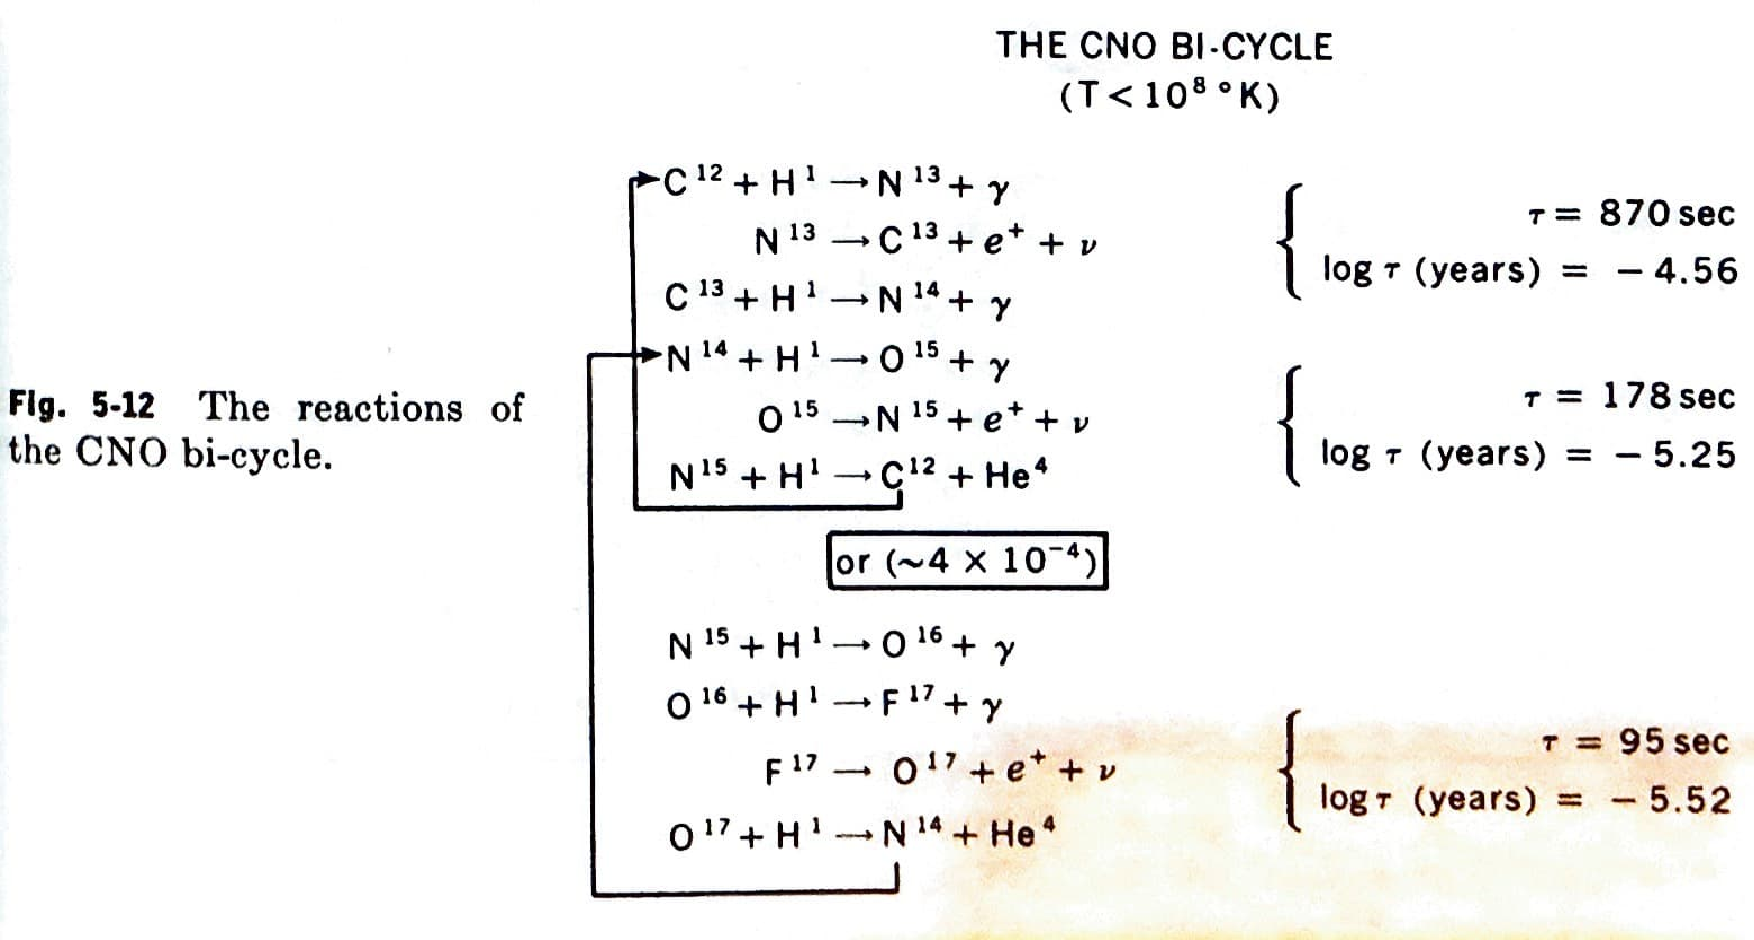
\includegraphics[trim={0cm 0cm 0cm 0cm},clip, keepaspectratio,width=0.99\textwidth]{cnno-scheme}\label{fig:cnno-scheme}
    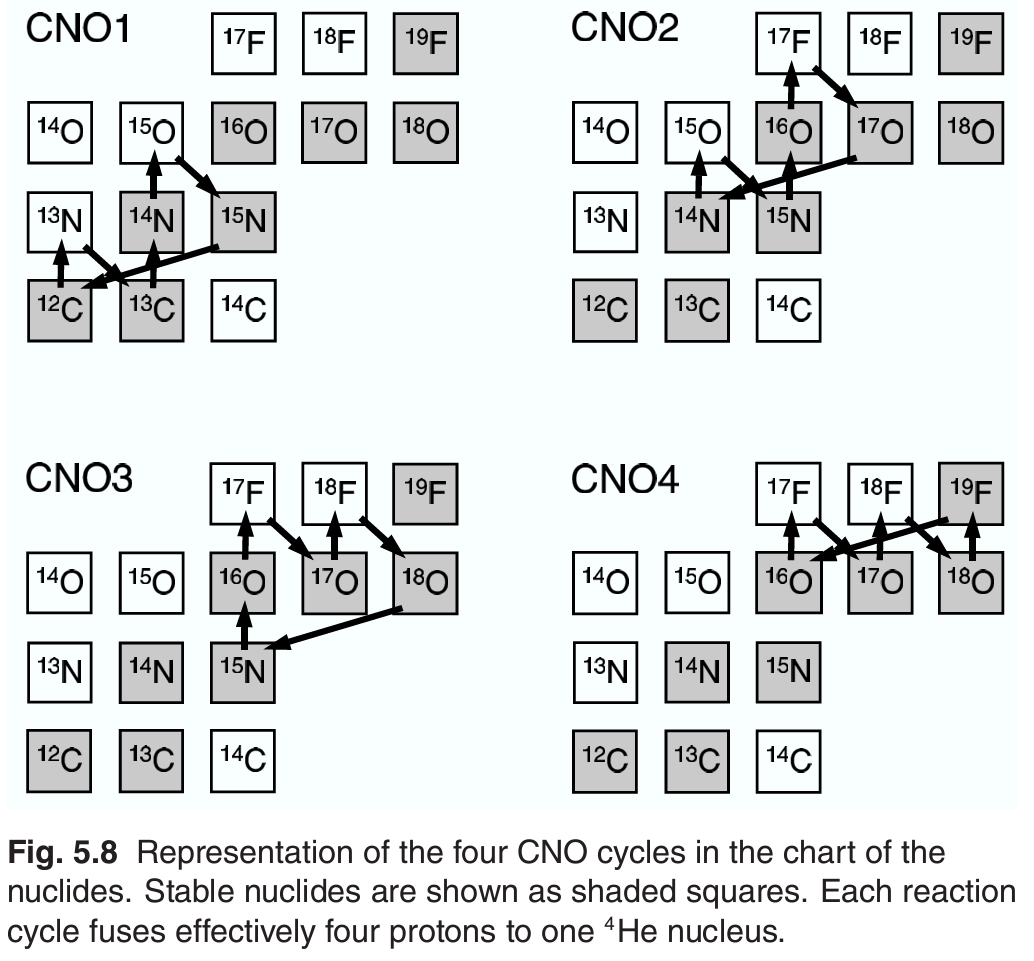
\includegraphics[trim={0cm 0cm 0cm 0cm},clip, keepaspectratio,width=0.99\textwidth]{CNOs}\label{fig:cnos}
\end{figure}
        \end{column}
        \begin{column}{0.6\textwidth}
            Energetic. allowed: proton induced $(p,\alpha)$ reactions on $^{15}N$, $^{17}O$, $^{18}O$, $(p,\gamma)$ and $(p,\alpha)$ on $^{19}F$, and only $(p,\gamma)$ on $^{12}C$, $^{13}C$, $^{14}N$, $^{16}O$.
            \begin{align*}
                &C^{12}(p,\gamma)N^{13}(\beta^+\nu)C^{13}(p\gamma)N^{14}\tag{CN-CNO1}\\
                &N^{14}(p,\gamma)O^{15}(\beta^+\nu)N^{15}\\
                &N^{15}(p,\alpha)C^{12}\\
                &N^{15}(p,\gamma)O^{16}(p,\gamma)F^{17}(\beta^+\nu)O^{17}\tag{NO-CNO2}\\
                &O^{17}(p,\alpha)N^{14}\\
                &O^{17}(p,\gamma)F^{18}(\beta^+\nu)O^{18}(p,\alpha)N^{15}\tag{CNO3}\\
                &O^{18}(p,\gamma)F^{19}(p,\alpha)O^{16}\tag{CNO4}
            \end{align*}
\begin{figure}[!ht]
    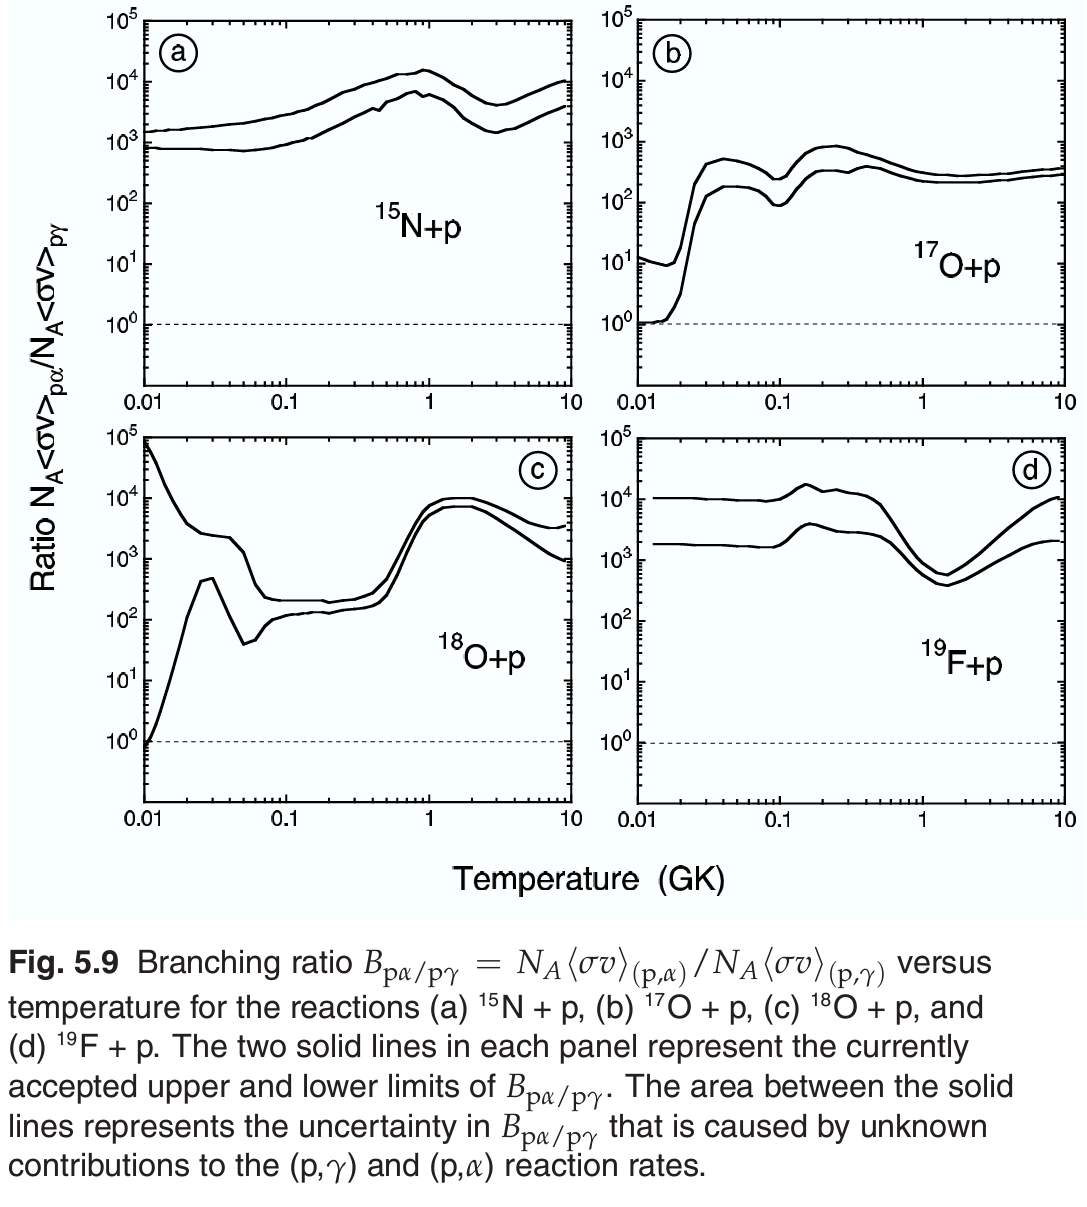
\includegraphics[trim={0cm 0cm 0cm 0cm},clip, keepaspectratio,width=0.65\textwidth]{CNObranching}\label{fig:CNObranching}
\end{figure}
        \end{column}
    \end{columns}
\end{frame}

\begin{frame}{Steady state CNO: Abundances}
    \begin{columns}[T]
        \begin{column}{0.5\textwidth}
            For $T<\SI{0.1}{\giga\ev}$ $\beta$-decay lifetime of $^{13}N$ $\tau_{^{13}N}\ll\tau_{^{12}C}$ for $(p,\gamma)$ destruction, and after few minutes $^{13}N$, $^{15}O$ are at equilibrium
            \begin{align*}
                &\TDy{t}{^{12}C}=H ^{15}N\exv{\sigma v}_{^{15}N(p,\alpha)}-H ^{12}C\exv{\sigma v}_{^{12}C(p,\gamma)}\\
                &\TDy{t}{^{13}C}=H ^{12}C\exv{\sigma v}_{^{12}C(p,\gamma)}-H ^{13}C\exv{\sigma v}_{^{13}C(p,\gamma)}\\
                &\TDy{t}{^{14}N}=H ^{13}C\exv{\sigma v}_{^{13}C(p,\gamma)}-H ^{14}N\exv{\sigma v}_{^{14}N(p,\gamma)}\\
                &\TDy{t}{^{15}N}=H ^{14}N\exv{\sigma v}_{^{14}N(p,\alpha)}-H ^{15}N\exv{\sigma v}_{^{15}N(p,\alpha)}\\
                &\left(\frac{^{14}N}{^{12}C}\right)_e=\frac{\exv{\sigma v}_{^{12}C(p,\gamma)}}{\exv{\sigma v}_{^{14}N(p,\gamma)}}=\frac{\tau_p(^{14}N)}{\tau_p(^{12}C)}
            \end{align*}
        \end{column}
        \begin{column}{0.5\textwidth}
            \begin{align*}
                &\Rightarrow\TDy{t}{^{12}C}+\TDy{t}{^{13}C}+\TDy{t}{^{14}N}+\TDy{t}{^{15}N}=0\\
                &\Rightarrow\sum CNO1=\const{}
            \end{align*}
            Ratio of any nuclidic abb. is inverse ratio of reaction rate (or lifetime): ie $(\frac{^{14}N}{^{12}C})=\frac{\exv{\sigma v}_{^{12}C(p,\gamma)}}{\exv{\sigma v}_{^{14}N(p,\gamma)}}$. CNO abundance evolution: conversion of $^{12}C$, $^{16}O$ to $^{14}N$.
        \end{column}
    \end{columns}
    \begin{figure}[!ht]
    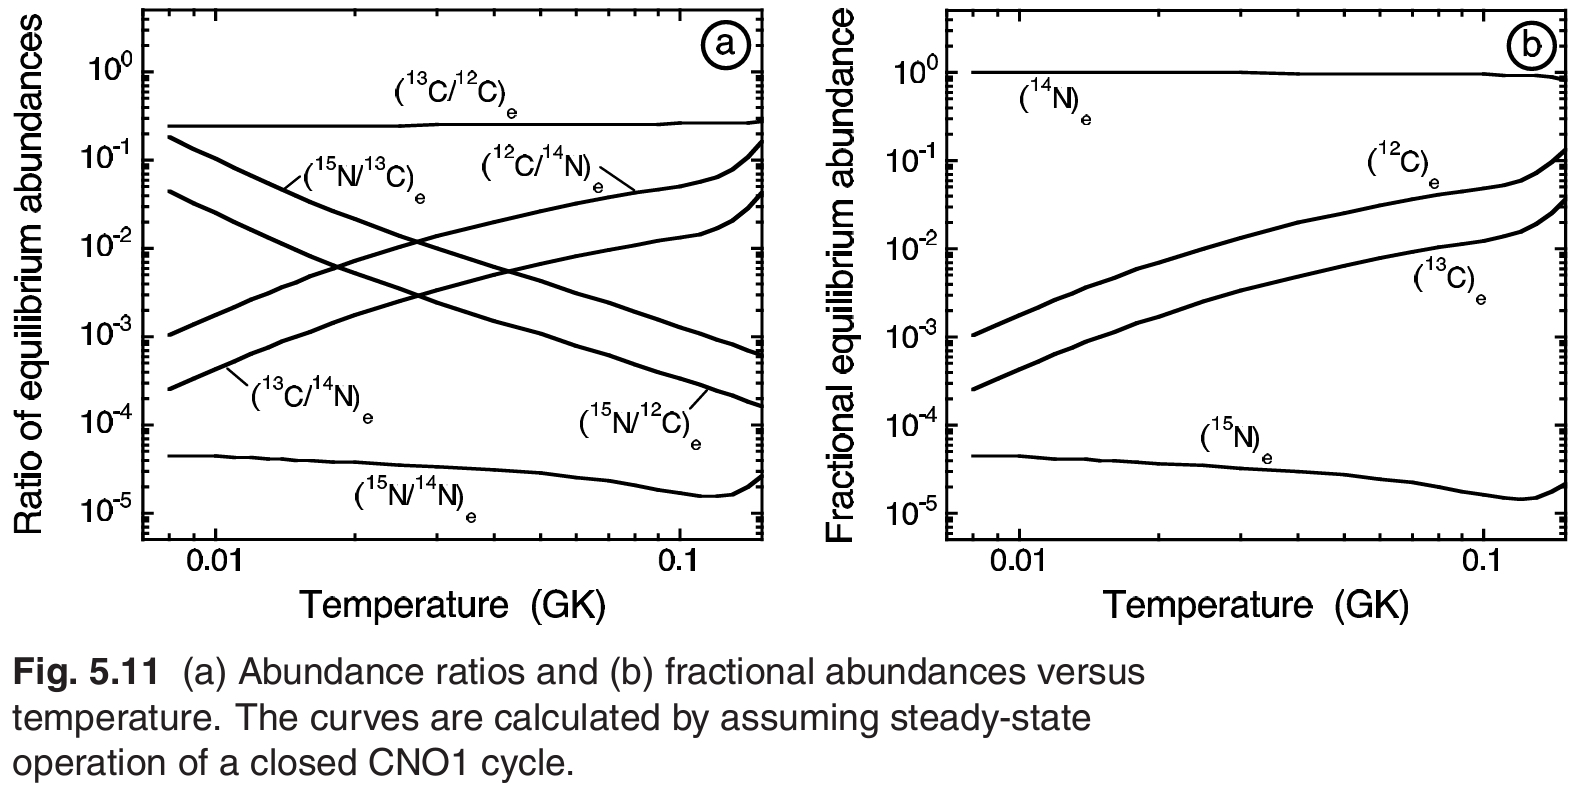
\includegraphics[trim={0cm 0cm 0cm 0cm},clip, keepaspectratio,width=0.65\textwidth]{CNO1-equil-abund}\label{fig:CNO1-equil-abund}
\end{figure}
\end{frame}

\begin{frame}{Steady state CNO: energy production}
            \begin{align*}
                &\epsilon_{CNO}=\frac{1}{\rho}\sum_{i\to j}(Q_{i\to j}-\bar{E}^{i\to j}_{\nu})r_{i\to j}\\
                &Q_{^{12}C(p,\gamma)^{13}N(\beta^+\nu)}-\bar{E}^{^{13}N(\beta^+\nu)}=(\num{1.944}+\num{2.22}-\num{0.706})\si{\mega\ev}=\SI{3.458}{\mega\ev}\\
                &Q_{^{13}C(p,\gamma)}=\SI{7.551}{\mega\ev}\\
                &Q_{^{14}N(p,\gamma)^{15}O(\beta^+\nu)}-\bar{E}_{\nu}^{^{15}(\beta^+\nu)}=(\num{7.297}+\num{2.754}-\num{0.996})\si{\mega\ev}=\SI{9.055}{\mega\ev}\\
                &Q_{^{15}N(p,\alpha)}=\SI{4.966}{\mega\ev}\\
                &\rho\epsilon^e_{CNO1}=\SI{3.458}{\mega\ev}H(^{12}C)_e\exv{\sigma v}_{^{12}C(p,\gamma)}+\SI{7.551}{\mega\ev}H(^{13}C)_e\exv{\sigma v}_{^{13}C(p,\gamma)}+\SI{9.055}{\mega\ev}H(^{14}N)_e\exv{\sigma v}_{^{14}N(p,\gamma)}\\
                &+\SI{4.966}{\mega\ev}H(^{15}N)_e\exv{\sigma v}_{^{15}N(p,\alpha)}\\
                &=\SI{3.458}{\mega\ev}\frac{(^{12}C)_e}{\tau_p(^{12}C)}+\SI{7.551}{\mega\ev}\frac{(^{13}C)_e}{\tau_p(^{13}C)}+\SI{9.055}{\mega\ev}\frac{(^{14}N)_e}{\tau_p(^{14}N)}+\SI{4.966}{\mega\ev}\frac{(^{15}N)_e}{\tau_p(^{15}N)}\\
                &\epsilon^e_{CNO1}=\frac{\SI{25.030}{\mega\ev}}{\rho}\frac{\sum CNO1}{\tau_p(^{12}C)+\tau_p(^{13}C)+\tau_p(^{14}N)+\tau_p(^{15}N)}\approx\frac{\SI{25.030}{\mega\ev}}{\rho}\frac{\sum CNO1}{\tau_p(^{14}N)}\\
                &=\frac{\SI{25.030}{\mega\ev}}{\rho}(\sum CNO1)H\exv{\sigma v}_{^{14}N(p,\gamma)}=\num{25.030}N_A\exv{\sigma v}_{^{14}N(p,\gamma)}(\sum_i \frac{X_i}{M_i})\frac{X_H}{M_H}\rho N_A\si{\mega\ev\per\gram\per\second}\\
                &\epsilon^e_{CNO1}(T)=\epsilon^e_{CNO1}(T_0)(\frac{T}{T_0})^{16.7}\tag{$T=\SI{25}{\mega\kelvin}$}\\
                &\epsilon_{pp}\propto\rho X_H^2,\ \epsilon_{CN}\propto\rho X_HX_{CN}
            \end{align*}
\end{frame}

\begin{frame}{He burning: energy production}
    He-burn in massive* contribute $^{16}O$, $^{18}O$ to universe while massive* and AGB of $^{12}C$.
    \begin{columns}[T]
        \begin{column}{0.7\textwidth}
            \begin{align*}
                &^4He(\alpha\alpha,\gamma)^{12}C\tag{$Q=\SI{7274.7}{\kilo\ev}$}\\
                &\alpha+\alpha\to^8Be\tag{$Q=\SI{-91.84\pm0.04}{\kilo\ev}$}\\
                &E_r=\SI{287.6\pm0.2}{\kilo\ev}\tag{Res in $^8Be(\alpha,\gamma)^{12}C$}\\
                &^{12}(\alpha,\gamma)^{16}O\tag{$Q=\SI{7161.9}{\kilo\ev}$}\\
                &^{16}O(\alpha,\gamma)^{20}Ne\tag{$Q=\SI{4729.8}{\kilo\ev}$}\\
                &^{20}Ne(\alpha,\gamma)^{24}Mg\tag{$Q=\SI{9316.6}{\kilo\ev}$}\\
                &\lambda_{3\alpha\to^{12}C}=\lambda_{3\alpha}=3N_{\alpha}(\frac{h^2}{2\pi})^{\frac{3}{2}}\frac{1}{(m_{\alpha\alpha}KT)^{\frac{3}{2}}}\exp{\frac{Q_{\alpha\alpha\to^8Be}}{KT}}\lambda_{^8Be(\alpha,\gamma)}\\
                &\lambda_{^8Be(\alpha,\gamma)}=\lambda_{\alpha}(^8Be)=N_{\alpha}\exv{\sigma v}_{^8Be(\alpha,\gamma)}\\
                &\sigma_{^8Be(\alpha,\gamma)}=(\frac{2\pi}{m_{\alpha^8Be}KT})^{\frac{3}{2}}\hbar^2\exp{\frac{E_r}{KT}}\omega\gamma_{^8Be(\alpha,\gamma)}\tag{Narrow res.}\\
                &\omega\gamma_{^8Be(\alpha,\gamma)}=\frac{2J+1}{(2j_0+1)(2j_1+1)}\frac{\Gamma_{\alpha}\Gamma_{rad}}{\Gamma}\approx\Gamma_{rad}\approx\SI{3.7\pm0.5}{\milli\ev}\\
                &\Gamma_{\alpha}=\SI{8.3\pm0.1}{\ev},\ \Gamma_{rad}=\Gamma_{\gamma}+\Gamma_{pair}=\SI{3.7\pm0.5}{\milli\ev},\\
                &J(^{12}C)=j_0(\alpha)=j_1(^8Be)=0\\
                &\lambda_{3\alpha}=\num{8.7590e-10}\frac{(\rho X_{\alpha})^2}{T_9^3}\exp{\frac{-\num{4.4040}}{T_9}}\si{\per\second}\tag{$E'=\SI{287.6}{\kilo\ev}-\SI{-91.84}{\kilo\ev}=\SI{379.4}{\kilo\ev}$}\\
                &\epsilon_{3\alpha}=\frac{Q_{3\alpha}}{\rho}r_{3\alpha}=\frac{\SI{7.275}{\mega\ev}}{\rho}\frac{1}{3}\num{8.7590e-10}(\rho N_A \frac{X_{\alpha}}{M_{\alpha}})\frac{(\rho X_{\alpha})}{T_9^3}\exp{-\frac{\num{4.4040}}{T_9}}\\
                &=\num{3.1771e14}\frac{\rho^2X_{\alpha}^3}{T_9^3}\exp{-\frac{4.4040}{T_9}}\si{\mega\ev\per\gram\per\second}
            \end{align*}
        \end{column}
        \begin{column}{0.3\textwidth}
            $\rho=\SIrange{e2}{e5}{\gram\per\cubic\cm}$, $T=\SIrange{0.1}{0.4}{\giga\kelvin}$
\begin{figure}[!ht]
    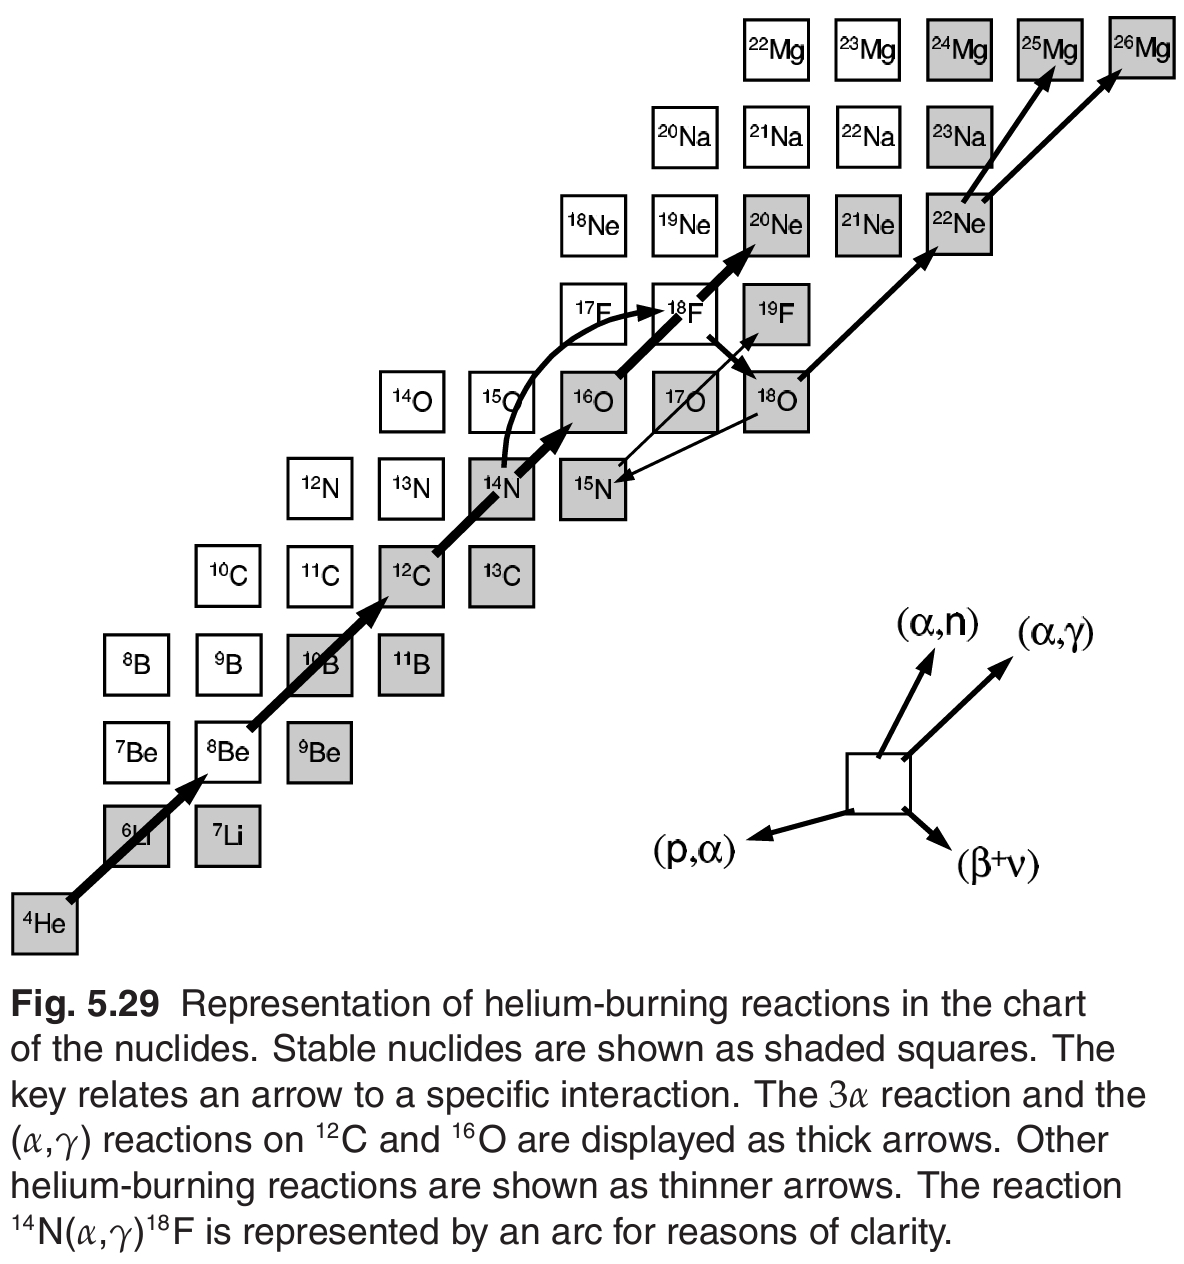
\includegraphics[trim={0cm 0cm 0cm 0cm},clip, keepaspectratio,height=0.40\textheight]{Heburning-network}\label{fig:Heburning-network}
\end{figure}
    \begin{align*}
        &\epsilon_{3\alpha}(T)=\epsilon_{3\alpha}(T_0)(\frac{T}{T_0})^{41.0}\\
        &\frac{N(^{12}C)}{N(^{16}O)}\tag{universe}
    \end{align*}
    \todo{Iliadis: He burning beyonf C}
        \end{column}
    \end{columns}
\end{frame}

\begin{frame}{Advanced Burning Stages ($T>\SI{6e8}{\kelvin}$): C-Burning}
    \begin{columns}[T]
        \begin{column}{0.45\textwidth}
            Coulomb barrier $CC$: \SI{8}{\mega\ev}
            \begin{align*}
                &C^{12}+C^{12}&\to Mg^{24}+\gamma\tag{$Q=\SI{13.930}{\mega\ev}$}\\
                &&\to Na^{23}+p\tag{$Q=\SI{2.238}{\mega\ev}$}\\
                &&\to Ne^{20}+\alpha\tag{$Q=\SI{4.616}{\mega\ev}$}\\
                &&\to Mg^{23}+n\tag{\xaumenta{T}:shell $Q=\SI{-2.6}{\mega\ev}$}\\
                &&\to O^{16}+2\alpha\tag{$Q=\SI{-0.11}{\mega\ev}$}\\
                &O^{16}+O^{16}&\to S^{32}+\gamma\tag{$Q=\SI{16.539}{\mega\ev}$}\\
                &&\to P^{31}+p\tag{$Q=\SI{7.676}{\mega\ev}$}\\
                &&\to S^{31}+n\tag{$Q=\SI{1.459}{\mega\ev}$}\\
                &&\to Si^{28}+\alpha\tag{$Q=\SI{9.593}{\mega\ev}$}\\
                &&\to Mg^{24}+2\alpha\tag{$Q=\SI{-0.4}{\mega\ev}$}
            \end{align*}
\begin{figure}[!ht]
    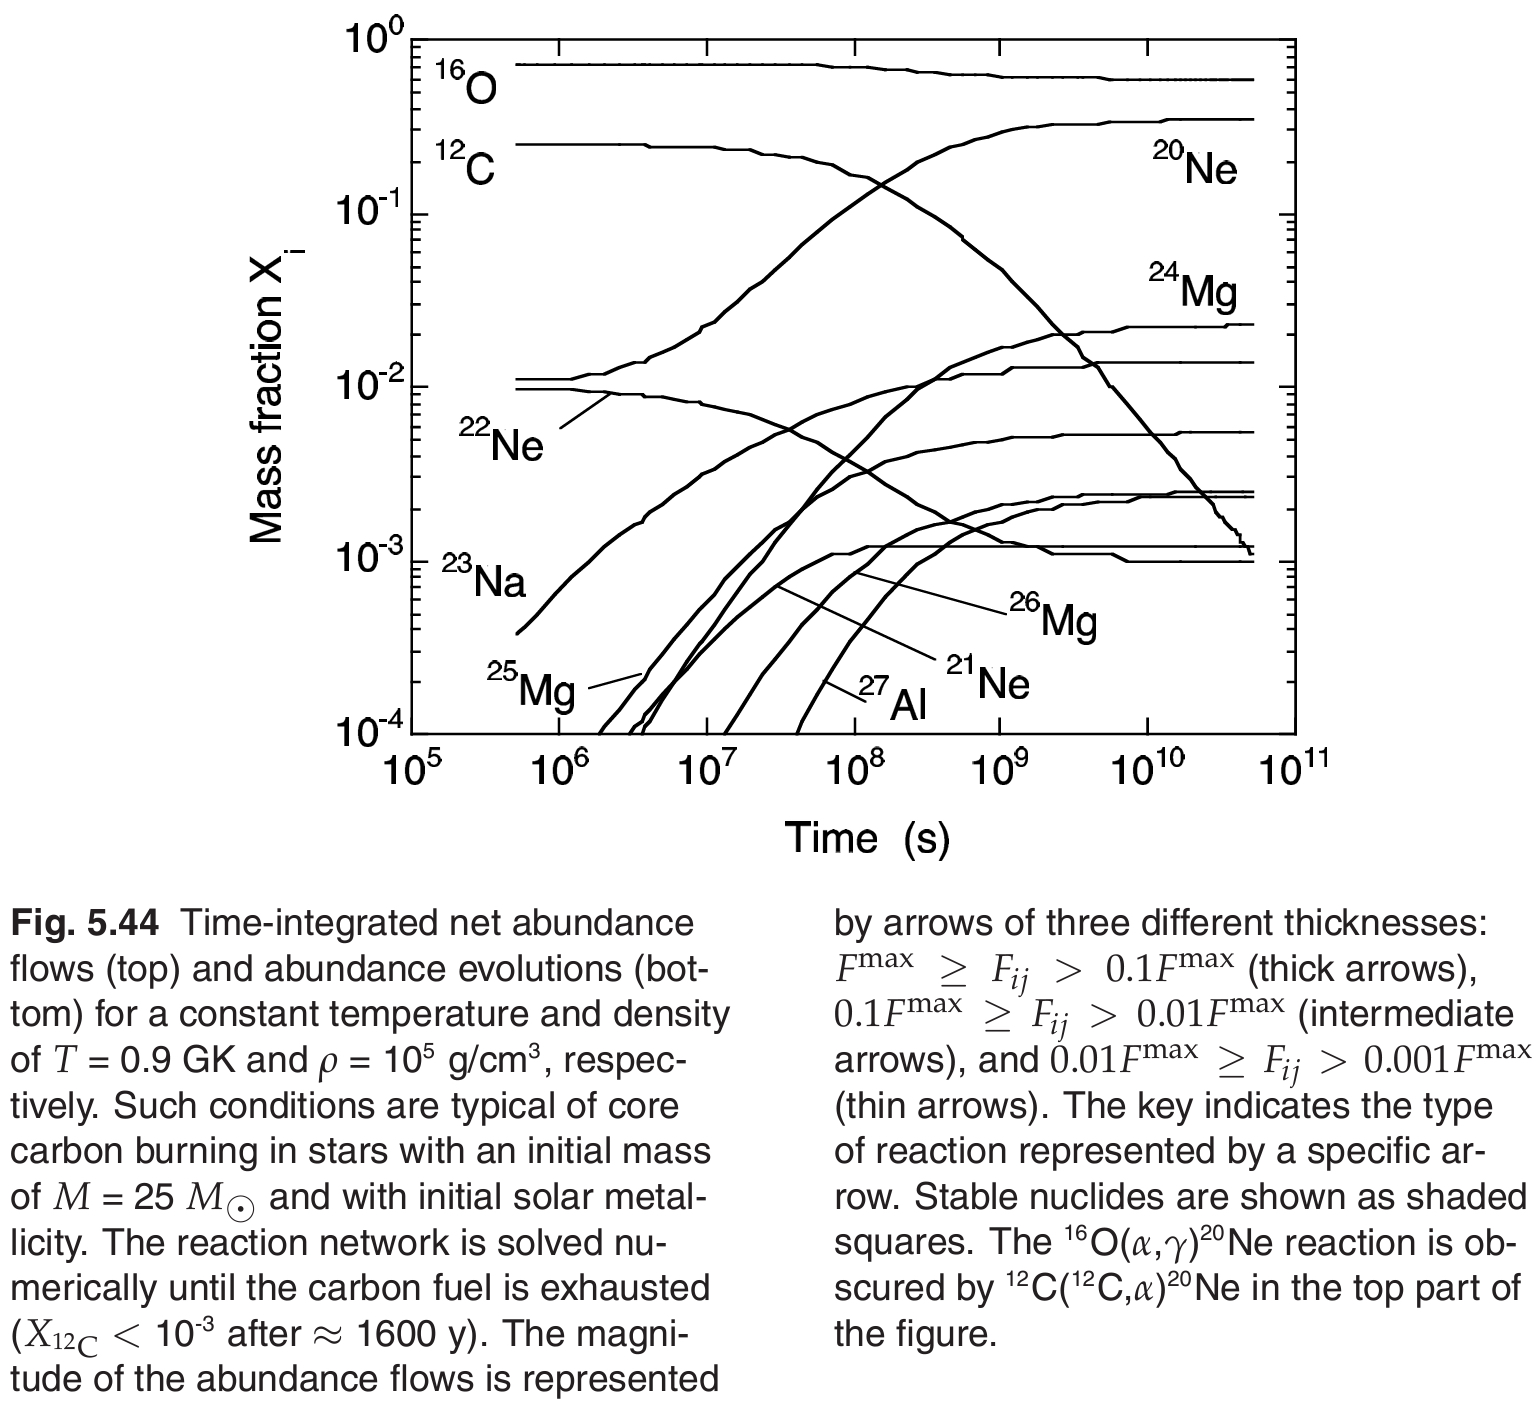
\includegraphics[trim={0cm 0cm 0cm 0cm},clip, keepaspectratio,height=0.32\textheight]{CBurning-abund}\label{fig:CBurning-abund}
\end{figure}
        \end{column}
        \begin{column}{0.55\textwidth}
            Difference mass between compound nucleus $^{12}C+^{12}C$ and $^{24}Mg$: excess energy carried away from light massive particles (Branching ratio $B_p\approx B_{\alpha}\approx \frac{1-B_n}{2}$, $B_n\approx2-10\%$ at $E_{cm}=\SIrange{3.5}{5.0}{\mega\ev}$): $^{12C(^{12}C,\alpha)}$ and $^{12}(^{12}C,p)$ rates approx equal while $^{12}C(^{12}C,n)$ is far smaller. Important electron screening correction: approx factor 3. Secondary reactions contribute sign. to nuclear energy release by primary C-burning: each $^{12}C+^{12}C$ releases $\bar{Q}_C\approx\SI{10}{\mega\ev}$
            \begin{align*}
                &\epsilon_C=\frac{\bar{Q}_C}{\rho}r_{^{12}C^{12}C}=\frac{\bar{Q}_C}{\rho}\frac{(N_{^{12}C})^2\exv{\sigma v}_{^{12}^{12}C}}{2}\\
                &=\frac{N_A\bar{Q}_C}{288}X_{^{12}C}^2\rho N_A\exv{\sigma v}_{^{12}C^{12}C}=\num{2.09e22}X_{^{12}C}^2\rho N_A\exv{\sigma v}_{^{12}C^{12}C}\\
            \end{align*}
\begin{figure}[!ht]
    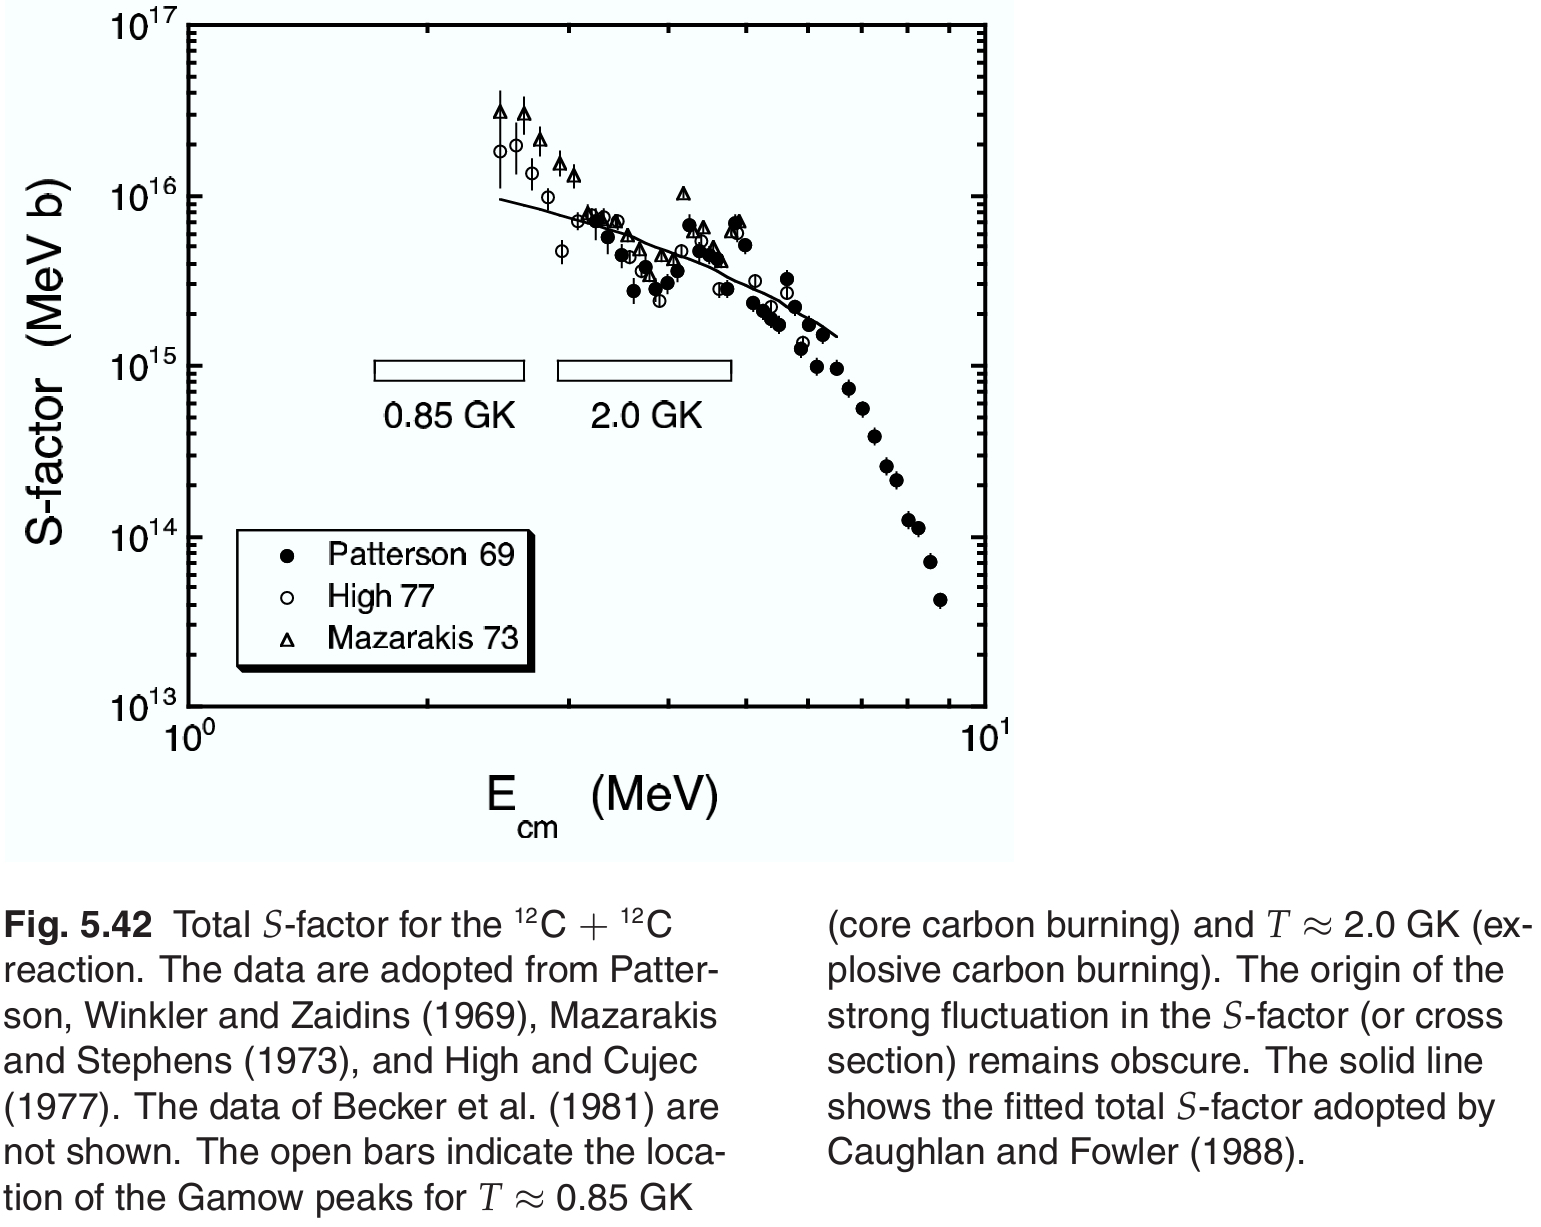
\includegraphics[trim={0cm 0cm 0cm 0cm},clip, keepaspectratio,height=0.32\textheight]{CBurning-S}\label{fig:CBurning-S}
\end{figure}
        \end{column}
    \end{columns}
    \begin{equation*}
    \epsilon_C=\epsilon_C(T_0)(\frac{T}{T_0})^{28} \int\epsilon_C(t)\,dt=\frac{N_A\bar{Q}_C}{2M_{^{12}C}}\Delta X_{^{12}C}=\num{2.51e23}\Delta X_{^{12}C}\si{\mega\ev\per\gram}
    \end{equation*}
\end{frame}

\begin{frame}{C-burning: weak interactions and neutron excess param.}
    \begin{itemize}
        \item  $\eta=\sum_i(N_i-Z_i)Y_i=\sum_i \frac{N_i-Z_i}{M_i}X_i$ $Y_i$ is the mole fraction, number of excess neutron per nucleon in the plasma: can change due to weak interactions.
    \item Most important source of neutrons is $^{22}Ne(\alpha,n)^{25}Mg$ (and $^{21}Ne(\alpha,n)^{24}Mg$). Neutron induced processes on $^{12}C$, $^{20}Ne$, $^{23}Na$, $^{24}Mg$, $^{25}Mg$, neutron excess parameter increases slightly as $^{20}Ne(n,\gamma)^{21}Ne(p,\gamma)^{22}Na(n,p)^{22}Ne(\alpha,n)^{25}Mg(p,\gamma)^{26}Al(\beta^+\nu)^{26}Mg$.
    \item As light nuclei are small number radioactive nuclei undergoes $\beta$-decay; for $T-\rho$ condition inside $25\msun{}$ photodisintegration of $^{13}N$ prevent $^{13}C$ production ($^{12}C(p,\gamma)^{13}N(\beta^+\nu)^{13}C$, $Q_{^{12}Cp}=\SI{1944}{\kilo\ev}$), equilibrium between $^{12}C$ and $^{13}N$ is quickly estab.: equil. abundance ratio and decay const. $\lambda_{^{12}C\to^{13}N\to^{13}C}$ are proportional to mass fraction of proton so flow through $^{12}C(p,\gamma)^{13}N(\beta^+\nu)^{13}C$ is neglig., for lower T typical of lower mass stare $^{13}N$ photodis. is less important and $^{12}C(p,\gamma)^{13}N(\beta^+\nu)^{13}C(\alpha,n)$ may becomes dominant neutron source and increases $\eta$.
    \end{itemize}
\end{frame}

\begin{frame}{Ne-burning ($T\approx\SI{1.5}{\giga\kelvin}$, $\rho\approx\SI{5e6}{\gram\per\cubic\cm}$, $\tau_{Ne}\approx\SI{280}{\day}$)}
    \begin{columns}[T]
        \begin{column}{0.60\textwidth}
            \begin{align*}
                &^{20}Ne(\gamma,\alpha)^{16}O\tag{$Q=\SI{-4.7}{\mega\ev}$}\\
                &^{20}Ne(\alpha,\gamma)^{24}Mg(\alpha,\gamma)^{28}Si&\tag{$Q=\SI{9.3}{\mega\ev}$}\\
                &&\tag{$Q=\SI{10}{\mega\ev}$}\\
                &^{23}Na(\alpha,p)^{26}Mg(\alpha,n)^{29}Si&\tag{$Q=\SI{1.8}{\mega\ev}$}\\
                &&\tag{$Q=\SI{34}{\kilo\ev}$}
            \end{align*}
            Most important energy generating reactions: $^{20}Ne(\gamma,\alpha)^{16}Ne$, $^{20}Ne(\alpha,\gamma)^{24}Mg$ ($^{20}Ne+^{20}Ne\to^{16}O+^{24}Mg+\SI{4.6}{\mega\ev}$), each $Ne+Ne$ liberates $\bar{Q}_{Ne}\approx\SI{6.2}{\mega\ev}$ near $T\approx\SI{1.5}{\giga\kelvin}$.
            \begin{align*}
                &\epsilon_{Ne}\approx\num{6.24e33}\frac{(X_{^{20}Ne})^2}{X_{^{16}O}}T_9^{\frac{3}{2}}\exp{-\frac{54.89}{T_9}}N_A\exv{\sigma v}_{^{20}Ne(\alpha,\gamma)}\si{\mega\ev\per\gram\per\second}\\
                &\epsilon_{Ne}(T)=\epsilon_{Ne}(T_0)(\frac{T}{T_0})^{49}\tag{$T_0\approx\SI{1.5}{\giga\kelvin}$}\\
            \end{align*}
            Approx factor 3 less energy produced for same amount of consumed fuel comp. to C-Burning
        \end{column}
        \begin{column}{0.40\textwidth}
            At end of C-burning core is made of $^{16}O$, $^{20}Ne$, $^{23}Na$, $^{24}Mg$: p,n,$\alpha$ separation energy is \SIrange{7}{17}{\mega\ev}, while for $^{20}Ne$ is \SI{4.7}{\mega\ev} - $\lambda_{\gamma}(^{20}Ne)\approx\SI{1.5e-6}{\per\second}$: $^{20}Ne$ will photodisintegrate and liberated $\alpha$ will induce secondary reactions.
\begin{figure}[!ht]
    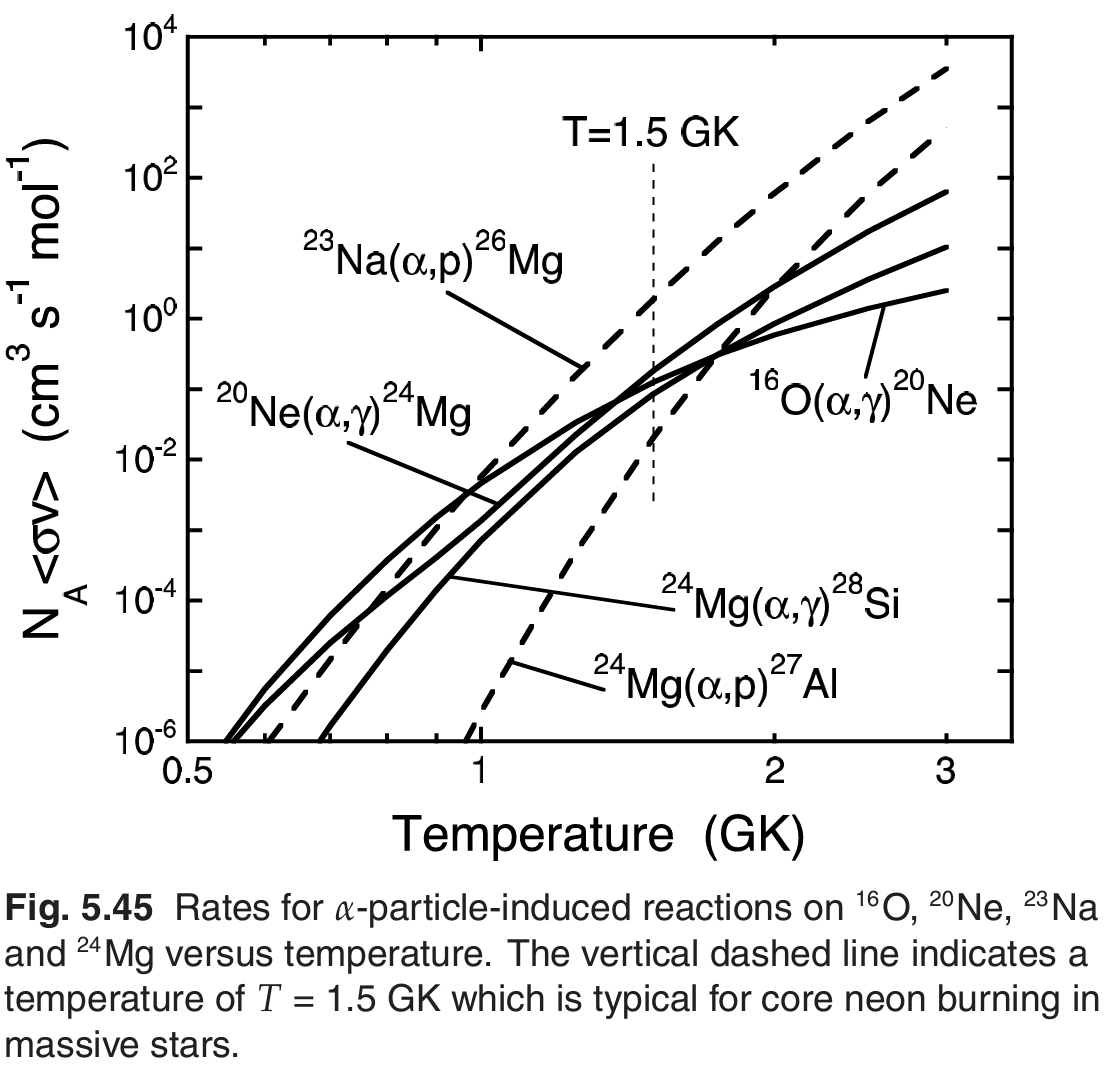
\includegraphics[trim={0cm 0cm 0cm 0cm},clip, keepaspectratio,width=0.9\textwidth]{NeBurning-RR}\label{fig:NeBurning-RR}
\end{figure}
        \end{column}
    \end{columns}
    
            \begin{align*}
                &\int\epsilon_{Ne}(t)\,dt=\frac{N_A\bar{Q}_{Ne}}{2M_{^{20}Ne}}\Delta X_{^{20}Ne}=\num{9.32e22}\Delta X_{^{20}Ne}\si{\mega\ev\per\gram}
            \end{align*}
            Approx factor 3 less energy produced for same amount of consumed fuel comp. to C-Burning
\end{frame}

\begin{frame}{Oxigen Burning ($25\msun{}$, $T\approx\SI{2.2}{\giga\kelvin}$, $\rho\approx\SI{3e6}{\gram\per\cubic\cm}$, $\tau_O\approx\SI{162}{\day}$)}
    \begin{columns}[T]
        \begin{column}{0.45\textwidth}
            Neon exhausted: in stellar core we have $^{16}O$, $^{24}Mg$, $^{28}Si$ - $^{16}O+^{16}O\to ^{32}S$ has lowest coulomb barrier: the compound nucleus is highly excited with mass difference approx \SI{16.5}{\mega\ev}. Primary reactions:
            \begin{align*}
                &^{16}O(^{16}O,p)^{31}P\tag{$Q=\SI{7.7}{\mega\ev}$}\\
                &^{16}O(^{16}O,2p)^{30}Si\tag{$Q=\SI{0.4}{\mega\ev}$}\\
                &^{16}O(^{16}O,\alpha)^{28}Si\tag{$Q=\SI{9.6}{\mega\ev}$}\\
                &^{16}O(^{16}O,2\alpha)^{24}Mg\tag{$Q=\SI{-0.4}{\mega\ev}$}\\
                &^{16}O(^{16}O,d)^{30}P\tag{$Q=\SI{-2.4}{\mega\ev}$}\\
                &^{16}O(^{16}O,n)^{31}S\tag{$Q=\SI{1.5}{\mega\ev}$}
            \end{align*}
        \end{column}
        \begin{column}{0.55\textwidth}
\begin{figure}[!ht]
    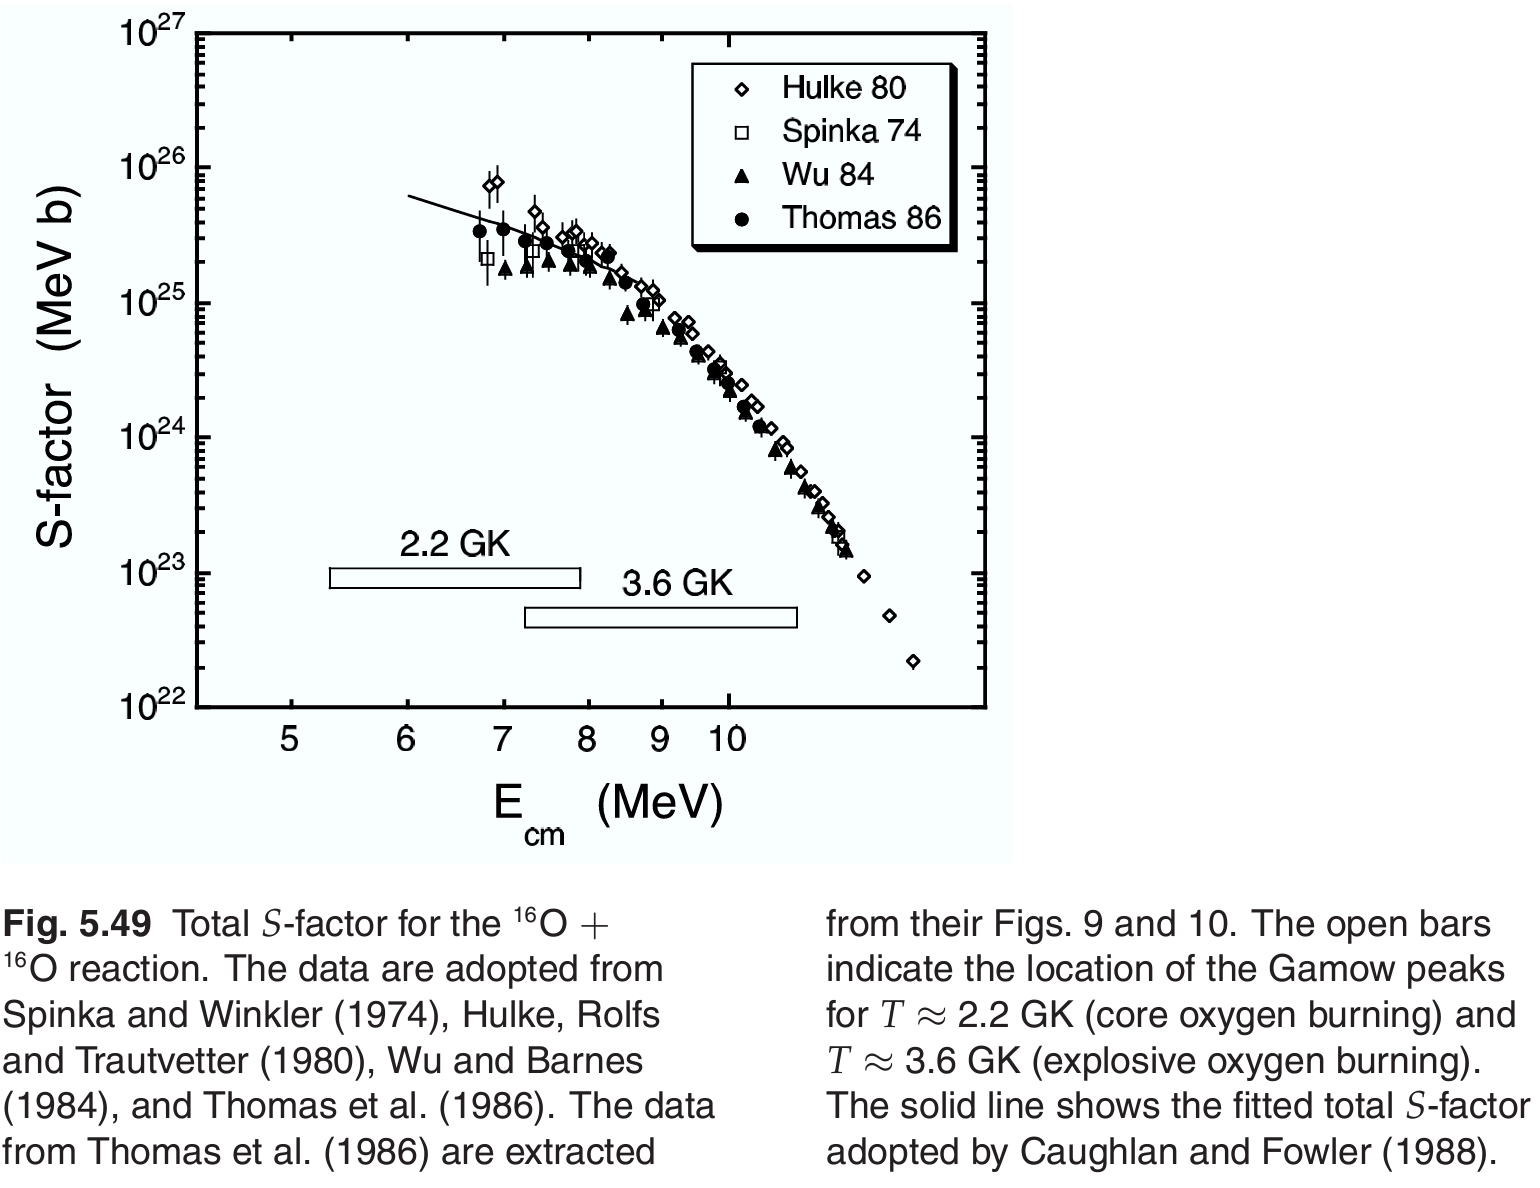
\includegraphics[trim={0cm 0cm 0cm 0cm},clip, keepaspectratio,width=0.5\textwidth]{OBurning-S}\label{fig:OBurning-S}~
    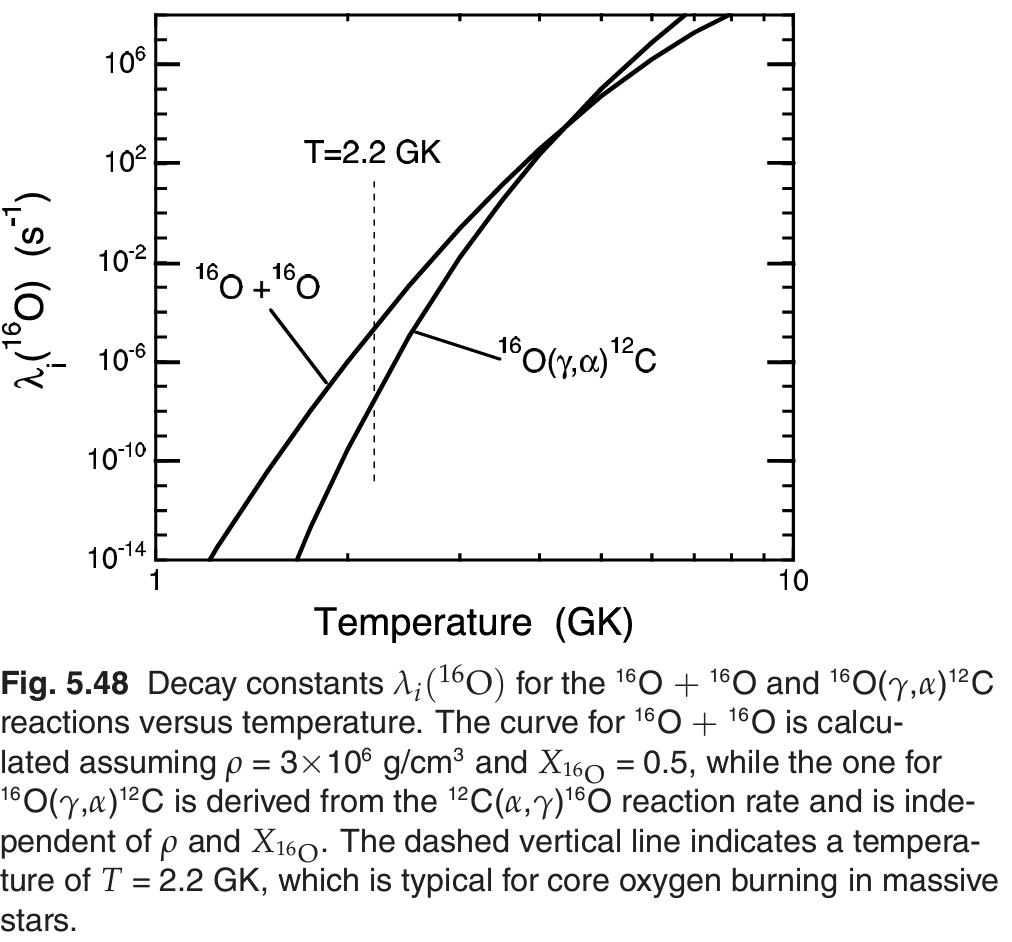
\includegraphics[trim={0cm 0cm 0cm 0cm},clip, keepaspectratio,width=0.5\textwidth]{OBurning-Odepl}\label{fig:OBurning-Odepl}
    
\end{figure}
        \end{column}
    \end{columns}
    Energy sep. for n,p, $\alpha$ are approx. \SI{9}{\mega\ev} except for $^{16}O(\gamma,\alpha)^{12}C$ which is \SI{7.2}{\mega\ev}: $^{16}O$ fusion is major O depletion agent for $T<\SI{4}{\giga\kelvin}$. Proton exit channel dominates at all T: at $T=\SI{2.2}{\giga\kelvin}$ reaction rate contrib. are for p ($62\%$), $\alpha(21\%)$, n($17\%$); secondary reactions contrib. sign. to energy release, $\bar{Q}_O\approx\SI{17.2}{\mega\ev}$ for each $^{16}O+^{16}O$. Electron screening factor $\approx1.3$.
    \begin{align*}
        &\epsilon_O=\frac{\bar{Q}_O}{\rho}r_{^{16}O^{16}O}=\frac{N_A\bar{Q}_O}{512}X_{^{16}O}^2\rho N_A\exv{\sigma v}_{^{16}O^{16}O}=\num{2.03e22}X^2_{^{16}O}\rho N_A\exv{\sigma v}_{^{16}O^{16}O}\si{\mega\ev\per\gram\per\second}\\
        &\epsilon_O(T)=\epsilon_O(T_0)(\frac{T}{T_0})^{34},\ \int\epsilon_O(t)\,dt=\frac{N_A\bar{Q}_O}{2M_{^{16}O}}\Delta X_{^{16}O}=\num{3.24e23}\Delta X_{^{16}O}\si{\mega\ev\per\gram}
    \end{align*}
\end{frame}

\begin{frame}{Nucleosynthesis during O-Burning}
    \begin{columns}[T]
        \begin{column}{0.35\textwidth}
\begin{figure}[!ht]
    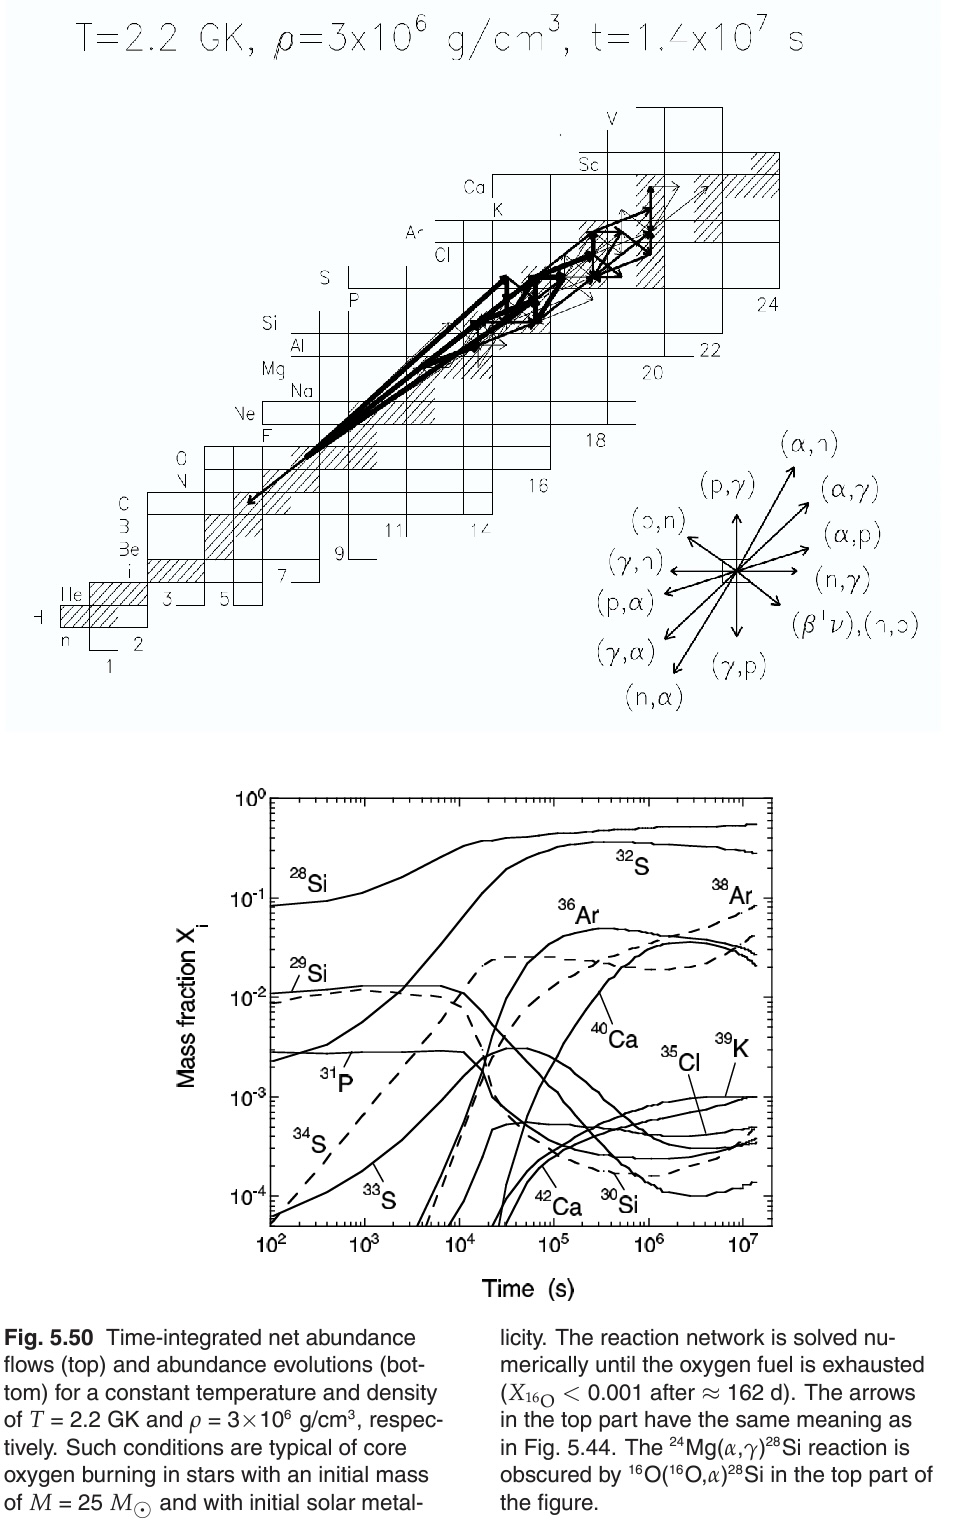
\includegraphics[trim={0cm 0cm 0cm 0cm},clip, keepaspectratio,width=0.95\textwidth]{OBurning-nucl}\label{fig:OBurning-nucl}
\end{figure}
Quasi-equilibrium clusters: several pairs at equil. between forw./reverse photodiss. rate: $A=24-46$, iron peak.
        \end{column}
        \begin{column}{0.65\textwidth}
            At end of Ne burning most abb. species are $^{16}O(X_i=0.77)$, $^{24}Mg(X_i=0.11)$, $^{28}Si(X_i=0.083)$. As O-burn $^{28}Si$, $^{32}S$ increases, also $^{34}S$, $^{35}Cl$, $^{36}Ar$, $^{38}Ar$, $^{39}K$, $^{40}Ca$, $^{42}Ca$ also increase.
            \begin{itemize}
                \item Production of $^{28}Si$, $^{32}S$
                    \begin{align*}
                        &^{16}O(^{16}O,p)^{31}P(p,\gamma)^{32}S\\
                        &^{16}O(^{16}O,p)^{31}P(p,\alpha)^{28}Si\\
                        &^{16}O(^{16}O,\alpha)^{28}Si\\
                        &^{16}O(^{16}O,n)^{31}S(\gamma,p)^{30}P(\gamma,p)^{29}Si(\alpha,n)^{32}S
                    \end{align*}
                \item $^{31}S$, $^{30}P$ have rel. low sep energy ($S_p\approx\SI{6.1}{\mega\ev},\SI{5.6}{\mega\ev}$): photodisintegration domin. over $^{31}S(\beta^+\nu)^{31}P$ still relevant.
                \item Sulfur-32: $^{28}S(\alpha,\gamma)^{32}S$ and converted back via $^{32}S(n,\gamma)^{33}S(n,\alpha)^{30}Si(p,\gamma)^{31}P$ or converted to heavier $^{32}S(\alpha,p)^{35}Cl(p,\gamma)^{36}Ar$ and so on.
                \item Depletion of $^{24}Mg$ via liberated $\alpha$: $^{24}Mg(\alpha,\gamma)^{28}Si$ and $^{24}Mg(\alpha,p)^{27}Al$.
                \item Neutron excess increases by factor 5: $^{31}S(\APelectron\nu)^{31}P$, $^{30}P(\APelectron\nu)^{30}Si$, and \Pelectron-capture $^{33}S(\Pelectron,\nu)^{33}P$, $^{35}Cl(\Pelectron,\nu)^{35}S$, $^{37}Ar(\Pelectron,\nu)^{37}Cl$.
                \item Explosive O-burning is bel. major source of $^{28}Si$, $^{32,33,34}S$, $^{35}Cl$, $^{36,38}Ar$, $^{39,41}K$, $^{40,42}Ca$
                \item Reduced lifetime against $\beta$-decay
                \item At end of O-burning T is suff. high to produce light particles via photodiss.
            \end{itemize}
        \end{column}
    \end{columns}
\end{frame}

\begin{frame}{Si-Burning ($25\msun{}$, $T\approx\SI{3.6}{\giga\kelvin}$, $\rho\approx\SI{3e7}{\gram\per\cubic\cm}$, $\tau_{Si}\approx\SI{4000}{\second}$)}
    \begin{columns}[T]
        \begin{column}{0.35\textwidth}
\begin{figure}[!ht]
    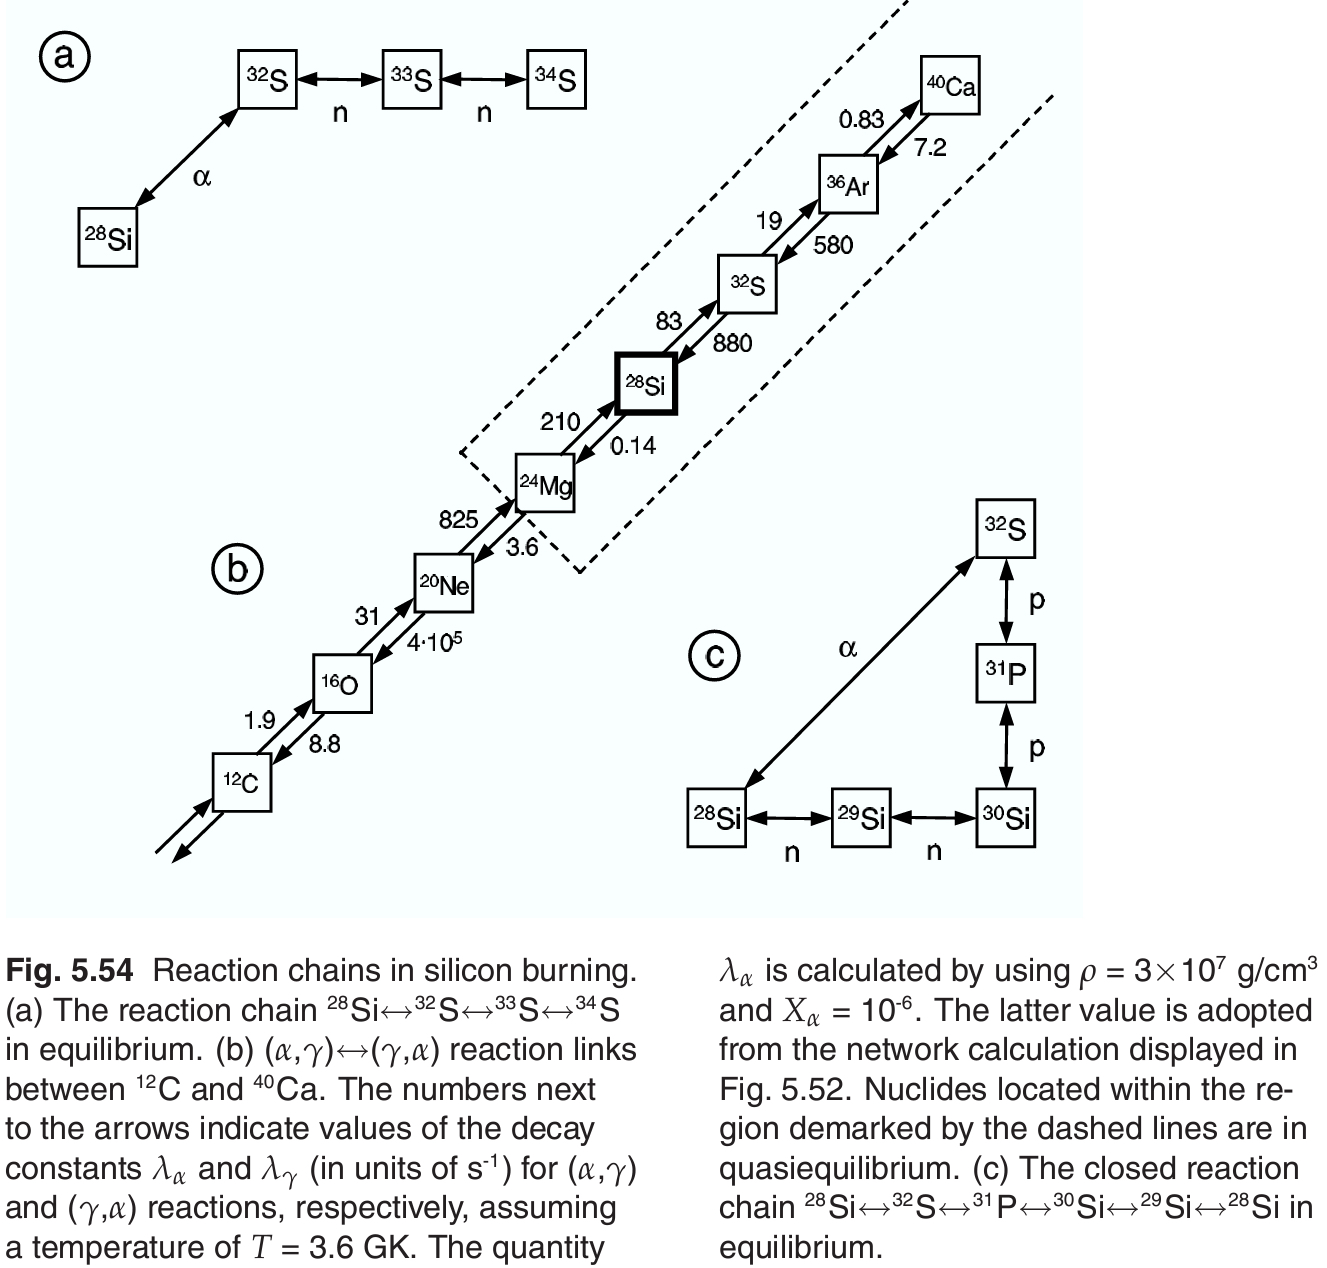
\includegraphics[trim={0cm 0cm 0cm 0cm},clip, keepaspectratio,width=0.95\textwidth]{SiBurning-chains}\label{fig:SiBurning-chains}
    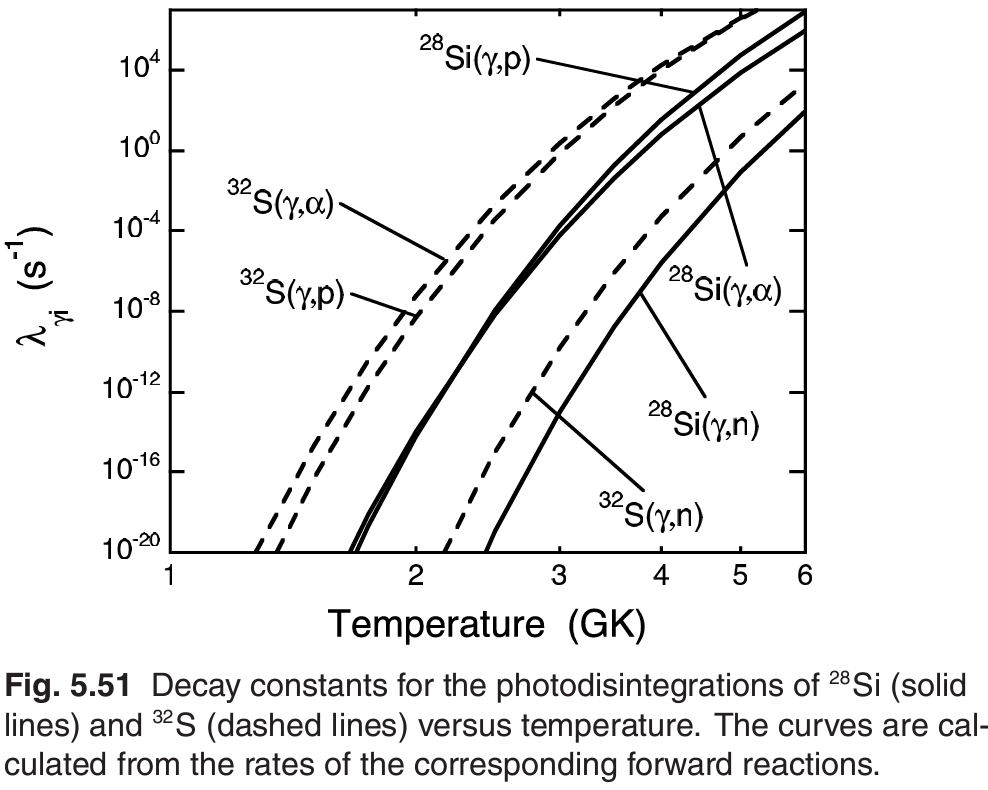
\includegraphics[trim={0cm 0cm 0cm 0cm},clip, keepaspectratio,width=0.95\textwidth]{SiBurning-lambda}\label{fig:SiBurning-lambda}
\end{figure}
            
        \end{column}
        \begin{column}{0.65\textwidth}
            Photodis. rearrangement similar to Ne-burning but on larger scale: $^{28}Si+^{28}Si$ and $^{28}Si+^{32}S$ have high Coulomb barrier, so reactions go via photodis. of less bound nuclei and captures of light part.
            \begin{align*}
                &S_p(^{32}S)\approx\SI{8.9}{\mega\ev}, S_n(^{32}S)\approx\SI{15}{\mega\ev}, S_{\alpha}(^{32}S)\approx\SI{10}{\mega\ev}\\
                &S_p(^{28}Si)\approx\SI{11.6}{\mega\ev}, S_n(^{28}Si)\approx\SI{17.2}{\mega\ev}, S_{\alpha}(^{28}Si)\approx\SI{10}{\mega\ev}
            \end{align*}
            Above $T=\SI{2}{\giga\kelvin}$ $^{32}S$ will be consumed via: $^{32}S(\gamma,\alpha)^{28}P$, $^{32}S(\gamma,p)^{31}P(\gamma,p)^{30}Si(\gamma,n)^{29}Si(\gamma,n)^{28}Si$; T increases further to becomes disintegration of $^{28}Si$ ($^{28}Si(\gamma,p)^{27}Al$, $^{28}Si(\gamma,\alpha)^{24}Mg$: energy sep. for latter is much smaller, Coulomb barrier for ejected particles, reduced particle width of res).
            \begin{align*}
                &\epsilon_{Si}=\frac{Q_{2^{28}Si\to^{56}Ni}}{\rho}r_{2^{28}Si\to^{56}Ni}\approx \frac{Q_{2^{28}Si\to^{56}Ni}}{\rho}r_{^{24}Mg(\gamma,\alpha)^{20}Ne}\\
                &=\frac{Q_{2^{28}\to^{56}Ni}}{\rho}N_{^{24}Mg}\lambda_{\gamma\alpha}(^{24}Mg)\\
                &\epsilon_{Si}\approx\num{1.2985e34}X_{^{28}Si}(\frac{2X_{^{28}Si}}{1-X_{^{28}Si}})^{\frac{1}{7}}\exp{-\frac{142.12}{T_9}}T_9^{\frac{3}{2}}N_A\exv{\sigma v}_{^{20}Ne}\si{\mega\ev\per\gram\per\second}\\
                &\epsilon_{Si}(T)=\epsilon_{Si}(T_0)(\frac{T}{T_0})^{47}\tag{$T_0=\SI{3.6}{\giga\ev}$}\\
                &\bar{Q}_{Si}\approx Q_{2^{28}Si\to ^{56}Fe}=\SI{17.62}{\mega\ev}\\
                &\int\epsilon_{Si}(t)\,dt=\frac{N_A\bar{Q}_{Si}}{2M{^{28}Si}}\Delta X_{^{28}}=\num{1.9e23}\Delta X_{^{28}Si}
            \end{align*}
        \end{column}
    \end{columns}
\end{frame}

\begin{frame}{Si-Burning: Abundance flows}
    \begin{columns}[T]
        \begin{column}{0.4\textwidth}
\begin{figure}[!ht]
    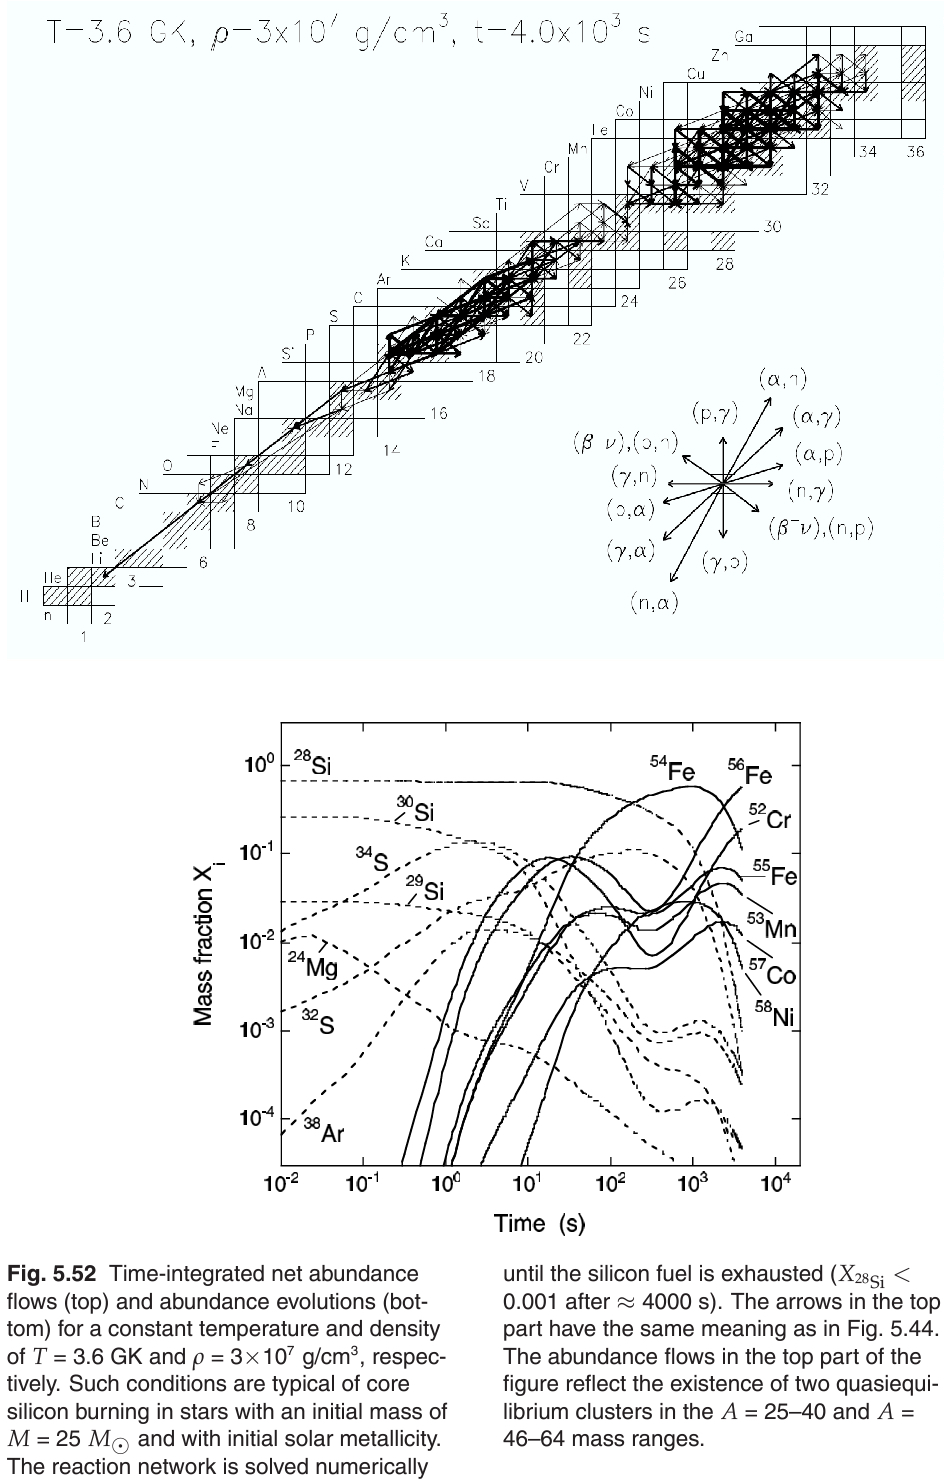
\includegraphics[trim={0cm 0cm 0cm 0cm},clip, keepaspectratio,width=0.95\textwidth]{SiBurning-abbflows }\label{fig:SiBurning-abbflows }
\end{figure}
        \end{column}
        \begin{column}{0.6\textwidth}
            \begin{itemize}
                \item Thermally excited levels have big effect on decay const. for weak interactions and rates of many for./rever. reactions.
                \item Quasiequilibrium clusters: $A=25-40$, $A=46-64$
                \item At end of Si-burning stellar matter is $^{56}Fe$ ($X_f=0.56$), $^{52}Cr(X_f=0.19)$, $^{54}Fe(X_f=0.11)$, $^{55}Fe(X_f=0.05)$, $^{53}Mn(X_f=0.034)$
                \item Neutron excess remains almost constant until iron peak is reached then increases sign.: $^{53}Mn(\Pelectron,\nu)^{53}Cr$, $^{54}Fe(\Pelectron,\nu)^{54}Mn$, $^{55}Fe(\Pelectron,\nu)^{55}Mn$, $^{55}Co(\Pelectron,\nu)^{55}Fe$. At end $\eta_f\approx0.067$
            \end{itemize}
        \end{column}
    \end{columns}
\end{frame}

\begin{frame}{Nuclear Statistical equilibrium and $\alpha$ freeze-out}
    \begin{columns}[T]
        \begin{column}{0.4\textwidth}
            
        \end{column}
        \begin{column}{0.6\textwidth}
            \begin{itemize}
                \item Every nuclide in the network is in equilibrium: NSE.
                \item While shock wave after massive stars explode move outward stellar matter in NSE cools and expands: denote $T_{\alpha}$ temperature at which $\alpha$ particles are not at equilibrium.
                \item If $T_{\alpha}$ high such that few $\alpha$ presents:  When T falls below $T_{\alpha}$ photodisintegration fails to produce enough $\alpha$ particles. Particles-poor freeze-out.
                \item If $T_{\alpha}$ low such that abb. of $\alpha$ is large: as T falls toward $T_{\alpha}$ free $\alpha$ tends to merge into iron peak $3\alpha\to^{12}C(\alpha,\gamma)^{16}O\ldots^{52}Fe(\alpha,\gamma)^{56}Ni$; when $T<T_{\alpha}$ suff. rapidly $\alpha$ can't be converted rapidly enough: excess of $\alpha$ particles. $\alpha$-rich freeze-out.
            \end{itemize}
        \end{column}
    \end{columns}
    
\end{frame}
